% AUTO-GENERATED CONFLICT REVIEW FILE
% latexdiff was not available for this file.

===== LOCAL VERSION =====
\documentclass[11pt]{article}

\usepackage{amsmath,amssymb,amsfonts}
\usepackage{xcolor}
\usepackage{authblk}
\usepackage{geometry}
\usepackage{graphicx}
\usepackage{hyperref}
\usepackage{chngcntr}
\geometry{margin=1in}
\graphicspath{{figures/}}
\DeclareGraphicsExtensions{.pdf,.png,.jpg}
\renewcommand{\vec}[1]{\boldsymbol{#1}}
\newcommand{\blue}[1]{{\color{blue}#1}}
\newcommand{\purple}[1]{\textcolor{purple}{#1}} 
\newcommand{\red}[1]{{\color{red}#1}}
\renewcommand\Authfont{\normalsize}
\renewcommand\Affilfont{\small}
\counterwithout{table}{section}
\renewcommand{\thetable}{\arabic{table}}

\title{Hippopede Universe as a toy model of late-linear expansion}
\author[1,2]{Robert Monjo}
\author[3]{Manel Romero}
\author[4]{Ardra E. Sasi}
\affil[1]{Department of Mathematics, CUNEF University, Calle Almansa 101, Madrid 28040, Spain}
\affil[2]{Centro de Estudios Cosmologicos ``Prof. Jaime Roessler Bonzi'', Facultad de Ciencias, Universidad de Chile, Las Palmeras 3425, \~Nunoa, Santiago 7750000, Chile}
\affil[3]{Area of Chemistry, University of Barcelona, Campus Diagonal: Av. Joan XXIII, 27-31, 08028 Barcelona, Spain}
\affil[4]{School of Pure and Applied Physics
Mahatma Gandhi University, Priyadarsini Hills P.O. Athirampuzha, Kottayam, Kerala 686560, India}
\date{}

\begin{document}

\maketitle

\begin{abstract}

The hippopede is a classical quartic curve with a long history in geometry, yet it also offers a suggestive reinterpretation in modern embedding approaches. In this work we show that its defining relation can be recast as a null quadratic constraint in an auxiliary pseudo-Euclidean space, thereby placing the extended hippopede hypersurface in direct analogy with the ambient-space constructions commonly used for de Sitter and anti de Sitter geometries. We then apply the same quartic structure to a four-dimensional toy universe whose large-$t$ limit consists of two tangent $3$-spheres, so that the model becomes a simple laboratory for asking whether a hyperconical late-time coasting law can emerge together with a distinct early-time acceleration.

\end{abstract}

\section{Introduction}

\subsection{Motivation}

Model-dependent probes such as BAO and CMB fits, and more direct determinations based on cosmic chronometers (CC) and Type Ia supernovae (SNe Ia), do not always favour the same late-time expansion history. This discrepancy is visible both in the local Hubble tension and in the broader discussion of how background expansion should be inferred from intrinsic versus projection-dependent observables. In hyperconical approaches this distinction is especially relevant, because an apparently accelerated phenomenology can arise from the projection map even when the underlying ambient-space expansion remains asymptotically linear \cite{monjo2018projected, monjo2023hubble}.

A natural starting point for the present work is the long-standing interest in coasting cosmologies, namely models for which the late-time scale factor behaves approximately as $a(t)\propto t$. Such scenarios were studied early on by John et al. \cite{john2000coasting, John2019} as viable alternatives to standard decelerating or accelerated backgrounds, and more recently they have reappeared in hyperconical modified-gravity constructions where the linear law is tied to an ambient-space geometric constraint \cite{monjo2017hyperconical, Monjo_2024, Monjo_2025}. Within that framework, recent astrophysical tests indicate that the model can remain phenomenologically competitive beyond galactic rotation curves: hydrostatic-equilibrium analyses of X-COP clusters show good agreement in hot-gas-dominated regions beyond $\sim1\,\mathrm{Mpc}$, while galaxy--galaxy weak-lensing reconstructions yield flat circular velocities on megaparsec scales that compare favorably with MOND in the same regime \cite{monjo2025clusters, monjo2025lensing}.

The main cosmological motivation for relaxing exact coasting at all epochs comes from primordial nucleosynthesis. In a strictly linear expansion, $H(t)=1/t$, the Universe remains older at a fixed temperature than in the standard radiation-dominated scenario, so weak interactions stay effective for longer and the neutron-to-proton ratio freezes out under different conditions. This alters the synthesis window for light nuclei: in particular, it tends to overproduce helium and strongly affects deuterium survival unless additional assumptions are introduced \cite{sethi1999coasting, dev2002coasting}. For that reason, even if a late coasting regime is phenomenologically attractive, one is naturally led to explore toy geometries in which the large-$t$ behaviour remains asymptotically linear while the early-time acceleration differs from zero. The hippopede universe proposed below is meant precisely in that spirit: it is not offered as a realistic cosmology, but as a controllable biaxial toy model interpolating between a regular quartic geometry and a hyperconical-like late regime.

\subsection{Hippopede curve}
Algebraic curves of low degree have long played a role not only in classical geometry but also in astronomical modelling and, more recently, in modern theoretical physics. Among these curves, the \emph{hippopede} occupies a historically interesting position. The curve was already known in Greek geometry and is traditionally associated with the work of Eudoxus and later commentators such as Proclus, appearing in discussions of planetary motion and spherical constructions \cite{Gregory_2011, Taub2020, BotteriCasazza2023}. In modern mathematical terminology, the hippopede is a quartic plane curve that can be written in implicit form as the set of points $(x,y) \in \mathbb{R}^2$ satisfying:
\begin{equation}
    k x^2 + y^2 - (x^2+y^2)^2 = 0
\end{equation}
where $(x,y)$ are the Cartesian coordinates and $k > 0$ is a positive real constant.


The geometry of this curve and related quartic curves has been discussed in classical works on plane algebraic curves and in modern mathematical treatments of special curves. Standard references include the classical monograph of Lawrence \cite{lawrence1972catalogue} and more recent surveys of plane quartics such as those by Gibson \cite{gibson2001elementary}. From the viewpoint of differential geometry, the curve can also be viewed as a deformation of the circle controlled by the parameter $k$. Writing $k=4t^2$ and introducing polar coordinates $(r,\theta)$ defined by $x=r\cos\theta$ and $y=r\sin\theta$, the defining equation becomes $r^2 = 4t^2\cos^2\theta + \sin^2\theta$. This representation shows that the curve can be regarded as a deformation of the circle in which the radial coordinate depends on the polar angle. When $t=\tfrac12$ (equivalently $k=1$) the curve reduces to the unit circle. For $t >\tfrac12$ the curve develops the characteristic shape of the hippopede, elongated along the horizontal axis.

From the algebraic viewpoint the curve is a quartic plane curve symmetric under reflections across both coordinate axes. Its intersection with the coordinate axes is easily determined: the curve passes through $(0,\pm1)$ independently of the value of $k$, while its intersection with the horizontal axis occurs at $(\pm 2t,0)$. These properties make the hippopede a particularly simple example of a quartic curve whose geometry is controlled by a single parameter.

\subsection{Hyperconical, \textit{de Sitter} and \textit{anti de Sitter} geometries}

The hyperconical universe $\mathcal{H}^4$ is mathematically defined as the null hypersurface embedded in a pseudo-Euclidean manifold (flat ambient space) of signature $s=(1,4)$ or $s=(4,1)$, which is usually referred to as 5-dimensional Minkowskian spacetime $\mathbb{R}^s$ \cite{monjo2017hyperconical, Monjo_2024}. For instance, the $(4,1)$ convention can be written as follows:
\begin{equation}
\mathcal{H}^4:=\left\{q=(t,\vec{\rho})\in\mathbb{R}^{4,1}\;:\;-t^2+\|\vec{\rho}\|_{\scriptscriptstyle{(4,0)}}^2=0\right\},
\end{equation}where $\|\vec{\rho}\|_{\scriptscriptstyle{(4,0)}} ^2$ represents the quadratic form of $\vec{\rho} = (x,y,z,u)$ in $\mathbb{R}^4$, that is, $\|\vec{\rho}\|_{\scriptscriptstyle{(4,0)}} ^2 = x^2+y^2+z^2+u^2$. Equivalently, on each constant-$t$ slice one has $\|\vec{\rho}\|_{\scriptscriptstyle{(4,0)}} =t$, so the spatial section is a 3-sphere of radius $t$ and the resulting background expands linearly. By contrast, the 4-dimensional de Sitter (dS${}_4$) spacetime is described by the hyperboloid $-X_0^2+X_1^2+X_2^2+X_3^2+X_4^2=\alpha^2$ in the same ambient-space $\mathbb{R}^{4,1} \ni (X_0, \dots X_4) = X$, but with nonzero curvature radius $\alpha = \|X\|_{\scriptscriptstyle{(4,1)}}$. Within this embedding picture, the hyperconical universe may be regarded as the degenerate limit $\alpha\to0$ of the dS${}_4$ family, for which the regular hyperboloid collapses to the null cone. It is therefore better described as a singular limit of dS geometry than as an ordinary dS spacetime. 

Finally, a $4$-dimensional \textit{anti de Sitter} (AdS${}_4$) spacetime is a pseudo-Riemannian manifold embedded by increasing up to two time coordinates $(t_1, t_2)$, which satisfy $-t_1^2-t_2^2+X_1^2+X_2^2+X_3^2 = - \alpha$ in a pseudo-Euclidean space $\mathbb{R}^{3,2}$ with signature $(3,2)$.  Thse constructions provide a powerful geometric representation of constant curvature cosmological spacetimes and is standard in the literature on relativistic cosmology and quantum field theory in curved spacetime \cite{hawking1973large, spradlin2001les}.

What these constructions share is the quadratic embedding language, and this is exactly the bridge on which the present toy model is built. The hippopede extension sits between both pictures: like the hyperconical case, it has an asymptotically linear radius; like the dS/AdS constructions, it is most naturally understood through a higher-dimensional quadratic relation. Hyperconical models have been proposed precisely because they realize a linear late expansion law in a natural embedding setting \cite{monjo2017hyperconical}. It is therefore natural to ask whether nearby toy models can preserve the asymptotic coasting behaviour $a(t)\propto t$ while allowing a different acceleration pattern during early epochs. The higher--dimensional hippopede provides a minimal laboratory for that question: it keeps the same large-$t$ linear scaling along the expanding directions, but it regularizes the exact hyperconical behaviour by a finite angular term that modifies the early dynamics.


The logic of the paper is therefore fourfold: first, we identify the correct high--dimensional extension of the quartic relation; second, we extract its large-$t$ limit as two tangent hyperspheres, with the intention of a hyperconical toy universe; third, we compute the corresponding directional Hubble and acceleration functions; and fourth, we relate the resulting quartic toy model to the ambient-space construction used for dS/AdS geometries.


\section{Data and Methods}

\subsection{Data}

We used observed estimates of the deceleration parameter collected from: i) the present deceleration estimates $q_0=-0.364\pm0.032$ together with the transition redshift estimate $z_t=0.597\pm0.214$ from the combined CC+Pantheon+SH0ES+BAO analysis \cite{myrzakulov2025q0}; ii) the cosmographic estimate $q_0=-0.50\pm0.20$ obtained from fast radio bursts (FRB) combined with supernovae (SNe) in \cite{gao2024frb}; iii) the screened meta-analytic transition estimate $z_t=0.64\pm0.16$ from the latest $H(z)$ compilation analysis of \cite{hu2025transition}. Moreover, observed estimates of normalized Hubble factor $E_{\mathrm{obs}}(z)=H(z)/H_0$ were computed from the CC measurements, with $H_0=70~\mathrm{km\,s^{-1}\,Mpc^{-1}}$ (Table \ref{tab:cc_data_figures}).

For the dedicated low-to-intermediate redshift constraints on the projected model, we additionally use two complementary datasets. The DES-SN5YR Type Ia supernova sample \cite{abbott2024dark} contains 1829 supernovae over the interval $0.025 \le z \le 1.3$. The compressed DESI DR1 baryon acoustic oscillation catalogue \cite{adame2025desi} provides measurements of $D_M/r_s$, $D_H/r_s$, and $D_V/r_s$ in six galaxy and quasar tracer bins centered at $z_{\rm eff}=0.295$, $0.510$, $0.706$, $0.930$, $1.317$, and $1.491$. In this first geometric analysis we exclude the Ly$\alpha$ forest point near $z_{\rm eff}\simeq2.33$, so that the fit remains restricted to the lower-redshift window most directly comparable with the supernova sector.

\begin{table}[h]
\centering
\small
\caption{Observational inputs used in this work.}
\label{tab:dataset_summary}
\begin{tabular}{lll}
\hline
Redshift range & Observable(s) & Dataset \\
\hline
local to intermediate & $q_0$, $z_t$ & Cosmographic constraint \cite{myrzakulov2025q0,gao2024frb,hu2025transition} \\
low to intermediate & reconstructed $q(z)$ and $E(z)$ & CC+Pantheon$+$ GaPP \cite{seikel2012gapp} \\
$0.025$--$1.3$ & SN distance moduli & *DES-SN5YR \cite{abbott2024dark} \\
$0.295$--$1.491$ & $D_M/r_s$, $D_H/r_s$, $D_V/r_s$ & *DESI DR1 BAO \cite{adame2025desi} \\
\hline
\end{tabular}
\end{table}


\begin{table}[h]
\label{tab:cc_data_figures}
\centering
\small

\caption{Observed values of the Hubble parameter according to the cosmic chronometers considered.}

\begin{tabular}{lll}
\hline
$z$ & $H(z)$ [km s$^{-1}$ Mpc$^{-1}$] &  Cosmic chronometers \\
\hline
0.07, 0.12, 0.20, 0.28 & 69.0$\pm$19.6,\;68.6$\pm$26.2,\;72.9$\pm$29.6,\;88.8$\pm$36.6 & Zhang et al. \cite{zhang2014hubble} \\
0.40, 0.48 & 95.0$\pm$17.0,\;97.0$\pm$62.0 & Stern et al. \cite{stern2010chronometers} \\
0.75 & 105.0$\pm$7.9(stat)$\pm$7.3(sys) & Jimenez et al. \cite{jimenez2023photometry} \\
0.80 & 113.1$\pm$15.1(stat)$^{+29.1}_{-11.3}$(sys) & Jiao et al. \cite{jiao2023legac} \\
1.26 & 135.0$\pm$35.0 & Tomasetti et al. \cite{tomasetti2023vandels} \\
\hline
\end{tabular}

Note:  *Likelihood constraint on $\alpha_{\mathrm{eff}}$
%$0.07$--$1.26$ & $H(z)$, hence $E(z)=H/H_0$ & Cosmic chronometers \\


\end{table}

Finally, Gaussian-process reconstructions obtained with the original GaPP logic are included in order to compare the centered hippopede histories with model-independent reconstructions of both $q(z)$ and $E(z)$ based on CC+Pantheon$+$ data \cite{seikel2012gapp}.



\subsection{Model}

\subsubsection{The coasting hippopede universe}

Let $(t, \vec \rho) = (t,x,y,z,u)\in\mathbb{R}^{1,4}$, and consider the hypersurface
\begin{equation}
\label{eq:hippopede_univ}
 x^2 + y^2 + z^2 + 4t^2 u^2 = (x^2 + y^2 + z^2 + u^2)^2 .
\end{equation}
defined as an upper-dimensional extension of the hippopede curve.

 Let $\rho^2 := \|\vec \rho\|_{\scriptscriptstyle{(4,0)}}^2$ with $\|\vec \rho\|_{\scriptscriptstyle{(4,0)}}^2=x^2 + y^2+z^2 + u^2 =: r^2 + u^2$ and introduce spherical coordinates around the distinguished $u$-axis,
\begin{equation}\label{eq:angle-constraint}
u=\rho\cos\chi,\qquad r=\rho\sin\chi.
\end{equation}
Then Eq.~\eqref{eq:hippopede_univ} becomes
\begin{equation}
\label{eq:hippopede_univ2}
\rho^2=\sin^2\chi+4t^2\cos^2\chi.
\end{equation}
Introducing the auxiliary coordinates
$t_1:=2t\cos\chi,\; t_2:=\sin\chi$,
the same relation is exactly equivalent to the null condition $\vec{\rho}^2-t_1^2-t_2^2=0$,
in a 6D ambient space with pseudo-Euclidean metric of signature $(2,4)$ or $(4,2)$. According to Eq. \ref{eq:angle-constraint}, the 4D hippopede hypersurface is therefore given by the dipolar-angle constraint $u^2-{\vec \rho}^2(1-t_2^2) = 0$ of the 6D null hypercone in the ambient space, where $u$ is the fourth coordinate of $\vec \rho$. This is the minimal consistent immersion formulation of the toy model, which is equivalent to encode the quartic hypersurface through a nonlinear map from the physical variables $(t,\chi)$ into an auxiliary null cone (Eq. \ref{eq:hippopede_univ2}). This exact expression already displays two key points: i) it contrasts with the \textit{light cone} $\{p = (t,\vec{\rho}) \in \mathbb{R}^{1,4}\;:\; \|p\|^2 = 0\}$ defined in the $(1,4)$-signature hyperconical universe; ii) along every direction with $\cos\chi\neq0$, the size of the configuration grows linearly with $t$ for large times, as in the $\mathbb{R}^{1,4}$ case. More precisely,
\begin{equation}
\rho(t,\chi)=2|{\cos\chi}|\,t+\frac{\sin^2\chi}{4|{\cos\chi}|\,t}+O(t^{-3})\qquad (t\to\infty).
\end{equation}
The leading term
\begin{equation}
\rho_{\infty}(t,\chi)=2|{\cos\chi}|\,t
\end{equation}
is exactly the dipolar equation of the union of the two tangent $3$-spheres
\begin{equation}
x^2+y^2+z^2+(u-t)^2=t^2,\qquad x^2+y^2+z^2+(u+t)^2=t^2.
\end{equation}
Indeed, each sphere of radius $t$ centered at $u=\pm t$ satisfies $\rho=2t|\cos\chi|$. In this sense the quartic hypersurface interpolates between a smooth finite-$t$ geometry and a double-sphere large-$t$ limit, which is the natural place to import the hyperconical-universe intuition into the hippopede setting.

At the purely geometric level, the most immediate ``origin-based'' reading of the quartic hypersurface is simply $a_{\chi}(t):=\rho(t,\chi)$.  If one now reads $t$ as a cosmic parameter and keeps the angular sector $\chi$ fixed, the directional scale factor of this toy model is
\begin{equation}
a_\chi(t):=\rho(t,\chi)=\sqrt{\sin^2\chi+4t^2\cos^2\chi}.
\end{equation}
Its directional Hubble $H_\chi(t)= \dot a_\chi / a_\chi$ and acceleration $\ddot a_\chi(t)$ determine its deceleration function as $q_\chi(t):= - a_\chi\ddot a_\chi / \dot a_\chi^2 = - a_\chi a_\chi\ddot / H_\chi(t)^2$. We remark on that prescription because it yields closed analytic expressions and provides a useful first contrast with the hyperconical case with pure linear expansion (see Appendix). However, the numerical results eventually adopted for the two definitive comparison figures are based instead on a centered effective scale factor measured with respect to the center of curvature of one asymptotic tangent branch.

\begin{figure}[t]
\centering

\includegraphics[width=0.78\textwidth]{hippopede_growth_3d}
\caption{Three-dimensional visualization of the nested hippopede hypersurfaces associated with increasing values (0.5, 1, 2 and 3.0) of the parameter $t$. The distinguished axis is $u$, while the orthogonal directions are represented through $(\sqrt{x^2+y^2},z)$. As $t$ grows, the quartic hypersurface approaches the large-time limit formed by two tangent 3-spheres centered at $u=\pm t$, making explicit the emergence of an asymptotically hyperconical coasting regime.}
\label{fig:hippopede_growth_3d}
\end{figure}


\subsection{\blue{Centered prescription}}

\blue{The analytic scale factor $a_\chi(t)=\rho(t,\chi)$ introduced above is the most direct reading of the quartic hypersurface, but the large-$t$ tangent-sphere limit also suggests a second effective radius measured from the center of curvature of one asymptotic branch. In the numerical figures we therefore define, on the $+u$ branch, the centered effective scale factor}
\begin{equation}
\blue{
a_{c,\chi}(t):=\sqrt{r^2+(u-t)^2}
=\sqrt{\rho(t,\chi)^2+t^2-2t\,\rho(t,\chi)\cos\chi}.
}
\end{equation}
\blue{This prescription is not meant to replace the intrinsic quartic relation; it is introduced only as a figure-level effective radius motivated by the double-sphere asymptotic geometry. The corresponding centered redshift, Hubble and deceleration functions used in the simulations are}
\begin{equation}
\blue{
1+z_\chi(t)=\frac{a_{c,\chi}(t_0)}{a_{c,\chi}(t)},\qquad
H_{c,\chi}(t)=\frac{\dot a_{c,\chi}(t)}{a_{c,\chi}(t)},\qquad
E_\chi(z)=\frac{H_{c,\chi}(t)}{H_{c,\chi}(t_0)},
}
\end{equation}
\begin{equation}
\blue{
q_\chi(z)=-\frac{a_{c,\chi}(t)\,\ddot a_{c,\chi}(t)}{\dot a_{c,\chi}(t)^2},
}
\end{equation}
\blue{with the derivatives evaluated numerically along each centered history. In the final comparison figures we fix $t_0=3$ and show the angular sectors $\chi=0^\circ,15^\circ,30^\circ,45^\circ,60^\circ,85^\circ$. The case $\chi=0^\circ$ is then identical to the unprojected hyperconical/coasting reference of the same centered prescription.}

\subsection{\blue{Projected prescription}}

\blue{To generate the projected simulations, we keep the same centered histories but remap them through the projected-hyperconical construction used by Monjo in the inhomogeneous hyperconical programme \cite{monjo2017hyperconical, monjo2018projected, monjo2020lagrangian, monjo2023hubble, Monjo_2024}. In the notation of \cite{monjo2018projected}, let}
\begin{equation}
\blue{
\xi_1(x):=\int_{0}^{x}\frac{\sqrt{1-(1-b)^2}}{b\left[2(b-1)+1\right]}\,d\tilde x,
\qquad
b=b(\tilde x):=\sqrt{1-\tilde x^2},
}
\end{equation}
\blue{be the dimensionless line-of-sight function of the $k=1$ hyperconical model, and define}
\begin{equation}
\blue{
x(z):=\xi_1^{-1}(\ln(1+z)).
}
\end{equation}
\blue{The preferred $\gamma$-projection is then written as}
\begin{equation}
\label{eq:projection_map}
\blue{
f_{\hat r}^{\alpha}(x):=
2\arctan\!\left[
\frac{\gamma(x)/2}{\left(1-\gamma(x)/\gamma_U\right)^\alpha}
\right],
}
\end{equation}
\blue{where}
\begin{equation}
\blue{
\gamma(x):=\arctan\!\left(\frac{x}{\sqrt{1-x^2}}\right)
,
\qquad \gamma_U:=\gamma(x_{\max}).
}
\end{equation}
\blue{For the $k=1$ hyperconical domain one has $x_{\max}=\sqrt{3}/2$, hence}
\begin{equation}
\blue{
\gamma_U=\arctan\!\left(\frac{\sqrt{3}/2}{1/2}\right)=\arctan(\sqrt{3})=\frac{\pi}{3}.
}
\end{equation}
\blue{The projected hyperconical proper distance is therefore}
\begin{equation}
\blue{
\hat r(z)= f_{\hat r}^{\alpha}\!\left(x(z)\right)
= f_{\hat r}^{\alpha}\!\left(\xi_1^{-1}(\ln(1+z))\right),
}
\end{equation}
\blue{and the associated projected reference Hubble function is defined by}
\begin{equation}
\blue{
\hat H(z):=\left(\frac{d\hat r}{dz}\right)^{-1},
\qquad
E_{\mathrm{hyp}}^{\mathrm{proj}}(z)=\frac{\hat H(z)}{\hat H(0)}.
}
\end{equation}
\blue{Each centered hippopede simulation is then projected through the common redshift remapping}
\begin{equation}
\blue{
z^*=E_{\mathrm{hyp}}^{\mathrm{proj}}(z)-1,
\qquad
E^{\mathrm{proj}}_\chi(z)=E_\chi(z^*),
}
\end{equation}
\begin{equation}
\blue{
q^{\mathrm{proj}}_\chi(z)=-1+(1+z)\frac{d\ln E^{\mathrm{proj}}_\chi(z)}{dz}.
}
\end{equation}
\blue{In the low-redshift phenomenological implementation used for Fig.~\ref{fig:qz_final}, we adopt the preferred observationally calibrated value $\alpha\simeq0.283$ discussed in \cite{monjo2018projected}. However, the local projected-hyperconical analysis of Monjo and Campoamor-Stursberg motivates a distinct asymptotic value, $\alpha=1/2$, when one asks for the projected early-time scaling to behave like a standard radiation-dominated thermal history \cite{monjo2020lagrangian, monjo2023hubble}. The two values should therefore be read as characterizing two different regimes of the same projected family: $\alpha\simeq0.283$ as an effective low-redshift phenomenological value, and $\alpha=1/2$ as the physically motivated asymptotic limit singled out by the high-redshift thermal argument developed below.}

\blue{If the projected redshift is interpreted as the perceived redshift of the radiation sector, a minimal adiabatic prescription gives}
\begin{equation}
\blue{
g_{*S}(T_{\mathrm{perc}})\,T_{\mathrm{perc}}^3 a_{\mathrm{perc}}^3=
\mathrm{const},
\qquad
T_{\mathrm{perc}}(z)\simeq T_0(1+z)
\left(\frac{g_{*S}(T_0)}{g_{*S}(T_{\mathrm{perc}})}\right)^{1/3}.
}
\end{equation}
\blue{Neglecting for the moment the slow variation of $g_{*S}$, one may simply write $T_{\mathrm{perc}}\propto 1+z$ and hence}
\begin{equation}
\blue{
H_{\mathrm{perc}}(T)=H_0 E_{\mathrm{hyp}}^{\mathrm{proj}}\!\left(\frac{T}{T_0}-1\right).
}
\end{equation}
\blue{This is the quantity relevant to the primordial-nucleosynthesis discussion, because BBN constrains the thermal relation $H(T)$ rather than the late-time deceleration function alone. In the Appendix we show that the Monjo-type family implies the asymptotic scaling $E_{\mathrm{hyp}}^{\mathrm{proj}}(z)\propto (1+z)^{1+2\alpha}$, so that the special value $\alpha=1/2$ yields the radiation-like law $H_{\mathrm{perc}}(T)\propto T^2$.}

\blue{The numerical implementation was carried out in Python (see scripts in the Data Availability statement). For the centered histories, derivatives were evaluated numerically on dense $t$-grids and the branch after the first minimum of $a_{c,\chi}(t)$ was retained whenever needed to avoid multivalued redshift histories. For the projected case, the Monjo-type redshift map was implemented numerically from the preferred $\mathrm{inv.ll}$ prescription and then used as a common remapping of the centered simulations. This should be kept in mind when interpreting the projected curves: they are numerically stable over the displayed interval, but they still depend on the chosen projection prescription and on the numerical differentiation/interpolation strategy. In the dedicated thermal-history diagnostic, the running-$\alpha$ branch is displayed after a very mild moving-average smoothing in $\log H$, introduced only to suppress small derivative artefacts generated by the dense boundary lookup of the literal projected map; the quoted BBN-window ratios change only at the percent level under this cosmetic filtering. The comparison corridor shown in that diagnostic is no longer a purely heuristic $\Delta N_{\mathrm{eff}}$ band, but an observationally inferred one based on the 2024 primordial-abundance analysis of \cite{schoneberg2024bbn}. The anchor points shown on that diagnostic are therefore not direct measurements of $H(T)$, but representative BBN-inferred sampling points placed on the central inferred expansion curve of \cite{schoneberg2024bbn}; correspondingly, the lower panel is plotted in terms of residuals with respect to that inferred central history, so that the main competition between the standard radiation branch and the projected hyperconical branch is visually explicit. For comparison we also plot a flat $\Lambda$CDM$+$radiation background with $\Omega_r=9\times10^{-5}$, $\Omega_m=0.3$, and $\Omega_\Lambda=0.69991$.}

\subsection{\purple{Likelihood analysis for the projected model}}

\purple{The normalized expansion rate $E(z)$ of the geometric projection is then used to define the angular diameter distance
\begin{equation}
    D_A(z) = \frac{1}{1 + z} \int_{0}^{z} \frac{dz'}{E^{\mathrm{proj}}(z')}
\end{equation}
Here $D_A$ is dimensionless and the overall $c/H_0$ is absorbed by the nuisance parameters analytically eliminated in each likelihood. The central quantity of interest is the parameter $\alpha$, as it controls the degree of stereographic distortion in mapping from the hyperconical geometry to the observable distance-redshift relation. In the isotropic limit $(\chi = 0^\circ)$, $\alpha$ is the single free parameter of the model. Rather than a strict constant, $\alpha$ is predicted to run slowly with redshift \cite{monjo2018projected}, increasing from $\alpha \approx 0.283$ at $z \rightarrow 0$ toward higher values at intermediate and high redshifts. When a single constant $\alpha$ is fitted over a finite redshift window, the recovered value reflects the effective mean of $\alpha(z)$ over that window.}

\purple{In both analyses the likelihood is kept purely geometric, with nuisance parameters eliminated analytically rather than sampled. For the supernova analysis, the absolute magnitude $M_B$ - fully degenerate with $H_0$ - is analytically marginalized. For the BAO analysis, the sound horizon $r_s$ is not independently defined within the projected hyperconical framework, since the model describes only late-time expansion history and does not commit to the early-universe physics that sets $r_s$. The combined nuisance $\beta = c/(H_0r_s)$ is therefore marginalized in the same spirit. This avoids importing $\Lambda$CDM assumptions for the pre-recombination era. This places both analyses on equal footing --- each reduces to fitting the shape of $E(z)$ with $\alpha$ as the single parameter and one analytically eliminated nuisance.}

\purple{For a given $\alpha$, the expansion rate $E(z)$ is computed on a dense internal grid, with the derivative $d\hat{r}/dz$ evaluated by finite differences on this uniform grid to ensure numerical stability.}

\purple{For the supernova analysis, dimensionless angular diameter distance is evaluated in a CosmoSIS plugin integrated with the Dovekie likelihood code, which then compares the model distance modulus}
\begin{equation}
    \purple{\mu(z) = 5\log_{10}[(1 + z_{CMB})(1 + z_{HEL})D_A(z)] + 25}
\end{equation}
\purple{to the observed values: here $M_B$ is analytically eliminated. The parameter $\alpha$ is sampled with the emcee sampler using a flat prior $\alpha \in [0.1,0.9]$, and convergence is verified by an independent rerun.}

\purple{For the BAO analysis, the model predictions}
\begin{equation}
\purple{
\frac{D_M}{r_s} = \beta \chi(z),
\qquad
\frac{D_H}{r_s} = \frac{\beta}{E(z)},
\qquad
\frac{D_V}{r_s} = \beta \left(\frac{z\chi^2}{E(z)}\right)^{1/3}
}
\end{equation}
\purple{are compared to the DESI DR1 measurements through a Gaussian $\chi^2$. The nuisance $\beta = c/(H_0 r_s)$ is minimized analytically at each $\alpha$, giving $\chi^2(\alpha)$ that is minimized by grid search. The $1\sigma$ uncertainty is determined from the $\Delta \chi^2 = 1$ interval. For model comparison, flat $\Lambda$CDM with free $\Omega_m$ and the same $\beta$ marginalization is fitted to the same data, with the Akaike Information Criterion (AIC) used to assess the relative quality of fit.}


\section{Results}

\subsection{Unprojected and projected expansion}

The centered prescription (at $u=\pm t$) naturally preserves the intended geometric reading of the late-time double-sphere limit. This reference generates expansion histories that can be inspected on the same observational plane as the chronometer data and the two local tangent constraints derived from observed $q_0$ values.  The most immediate result is that they spans a broad range of behaviors between the hyperconical-like branch at $\chi=0^\circ$ and the strongly oblique sectors. The unprojected $q(z)$ curves show that the different angular sectors can interpolate between near-coasting behaviour and more strongly accelerated histories, while still remaining comparable with the observationally inferred present values and transition redshifts showed in the same panel (Fig.~\ref{fig:qz_final}). On the other hand, the common stereographic projection reparametrized the same centered histories, mapping the redshift dependence of both $q(z)$ and $E(z)$ and tends to bring the accelerating curves closer to the observations. In addition, two local tangent constraints derived from the observed deceleration values at $z=0$ was included in the comparison. Since $q(z)=-1+(1+z)\,E'(z)/E(z)$, one has $E'(0)=1+q_0$ and therefore the two dashed tangents are represented as $E(z)\approx1+(1+q_0)z$, with the shaded band obtained from the quoted uncertainty of each $q_0$ estimate.

\begin{figure}[h]
\centering
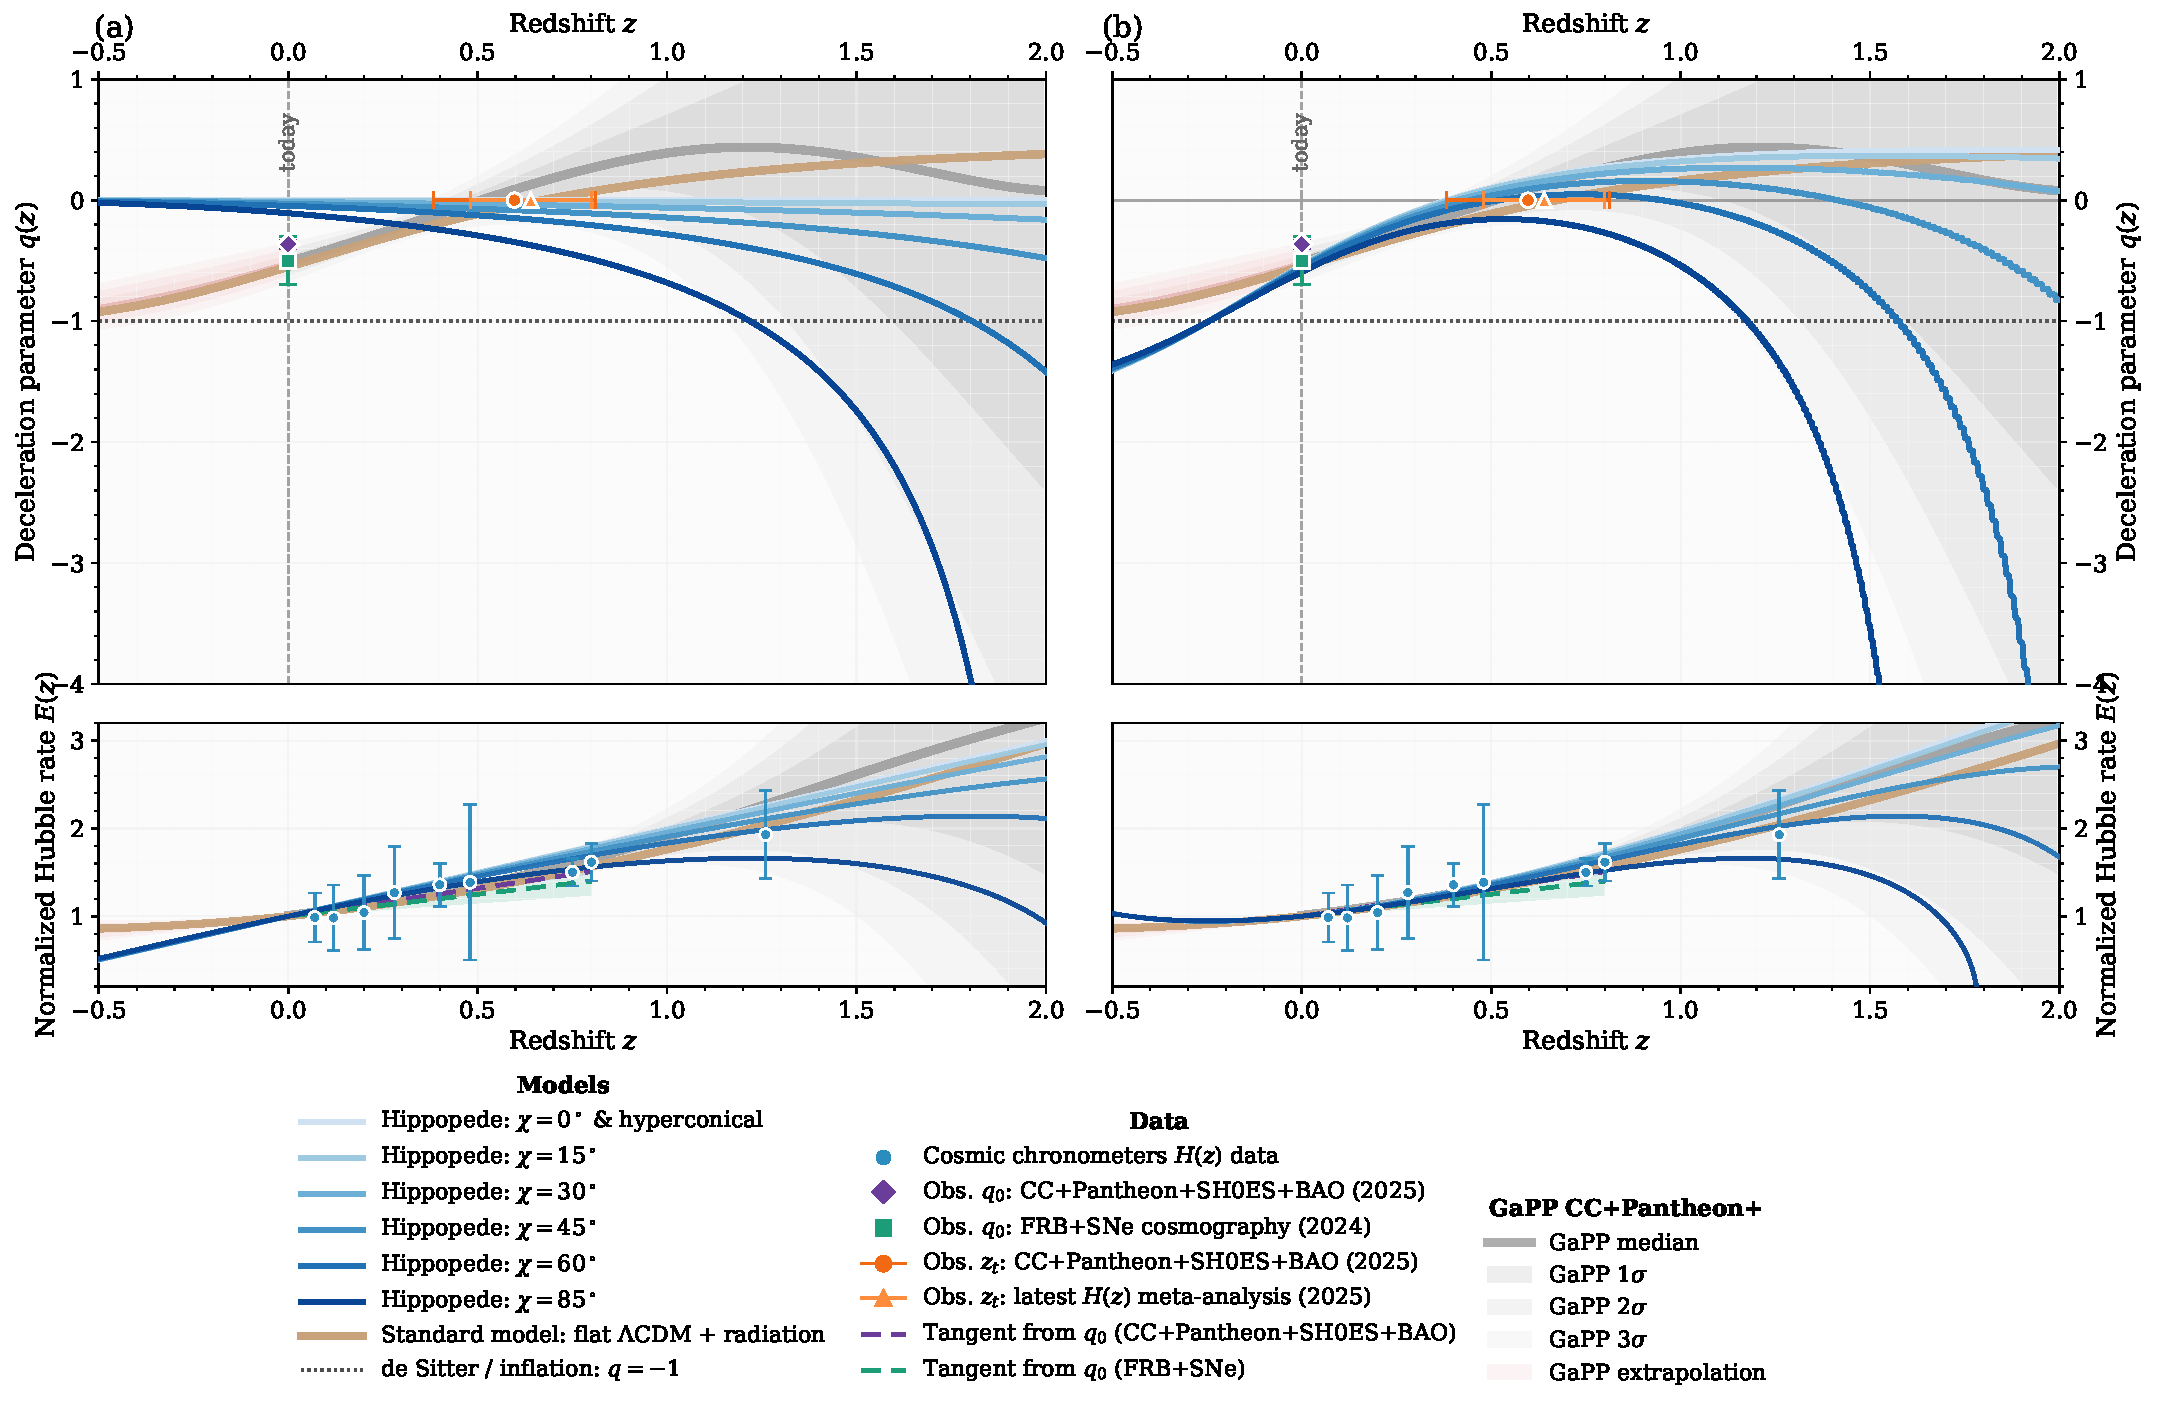
\includegraphics[width=\textwidth]{figures/hippopede_qz_centered_t0_3p0_double_panel_with_gapp}
\caption{
Comparison of the deceleration parameter $q(z)$ (top panels) and normalized expansion rate $E(z)=H(z)/H_0$ (bottom panels) for the centered-scale hippopede simulations (left block) and for the same centered histories after Monjo-type stereographic remapping (right block), both at fixed present time $t_0=3$. The colored curves correspond to the angular sectors $\chi=0^\circ,15^\circ,30^\circ,45^\circ,60^\circ,85^\circ$, while the thick light-brown curve shows the standard flat $\Lambda$CDM$+$radiation background. The upper panels include two present-day estimates of the deceleration parameter, $q_0=-0.364\pm0.032$ from CC+Pantheon+SH0ES+BAO and $q_0=-0.50\pm0.20$ from FRB+SNe cosmography, together with two transition-redshift determinations, $z_t=0.597\pm0.214$ and $z_t=0.64\pm0.16$ \cite{myrzakulov2025q0, gao2024frb, hu2025transition}. The lower panels include normalized cosmic-chronometer data and the GaPP reconstruction band obtained from CC+Pantheon$+$ data with the original Gaussian-process pipeline \cite{seikel2012gapp}. In the projected block the plotted value is $\alpha\simeq0.283$, following the preferred low-redshift implementation of \cite{monjo2018projected}; the Appendix explains why the same family also contains the asymptotic value $\alpha=1/2$ singled out by the radiation-like scaling requirement $H_{\mathrm{perc}}(T)\propto T^2$.}
\label{fig:qz_final}
\end{figure}

\subsection{Observational constraints on the projected model}

Applying the likelihood analysis described above to the DES-SN5YR supernova sample gives $\alpha_{\mathrm{eff}} = 0.323_{-0.012}^{+0.011}\;(1\sigma)$ with the result remaining stable across two independent \texttt{emcee} runs with different stretch-scale choices. Applying the same projected model to the DESI DR1 compressed BAO data gives $\alpha_{\mathrm{eff}} = 0.375_{-0.017}^{+0.016}\; (1\sigma)$, together with best-fit nuisance parameter $\beta = 28.85$ and $\chi^2_{\mathrm{best}}=12.39$ for 10 data points and 2 free parameters. For comparison, a flat $\Lambda$CDM fit with free $\Omega_m$ on the same BAO vector gives $\Omega_m = 0.289$ and $\chi^2_{\mathrm{best}}=11.72$, corresponding to $\Delta \mathrm{AIC}=0.68$. The two models are therefore statistically indistinguishable on the present DESI DR1 compressed BAO compilation.

\purple{Taken together, the supernova and BAO constraints probe distinct effective redshift ranges and remain consistent with a slow increase of the effective projection index relative to the low-redshift reference value $\alpha\simeq0.283$ discussed in \cite{monjo2018projected}.}

\begin{table}[h]
\centering
\color{purple}
\small
\caption{Summary of effective projected-hippopede constraints on $\alpha$.}
\label{tab:alpha_summary}
\begin{tabular}{lll}
\hline
Constraint & Redshift range & $\alpha_{\mathrm{eff}}$ \\
\hline
Low-$z$ projected reference \cite{monjo2018projected} & $z \rightarrow 0$ & 0.283 \\
DES-SN5YR \cite{abbott2024dark} & $0.025$--$1.3$ & $0.323_{-0.012}^{+0.011}$ \\
DESI DR1 BAO \cite{adame2025desi} & $0.295$--$1.491$ & $0.375_{-0.017}^{+0.016}$ \\
\hline
\end{tabular}
\end{table}



%The centered scale factor is defined on the $+u$ branch as $a_c^2=r^2+(u-t)^2$, and the corresponding directional redshift is given by $1+z_\chi=a_{c,\chi}(t_0)/a_{c,\chi}(t)$.

%The limit $\chi=0^\circ$ coincides with the hyperconical reference. The thick light-brown curve shows the standard flat $\Lambda$CDM background with radiation, while the dotted horizontal line marks the de Sitter reference $q=-1$.


At the same time, one should not overstate the analytical control of the projected model. The second-order analytic expansion used in the hyperconical literature is only a local approximation around $z=0$. In practice, the analytic approximation is useful only in a limited neighborhood of the present epoch; for the full displayed interval shown in the figure, the numerical prescription is the relevant one.

A second limitation concerns the interpretation of the projection parameter itself. The value $\alpha\simeq0.283$ gives the best low-redshift phenomenological agreement in the present implementation, but the projected family also contains the asymptotic value $\alpha=1/2$, which is selected by the high-redshift condition that the perceived thermal history satisfies $H_{\mathrm{perc}}(T)\propto T^2$. The two values need not be contradictory: the former can be understood as an effective late-time observational parameter, whereas the latter plays the role of a local/asymptotic physical limit in the sense discussed by Monjo and Campoamor-Stursberg \cite{monjo2020lagrangian, monjo2023hubble}.

\purple{At the purely geometric level, the same appendix also clarifies how the quartic hippopede can be read as a bilobulated deformation of the hyperconical picture, with axial branches that recover the hyperconical $3$-sphere limit and with a possible negative-curvature bilobulated extension described there as a separate geometric generalization rather than as part of the fitted late-time model.}

\blue{The same projected construction also suggests an effective observational isotropization toward high redshift. The anisotropy is clearly visible in the low-redshift dipole-like modulation, but the oblique sectors have a much shorter projected redshift reach than the nearly axial branch, so the observable window is expected to become progressively dominated by the preferred direction at sufficiently early apparent times. Since this point is directly relevant to the BBN-oriented interpretation, we discuss it in more detail in the Appendix.}

\subsubsection{\blue{Interpretation and limitations}}

Centered scale factor provides a cleaner phenomenological bridge between the quartic hypersurface and the asymptotic tangent-sphere picture than the origin-based scale factor. 

\blue{A separate numerical diagnostic indicates that the projected centered histories are indeed close to a dipole-like angular modulation over the low-redshift interval relevant to current background data. Fitting the projected $E(\chi,z)$ curves to the form $E_0(z)[1+D_1(z)\cos\chi]$ over the sectors $\chi=0^\circ$--$85^\circ$ yields $R^2\simeq0.98$--$0.99$ for $0.1\le z\le1$, with fitted amplitudes $D_1\simeq0.006$, $0.024$, $0.055$ and $0.231$ at $z=0.1$, $0.3$, $0.5$ and $1$, respectively. This does not yet constitute a fit to a sky dipole anomaly, because no mapping to an observed celestial direction has been imposed, but it does show that the anisotropy generated by the model is numerically very close to a true dipolar modulation over the late-time window where the observational comparison is performed.}

The present comparison remains exploratory. It is based on a selected set of chronometer and kinematic summary points, not on a full statistical fit, and it depends on a numerical pipeline that includes interpolation, differentiation, branch selection after the first minimum of $a_{c,\chi}(t)$, and, in the projected case, a specific implementation of the Monjo-type remapping. These limitations do not invalidate the qualitative comparison, but they do indicate that any stronger observational claim should be postponed to a dedicated fitting analysis.


\section{Discussion and conclusions}

The hippopede universe is not obtained from a constant-curvature hyperboloid but from a null quadratic relation in an auxiliary ambient (2,4)-spacetime as for an AdS${}_5$ manifold, and the quartic nature of the physical hypersurface arises because the embedding variables depend nonlinearly on the coordinates. In this sense the model should be viewed neither as a standard dS/AdS spacetime nor as a pure hyperconical cone, but rather as an intermediate toy geometry in which the ambient-space quadratic structure survives while the induced 4-dimensional hypersurface acquires a richer anisotropic dynamics.

To avoid a possible misunderstanding, one should emphasize that the toy universe is not identified with the full null hypersurface of the $(2,4)$ ambient space. The latter would be five-dimensional. What is physically relevant here is a four-dimensional submanifold satisfying both the null relation and the angular compatibility condition $u = \rho\cos\chi$, or equivalently the immersed image of the physical variables inside that null hypercone with $u$-axis constraint.

The cleanest way to compare the constructions is to separate three layers. First, the hippopede is recovered from a quartic constraint in Euclidean variables. Second, the toy universe lifts that quartic relation to a $t$-dependent hypersurface in $\mathbb{R}^{1,4}$ whose asymptotic radius is hyperconical-like. Third, after introducing auxiliary coordinates such as $p=(2t\cos\chi,\sin\chi, \vec{\rho}) \in \mathbb{R}^{2,4}$, the same quartic relation is rewritten by constraining the $u$-axis of the null quadratic condition $\|p\|_{\scriptscriptstyle{(2,4)}}^2=0$ in a $(2,4)$-signature ambient space, the same as for an AdS${}_5$ universe. The quartic character of our 4D hippopede universe is therefore not lost; it is encoded in the nonlinear way in which the physical coordinates enter the auxiliary null cone.

In this sense, the dS/AdS hyperboloids, their degenerate null-cone limits, and the hippopede null condition all belong to the same ambient-space family of quadratic loci, although they correspond to different geometric realizations. The relation among them is therefore one of shared embedding structure rather than dynamical equivalence. In fact, the same quartic relation defines a toy expanding geometry whose large-$t$ limit reproduces the linear law associated with hyperconical models, but whose subleading term produces an early-time regularization and a direction-dependent acceleration. The model is best understood as a controlled anisotropic toy universe: simple enough to admit closed analytic expressions, yet nontrivial enough to test how far one can deform exact hyperconical coasting while preserving its large-time behaviour.


%The geometric and cosmological lessons of the construction can be summarized in a compact way. Geometrically, the hippopede furnishes an explicit bridge between a classical quartic curve and the null quadratic constraints familiar from ambient-space relativity. Cosmologically, its four-dimensional extension shows that an asymptotically linear late expansion can coexist with a very different early-time acceleration pattern. 

\section*{\blue{Data Availability}}

\blue{The numerical scripts used to generate the figures are included in the project folder together with the local data files required for the final four-panel comparison figure. In particular, Fig.~\ref{fig:hippopede_growth_3d} is produced by \texttt{plot\_hippopede\_growth\_3d.py}, whereas Fig.~\ref{fig:qz_final} is produced by \texttt{plot\_hippopede\_qz\_double\_panel\_with\_gapp.py}. The supplementary diagnostic script \texttt{analyze\_hippopede\_dipole\_bbn.py} reproduces the late-time dipole-like fit and the constant-$\alpha$ BBN-oriented thermal checks reported in the main text and Appendix, while \texttt{analyze\_hippopede\_variable\_alpha.py} reproduces the running-$\alpha$ scans discussed in the Appendix. The dedicated thermal-history comparison against the standard radiation curve and the observationally inferred BBN corridor is generated by \texttt{plot\_hippopede\_projected\_thermal\_history\_bbn.py}. The bundled data directory contains the curated CC/BAO compilation, the local binned Pantheon$+$ input used by the GaPP reconstruction, and the local copy of the GaPP code needed to reproduce the figure.}

\bibliographystyle{unsrt}
\bibliography{main-hippopede}


\section*{Appendix}

\subsubsection*{Late-epoch linear expansion} 

The description of the hyppopede universe produces an anisotropic acceleration. If one now reads $t$ as a cosmic parameter for the origin-prescription approach and keeps the angular sector $\chi$ fixed, the directional scale factor of this toy model is
\begin{equation}
a_\chi(t):=\rho(t,\chi)=\sqrt{\sin^2\chi+4t^2\cos^2\chi}.
\end{equation}
In this origin-prescription focus, its directional Hubble, acceleration and deceleration functions are then
\begin{equation}
H_\chi(t)=\frac{\dot a_\chi}{a_\chi}=\frac{4t\cos^2\chi}{\sin^2\chi+4t^2\cos^2\chi},
\end{equation}
\begin{equation}
\ddot a_\chi(t)=\frac{4\cos^2\chi\,\sin^2\chi}{\left(\sin^2\chi+4t^2\cos^2\chi\right)^{3/2}},
\end{equation}
\begin{equation}
q_\chi(t):=-\frac{a_\chi\ddot a_\chi}{\dot a_\chi^2}=-\frac{\tan^2\chi}{4t^2}.
\end{equation}
Therefore the model is mildly accelerated for every oblique direction $0<|\chi|<\pi/2$, but the acceleration decays rapidly and
\begin{equation}
H_\chi(t)=\frac{1}{t}+O(t^{-3}),\qquad \ddot a_\chi(t)=\frac{\sin^2\chi}{2|{\cos\chi}|\,t^3}+O(t^{-5}),\qquad q_\chi(t)\to0^-.
\end{equation}
This is the precise sense in which the hippopede universe approaches linear expansion at late times: the asymptotic law is coasting, $a_\chi(t)\sim 2|{\cos\chi}|\,t$, even though the early epoch can display a nonzero positive acceleration. The limiting cases are also transparent: $\chi=0$ gives $a_0(t)=2t$ and hence exact linear expansion for all $t$, while $\chi=\pi/2$ gives $a_{\pi/2}(t)=1$, i.e. no expansion in the purely transverse direction. Numerically, for $\chi=\pi/4$ one finds $q_{\pi/4}(1)=-0.25$, $q_{\pi/4}(2)=-0.0625$, and $q_{\pi/4}(10)=-0.0025$, so the deviation from the linear regime dies off quickly.

\subsubsection*{Early-epoch accelerated universe}



The opposite limit is also informative. For any fixed oblique direction with $\sin\chi\neq0$,
\begin{equation}
a_\chi(0)=|\sin\chi|,\qquad \dot a_\chi(0)=0,\qquad \ddot a_\chi(0)=\frac{4\cos^2\chi}{|\sin\chi|}.
\end{equation}
Since $q_\chi(t)=-\tan^2\chi/(4t^2)$, the deceleration parameter is not merely large near $t=0$; it diverges to $-\infty$ for every fixed oblique direction with $\chi\neq0$. Numerically, for $\chi=\pi/6$ one finds $q_\chi(1)=-0.0833$, $q_\chi(0.5)=-0.333$, and $q_\chi(0.1)=-8.33$, while for $\chi=\pi/4$ the corresponding values are $-0.25$, $-1$, and $-25$. Thus the model becomes extremely accelerated at early times unless one approaches the privileged axis $\chi=0$. If one wishes to compare the toy model with observationally inferred $q(z)$, the next step would be to introduce an effective isotropized scale factor $a_{\mathrm{eff}}(t)$ and then use $1+z=a_{\mathrm{eff}}(t_0)/a_{\mathrm{eff}}(t)$ to map the directional dynamics into redshift space. A dedicated fit is therefore possible, but it requires an additional averaging prescription and should probably be presented separately as a numerical extension rather than as part of the conceptual derivation given here.
Hence the toy universe does not shrink to a point uniformly as $t\to0$: most angular sectors retain a finite initial radius and start with vanishing expansion rate but positive acceleration. The axis $\chi=0$ is singular in this limit, since $a_0(t)=2t$ collapses linearly to zero while the oblique sectors remain finite. This nonuniform behaviour is another sign that the model should be read as a biaxial toy geometry rather than as a realistic isotropic cosmology.


\subsubsection*{Bilobulated interpretation, axial hyperconical limit, and a possible $K=-1$ extension}

The large-$t$ geometry of the quartic model is best interpreted in two complementary ways. In the origin-based description one has
\begin{equation}
\rho(t,\chi)=\sqrt{\sin^2\chi+4t^2\cos^2\chi}
=2|{\cos\chi}|\,t+\frac{\sin^2\chi}{4|{\cos\chi}|\,t}+O(t^{-3}),
\end{equation}
so the leading term reproduces the dipolar law of the two tangent $3$-spheres discussed in the main text. Since the hyperconical universe of Monjo is foliated by spatial $3$-spheres of radius proportional to $t$, this is the precise sense in which each axial branch of the hippopede approaches a hyperconical branch at late times. Along the preferred directions $\chi\approx0$ and $\chi\approx\pi$, the quartic model therefore recovers the same linear coasting behaviour as the hyperconical construction, while the oblique sectors retain the anisotropic correction encoded in the subleading term.

The centered description clarifies the geometry of each individual lobe. On the $+u$ branch we defined
\begin{equation}
a_{c,\chi}(t):=\sqrt{r^2+(u-t)^2}
=\sqrt{\rho(t,\chi)^2+t^2-2t\,\rho(t,\chi)\cos\chi}.
\end{equation}
Using the same large-$t$ expansion for $\rho(t,\chi)$ one finds
\begin{equation}
a_{c,\chi}(t)^2
=t^2+\frac{\sin^2\chi}{2}+O(t^{-2}),
\qquad
a_{c,\chi}(t)
=t+\frac{\sin^2\chi}{4t}+O(t^{-3}).
\end{equation}
Thus, when each branch is viewed from the center of curvature of its own asymptotic tangent sphere, the lobe tends to a linearly expanding spatial $3$-sphere. This is again compatible with the hyperconical picture, because the constant-time spatial sections of the latter are themselves $3$-spheres. The difference is therefore mainly one of viewpoint: the origin-based picture emphasizes the dipolar two-branch structure, whereas the centered picture emphasizes the local recovery of a single hyperconical lobe.

This also shows why the bilobulated interpretation is close to, but not identical with, the quartic hippopede. The neck joining the two asymptotic lobes is certainly the most visible new geometric feature, but it is not the only one. Away from the strict large-$t$ limit the quartic relation leaves a residual angular deformation throughout the profile, and this is precisely what produces the anisotropic correction
\begin{equation}
\rho(t,\chi)-2|{\cos\chi}|\,t
=\frac{\sin^2\chi}{4|{\cos\chi}|\,t}+O(t^{-3}).
\end{equation}
In that sense, the hippopede should be viewed as a bilobulated hyperconical deformation: the neck expresses the global two-lobe topology, while the quartic angular term controls how the geometry departs from a pair of exact hyperconical branches at finite $t$.

The same intuition suggests a natural negative-curvature extension, although this goes beyond the exact quartic model studied in the main text. One may consider a compact hyperbolic $3$-manifold $N$ with totally geodesic boundary $\partial N\cong\Sigma_g$, where $\Sigma_g$ is a closed surface of genus $g\ge2$, and form the double
\begin{equation}
M_g=N\cup_{\phi}\bar N,
\end{equation}
with $\phi:\Sigma_g\to\Sigma_g$ an orientation-reversing boundary isometry. The resulting closed manifold carries a smooth metric of constant sectional curvature $K=-1$ and provides a mathematically natural bilobulated space with a geodesic neck. A cosmological line element of the form
\begin{equation}
ds^2=-dt^2+a(t)^2 h_{ij}dx^i dx^j,
\end{equation}
with $h_{ij}$ the hyperbolic metric on $M_g$, then defines a negatively curved FRW-type extension of the same bilobulated intuition.

However, this $K=-1$ construction should be interpreted carefully. The standard geodesic-polar expression
\begin{equation}
d\ell^2=d\rho^2+\sinh^2\rho\,d\Omega_2^2
\end{equation}
describes the simply connected space $H^3$ around a chosen point, not the full global geometry of a compact double $M_g$. Likewise, the quartic hippopede relation is not literally recovered as a global section of an arbitrary hyperbolic double. The connection is therefore structural rather than exact: the quartic model provides the explicit anisotropic toy geometry studied in this paper, whereas the doubled hyperbolic manifolds furnish a natural family of bilobulated negative-curvature analogues in which the neck is global and the asymptotic hyperconical intuition is replaced by hyperbolic ends or local axial neighbourhoods. The present work establishes the former rigorously and leaves the latter as a plausible geometric extension for future study.


\subsubsection*{Projected thermal asymptotics and the BBN-motivated limit $\alpha=1/2$}

To discuss primordial nucleosynthesis in the projected picture, one must distinguish between the intrinsic geometric time and the perceived thermal history of the projected radiation sector. The latter is the relevant quantity for BBN. Assuming the minimal adiabatic identification $T_{\mathrm{perc}}\propto 1+z$ (up to the usual slowly varying entropy factor $g_{*S}$), the high-redshift behaviour of the projected Hubble function follows directly from the asymptotics of the Monjo-type projection.

For $k=1$ one has $x_{\max}=\sqrt{3}/2$ and $b(x)=\sqrt{1-x^2}$, with $b(x_{\max})=1/2$. Writing $x=x_{\max}-\delta$ with $\delta\downarrow0$, one finds
\begin{equation}
2b-1\;=\;2\sqrt{1-x^2}-1\;=\;-2\sqrt{3}\,\delta+O(\delta^2),
\end{equation}
while
\begin{equation}
\sqrt{1-(1-b)^2}=\sqrt{2b-b^2}=\frac{\sqrt{3}}{2}+O(\delta).
\end{equation}
Therefore the line-of-sight integrand behaves as
\begin{equation}
\frac{\sqrt{1-(1-b)^2}}{b[2(b-1)+1]}
\;=\; -\frac{1}{2\delta}+O(1),
\end{equation}
so that
\begin{equation}
\xi_1(x)= -\frac12\ln\delta + O(1).
\end{equation}
Since $\xi_1(x)=\ln(1+z)$, this implies the boundary relation
\begin{equation}
\delta=x_{\max}-x(z)\propto (1+z)^{-2}.
\end{equation}

Now define $\eta:=\gamma_0-\gamma(x)$. Because $\gamma'(x)=1/\sqrt{1-x^2}$ is finite at $x=x_{\max}$, one has $\eta\propto\delta$. Near the boundary, the Monjo-type projection
\begin{equation}
f_{\hat r}^{\alpha}(x)=2\arctan\!\left[\frac{\gamma(x)/2}{(1-\gamma(x)/\gamma_U)^\alpha}\right]
\end{equation}
obeys
\begin{equation}
\frac{df_{\hat r}^{\alpha}}{dx}\propto \eta^{\alpha-1}\propto \delta^{\alpha-1}.
\end{equation}
Combining this with $dx/dz\propto (1+z)^{-3}$ gives
\begin{equation}
\frac{d\hat r}{dz}\propto (1+z)^{-(1+2\alpha)},
\qquad
\hat H(z)=\left(\frac{d\hat r}{dz}\right)^{-1}\propto (1+z)^{1+2\alpha}.
\end{equation}
Hence the projected family satisfies the asymptotic law
\begin{equation}
E_{\mathrm{hyp}}^{\mathrm{proj}}(z)\propto (1+z)^n,
\qquad n=1+2\alpha.
\end{equation}
Under the perceived thermal identification $T_{\mathrm{perc}}\propto 1+z$, this becomes
\begin{equation}
H_{\mathrm{perc}}(T)\propto T^{1+2\alpha}.
\end{equation}
The radiation-dominated standard law $H(T)\propto T^2$ is therefore recovered precisely when
\begin{equation}
\alpha=\frac12.
\end{equation}

\blue{The asymptotic exponent, however, is only part of the BBN requirement. A direct numerical calibration of the same projected prescription, performed with the extended lookup implemented in \texttt{analyze\_hippopede\_dipole\_bbn.py}, gives $n_{\mathrm{eff}}=1.999999$ over the interval $10^3\lesssim z\lesssim10^6$, as expected for $\alpha=1/2$, but the corresponding physical normalization obtained from $H_{\mathrm{perc}}(T)=H_0E_{\mathrm{hyp}}^{\mathrm{proj}}(T/T_0-1)$ is still too large by an approximately constant factor $H_{\mathrm{perc}}/H_{\mathrm{rad}}\simeq10.2$ in the representative BBN temperature range $T\simeq0.07$--$1\,\mathrm{MeV}$ when compared with the standard radiation-era law. Thus the constant-$\alpha$ branch with $\alpha=1/2$ reproduces the correct $T^2$ scaling but not yet the standard normalization.}

\blue{This observation motivates a second, more flexible numerical test within the same projected family: instead of identifying a single constant projection index, one may allow a smooth perceived-history interpolation}
\begin{equation}
\blue{
\alpha(z)=\alpha_{\mathrm{low}}+\frac{\alpha_{\mathrm{high}}-\alpha_{\mathrm{low}}}{2}
\left[
1+\tanh\!\left(
\frac{\ln(1+z)-\ln(1+z_c)}{2}
\right)
\right],
}
\end{equation}
\blue{with $\alpha_{\mathrm{low}}=0.283$ fixed by the successful low-redshift phenomenology of Fig.~\ref{fig:qz_final}, and $\alpha_{\mathrm{high}}=1/2$ fixed by the radiation-like asymptotic requirement. Exploratory scans with the supplementary script \texttt{analyze\_hippopede\_variable\_alpha.py}, checked directly against the literal projected-map relation $H_{\mathrm{perc}}(T)=H_0E_{\mathrm{hyp}}^{\mathrm{proj}}(T/T_0-1)$, show that the most promising BBN-like window is obtained for an earlier and narrower transition, approximately around}
\begin{equation}
\blue{
z_c\sim 1.6\times10^4
}
\end{equation}
\blue{This choice preserves the low-redshift sector almost unchanged, since $\alpha(1)\simeq0.28302$ and $\alpha(2)\simeq0.28303$, while driving the projected thermal history very close to the standard radiation-era normalization across the BBN window. In the updated diagnostic we compare it directly with the observationally inferred BBN corridor obtained from the 2024 primordial-abundance fit $\Delta N_{\mathrm{eff}}=-0.10\pm0.21$ of \cite{schoneberg2024bbn}. A representative near-optimal case is}
\begin{equation}
\blue{
z_c=1.616\times10^4
}
\end{equation}
\blue{for which the geometric-mean normalization with respect to the standard radiation curve over the interval $T\simeq0.07$--$1\,\mathrm{MeV}$ is}
\begin{equation}
\blue{
\left\langle \frac{H_{\mathrm{perc}}}{H_{\mathrm{rad}}}\right\rangle_{\mathrm{geom}}
\simeq 0.9915,
}
\end{equation}
\blue{with pointwise values}
\begin{equation}
\blue{
\frac{H_{\mathrm{perc}}}{H_{\mathrm{rad}}}\approx
0.991,\ 0.992,\ 0.993,\ 0.991,\ 0.991
}
\end{equation}
\blue{at $T=0.07,\ 0.10,\ 0.20,\ 0.50,\ 1.0\,\mathrm{MeV}$, respectively. Relative to the BBN-inferred central history of \cite{schoneberg2024bbn}, the corresponding residuals are only $-1.2\times10^{-3},\ 4.0\times10^{-4},\ 1.0\times10^{-3},\ -1.2\times10^{-3},\ -6.3\times10^{-4}$ over the same five temperatures. In the plotted diagnostic these values are read from the same literal projected-map evaluation after the mild log-space smoothing mentioned above, which removes small non-physical spikes produced by numerical differentiation of the dense lookup table without changing the BBN-window normalization in any material way. In other words, the same projected family admits a smooth perceived thermal history for which the whole BBN window is brought extremely close not only to the standard radiation background, but also to the currently inferred observational BBN corridor, rather than remaining strongly suppressed in the low-redshift constant-$\alpha$ branch or enhanced by more than one order of magnitude in the pure $\alpha=1/2$ branch.}

\blue{This does not yet amount to a full light-element calculation, and we therefore do not claim in this paper that the primordial abundances are already reproduced in detail. Nevertheless, the numerical result is strong enough to support a more focused statement: within the projected-hyperconical interpretation, the apparent thermal history can be made quantitatively compatible with both the normalization and the asymptotic $T^2$ scaling expected for a BBN-like radiation era, provided one allows a smooth transition from the low-redshift phenomenological value $\alpha\simeq0.283$ to the asymptotic physical value $\alpha=1/2$. A complete BBN claim would then require the next layer of analysis, namely a consistent treatment of $g_{*S}(T)$, the weak-interaction freeze-out, and the light-element reaction network.}

\blue{The same numerical exploration clarifies how the inherited anisotropy enters the projected early-time discussion. If one tries to construct a genuinely sector-dependent quantity}
\begin{equation}
\blue{
R_\chi(T):=\frac{H_{\chi,\mathrm{perc}}(T)}{H_{\mathrm{rad}}(T)},
}
\end{equation}
\blue{using the projected centered histories themselves, one finds that each fixed angle $\chi$ has only a finite internal redshift support. For the centered branches adopted in this work, the maximum unprojected redshifts are approximately}
\begin{equation}
\blue{
z^*_{\max}\simeq 3.0\times10^4,\ 12.36,\ 5.87,\ 3.78,\ 2.80,\ 2.13
}
\end{equation}
\blue{for $\chi=0^\circ$, $15^\circ$, $30^\circ$, $45^\circ$, $60^\circ$ and $85^\circ$, respectively. When these endpoints are translated back through the common projected-hyperconical map with $\alpha=1/2$, they correspond only to}
\begin{equation}
\blue{
z_{\mathrm{obs},\max}\simeq 422,\ 7.64,\ 5.01,\ 3.87,\ 3.23,\ 2.74,
}
\end{equation}
\blue{or, equivalently, to perceived temperatures of order}
\begin{equation}
\blue{
T_{\max}\simeq 9.9\times10^{-8},\ 2.0\times10^{-9},\ 1.4\times10^{-9},\ 1.1\times10^{-9},\ 1.0\times10^{-9},\ 8.8\times10^{-10}\ \mathrm{MeV}.
}
\end{equation}
\blue{These scales lie far below the standard BBN window $T\sim0.07$--$1\,\mathrm{MeV}$. Therefore the present centered branch does not yet provide a full anisotropic BBN calculation sector by sector: the oblique projected histories simply terminate long before one reaches the redshifts relevant to primordial nucleosynthesis.}

\blue{This is nevertheless physically informative. It means that the stereographic remapping does not erase the underlying anisotropy, but it does strongly filter its observational visibility. The oblique sectors dominate the low-redshift phenomenology and are responsible for the dipole-like modulation discussed in the main text, whereas at sufficiently high apparent redshift the observer progressively loses access to those sectors and is left mainly with the nearly axial branch. In that sense the projected model suggests an effective observational isotropization toward high redshift: the background remains intrinsically anisotropic, yet the observable radiation history becomes increasingly dominated by the preferred direction. The running-$\alpha$ BBN-like result obtained above should therefore be interpreted as an effective perceived thermal history of the projected radiation sector, not as a complete primordial-nucleosynthesis solution on the anisotropic centered background itself.}

\end{document}




===== REMOTE OVERLEAF VERSION =====
\documentclass[11pt]{article}

\usepackage{amsmath,amssymb,amsfonts}
\usepackage{xcolor}
\usepackage{authblk}
\usepackage{geometry}
\usepackage{graphicx}
\usepackage{hyperref}
\usepackage{chngcntr}
\geometry{margin=1in}
\graphicspath{{figures/}}
\DeclareGraphicsExtensions{.pdf,.png,.jpg}
\renewcommand{\vec}[1]{\boldsymbol{#1}}
\newcommand{\blue}[1]{{\color{blue}#1}}
\newcommand{\purple}[1]{\textcolor{purple}{#1}} 
\newcommand{\red}[1]{{\color{red}#1}}
\renewcommand\Authfont{\normalsize}
\renewcommand\Affilfont{\small}
\counterwithout{table}{section}
\renewcommand{\thetable}{\arabic{table}}

\title{Hippopede Universe as a toy model of late-linear expansion}
\author[1,2]{Robert Monjo}
\author[3]{Manel Romero}
\author[4]{Ardra E. Sasi}
\affil[1]{Department of Mathematics, CUNEF University, Calle Almansa 101, Madrid 28040, Spain}
\affil[2]{Centro de Estudios Cosmologicos ``Prof. Jaime Roessler Bonzi'', Facultad de Ciencias, Universidad de Chile, Las Palmeras 3425, \~Nunoa, Santiago 7750000, Chile}
\affil[3]{Area of Chemistry, University of Barcelona, Campus Diagonal: Av. Joan XXIII, 27-31, 08028 Barcelona, Spain}
\affil[4]{School of Pure and Applied Physics
Mahatma Gandhi University, Priyadarsini Hills P.O. Athirampuzha, Kottayam, Kerala 686560, India}
\date{}

\begin{document}

\maketitle

\begin{abstract}

The hippopede is a classical quartic curve with a long history in geometry, yet it also offers a suggestive reinterpretation in modern embedding approaches. In this work we show that its defining relation can be recast as a null quadratic constraint in an auxiliary pseudo-Euclidean space, thereby placing the extended hippopede hypersurface in direct analogy with the ambient-space constructions commonly used for de Sitter and anti de Sitter geometries. We then apply the same quartic structure to a four-dimensional toy universe whose large-$t$ limit consists of two tangent $3$-spheres, so that the model becomes a simple laboratory for asking whether a hyperconical late-time coasting law can emerge together with a distinct early-time acceleration.

\end{abstract}

\section{Introduction}

\subsection{Motivation}

Model-dependent probes such as BAO and CMB fits, and more direct determinations based on cosmic chronometers (CC) and Type Ia supernovae (SNe Ia), do not always favour the same late-time expansion history. This discrepancy is visible both in the local Hubble tension and in the broader discussion of how background expansion should be inferred from intrinsic versus projection-dependent observables. In hyperconical approaches this distinction is especially relevant, because an apparently accelerated phenomenology can arise from the projection map even when the underlying ambient-space expansion remains asymptotically linear \cite{monjo2018projected, monjo2023hubble}.

A natural starting point for the present work is the long-standing interest in coasting cosmologies, namely models for which the late-time scale factor behaves approximately as $a(t)\propto t$. Such scenarios were studied early on by John et al. \cite{john2000coasting, John2019} as viable alternatives to standard decelerating or accelerated backgrounds, and more recently they have reappeared in hyperconical modified-gravity constructions where the linear law is tied to an ambient-space geometric constraint \cite{monjo2017hyperconical, Monjo_2024, Monjo_2025}. Within that framework, recent astrophysical tests indicate that the model can remain phenomenologically competitive beyond galactic rotation curves: hydrostatic-equilibrium analyses of X-COP clusters show good agreement in hot-gas-dominated regions beyond $\sim1\,\mathrm{Mpc}$, while galaxy--galaxy weak-lensing reconstructions yield flat circular velocities on megaparsec scales that compare favorably with MOND in the same regime \cite{monjo2025clusters, monjo2025lensing}.

The main cosmological motivation for relaxing exact coasting at all epochs comes from primordial nucleosynthesis. In a strictly linear expansion, $H(t)=1/t$, the Universe remains older at a fixed temperature than in the standard radiation-dominated scenario, so weak interactions stay effective for longer and the neutron-to-proton ratio freezes out under different conditions. This alters the synthesis window for light nuclei: in particular, it tends to overproduce helium and strongly affects deuterium survival unless additional assumptions are introduced \cite{sethi1999coasting, dev2002coasting}. For that reason, even if a late coasting regime is phenomenologically attractive, one is naturally led to explore toy geometries in which the large-$t$ behaviour remains asymptotically linear while the early-time acceleration differs from zero. The hippopede universe proposed below is meant precisely in that spirit: it is not offered as a realistic cosmology, but as a controllable biaxial toy model interpolating between a regular quartic geometry and a hyperconical-like late regime.

\subsection{Hippopede curve}
Algebraic curves of low degree have long played a role not only in classical geometry but also in astronomical modelling and, more recently, in modern theoretical physics. Among these curves, the \emph{hippopede} occupies a historically interesting position. The curve was already known in Greek geometry and is traditionally associated with the work of Eudoxus and later commentators such as Proclus, appearing in discussions of planetary motion and spherical constructions \cite{Gregory_2011, Taub2020, BotteriCasazza2023}. In modern mathematical terminology, the hippopede is a quartic plane curve that can be written in implicit form as the set of points $(x,y) \in \mathbb{R}^2$ satisfying:
\begin{equation}
    k x^2 + y^2 - (x^2+y^2)^2 = 0
\end{equation}
where $(x,y)$ are the Cartesian coordinates and $k > 0$ is a positive real constant.


The geometry of this curve and related quartic curves has been discussed in classical works on plane algebraic curves and in modern mathematical treatments of special curves. Standard references include the classical monograph of Lawrence \cite{lawrence1972catalogue} and more recent surveys of plane quartics such as those by Gibson \cite{gibson2001elementary}. From the viewpoint of differential geometry, the curve can also be viewed as a deformation of the circle controlled by the parameter $k$. Writing $k=4t^2$ and introducing polar coordinates $(r,\theta)$ defined by $x=r\cos\theta$ and $y=r\sin\theta$, the defining equation becomes $r^2 = 4t^2\cos^2\theta + \sin^2\theta$. This representation shows that the curve can be regarded as a deformation of the circle in which the radial coordinate depends on the polar angle. When $t=\tfrac12$ (equivalently $k=1$) the curve reduces to the unit circle. For $t >\tfrac12$ the curve develops the characteristic shape of the hippopede, elongated along the horizontal axis.

From the algebraic viewpoint the curve is a quartic plane curve symmetric under reflections across both coordinate axes. Its intersection with the coordinate axes is easily determined: the curve passes through $(0,\pm1)$ independently of the value of $k$, while its intersection with the horizontal axis occurs at $(\pm 2t,0)$. These properties make the hippopede a particularly simple example of a quartic curve whose geometry is controlled by a single parameter.

\subsection{Hyperconical, \textit{de Sitter} and \textit{anti de Sitter} geometries}

The hyperconical universe $\mathcal{H}^4$ is mathematically defined as the null hypersurface embedded in a pseudo-Euclidean manifold (flat ambient space) of signature $s=(1,4)$ or $s=(4,1)$, which is usually referred to as 5-dimensional Minkowskian spacetime $\mathbb{R}^s$ \cite{monjo2017hyperconical, Monjo_2024}. For instance, the $(4,1)$ convention can be written as follows:
\begin{equation}
\mathcal{H}^4:=\left\{q=(t,\vec{\rho})\in\mathbb{R}^{4,1}\;:\;-t^2+\|\vec{\rho}\|_{\scriptscriptstyle{(4,0)}}^2=0\right\},
\end{equation}where $\|\vec{\rho}\|_{\scriptscriptstyle{(4,0)}} ^2$ represents the quadratic form of $\vec{\rho} = (x,y,z,u)$ in $\mathbb{R}^4$, that is, $\|\vec{\rho}\|_{\scriptscriptstyle{(4,0)}} ^2 = x^2+y^2+z^2+u^2$. Equivalently, on each constant-$t$ slice one has $\|\vec{\rho}\|_{\scriptscriptstyle{(4,0)}} =t$, so the spatial section is a 3-sphere of radius $t$ and the resulting background expands linearly. By contrast, the 4-dimensional de Sitter (dS${}_4$) spacetime is described by the hyperboloid $-X_0^2+X_1^2+X_2^2+X_3^2+X_4^2=\alpha^2$ in the same ambient-space $\mathbb{R}^{4,1} \ni (X_0, \dots X_4) = X$, but with nonzero curvature radius $\alpha = \|X\|_{\scriptscriptstyle{(4,1)}}$. Within this embedding picture, the hyperconical universe may be regarded as the degenerate limit $\alpha\to0$ of the dS${}_4$ family, for which the regular hyperboloid collapses to the null cone. It is therefore better described as a singular limit of dS geometry than as an ordinary dS spacetime. 

Finally, a $4$-dimensional \textit{anti de Sitter} (AdS${}_4$) spacetime is a pseudo-Riemannian manifold embedded by increasing up to two time coordinates $(t_1, t_2)$, which satisfy $-t_1^2-t_2^2+X_1^2+X_2^2+X_3^2 = - \alpha$ in a pseudo-Euclidean space $\mathbb{R}^{3,2}$ with signature $(3,2)$.  Thse constructions provide a powerful geometric representation of constant curvature cosmological spacetimes and is standard in the literature on relativistic cosmology and quantum field theory in curved spacetime \cite{hawking1973large, spradlin2001les}.

What these constructions share is the quadratic embedding language, and this is exactly the bridge on which the present toy model is built. The hippopede extension sits between both pictures: like the hyperconical case, it has an asymptotically linear radius; like the dS/AdS constructions, it is most naturally understood through a higher-dimensional quadratic relation. Hyperconical models have been proposed precisely because they realize a linear late expansion law in a natural embedding setting \cite{monjo2017hyperconical}. It is therefore natural to ask whether nearby toy models can preserve the asymptotic coasting behaviour $a(t)\propto t$ while allowing a different acceleration pattern during early epochs. The higher--dimensional hippopede provides a minimal laboratory for that question: it keeps the same large-$t$ linear scaling along the expanding directions, but it regularizes the exact hyperconical behaviour by a finite angular term that modifies the early dynamics.


The logic of the paper is therefore fourfold: first, we identify the correct high--dimensional extension of the quartic relation; second, we extract its large-$t$ limit as two tangent hyperspheres, with the intention of a hyperconical toy universe; third, we compute the corresponding directional Hubble and acceleration functions; and fourth, we relate the resulting quartic toy model to the ambient-space construction used for dS/AdS geometries.


\section{Data and Methods}

\subsection{Data}

We used observed estimates of the deceleration parameter collected from: i) the present deceleration estimates $q_0=-0.364\pm0.032$ together with the transition redshift estimate $z_t=0.597\pm0.214$ from the combined CC+Pantheon+SH0ES+BAO analysis \cite{myrzakulov2025q0}; ii) the cosmographic estimate $q_0=-0.50\pm0.20$ obtained from fast radio bursts (FRB) combined with supernovae (SNe) in \cite{gao2024frb}; iii) the screened meta-analytic transition estimate $z_t=0.64\pm0.16$ from the latest $H(z)$ compilation analysis of \cite{hu2025transition}. Moreover, observed estimates of normalized Hubble factor $E_{\mathrm{obs}}(z)=H(z)/H_0$ were computed from the CC measurements, with $H_0=70~\mathrm{km\,s^{-1}\,Mpc^{-1}}$ (Table \ref{tab:cc_data_figures}).

For the dedicated low-to-intermediate redshift constraints on the projected model, we additionally use two complementary datasets. The DES-SN5YR Type Ia supernova sample \cite{abbott2024dark} contains 1829 supernovae over the interval $0.025 \le z \le 1.3$. The compressed DESI DR1 baryon acoustic oscillation catalogue \cite{adame2025desi} provides measurements of $D_M/r_s$, $D_H/r_s$, and $D_V/r_s$ in six galaxy and quasar tracer bins centered at $z_{\rm eff}=0.295$, $0.510$, $0.706$, $0.930$, $1.317$, and $1.491$. In this first geometric analysis we exclude the Ly$\alpha$ forest point near $z_{\rm eff}\simeq2.33$, so that the fit remains restricted to the lower-redshift window most directly comparable with the supernova sector.

\begin{table}[h]
\centering
\small
\caption{Observational inputs used in this work.}
\label{tab:dataset_summary}
\begin{tabular}{lll}
\hline
Redshift range & Observable(s) & Dataset \\
\hline
local to intermediate & $q_0$, $z_t$ & Cosmographic constraint \cite{myrzakulov2025q0,gao2024frb,hu2025transition} \\
$0.07$--$1.26$ & $H(z)$, hence $E(z)=H/H_0$ & Cosmic chronometers \\
low to intermediate & reconstructed $q(z)$ and $E(z)$ & CC+Pantheon$+$ GaPP \cite{seikel2012gapp} \\
$0.025$--$1.3$ & SN distance moduli & *DES-SN5YR \cite{abbott2024dark} \\
$0.295$--$1.491$ & $D_M/r_s$, $D_H/r_s$, $D_V/r_s$ & *DESI DR1 BAO \cite{adame2025desi} \\
\hline
\end{tabular}
\end{table}

Note:  *Likelihood constraint on $\alpha_{\mathrm{eff}}$

\begin{table}[h]
\label{tab:cc_data_figures}
\centering
\small

\caption{Observed values of the Hubble parameter according to the cosmic chronometers considered.}

\begin{tabular}{lll}
\hline
$z$ & $H(z)$ [km s$^{-1}$ Mpc$^{-1}$] & Source \\
\hline
0.07, 0.12, 0.20, 0.28 & 69.0$\pm$19.6,\;68.6$\pm$26.2,\;72.9$\pm$29.6,\;88.8$\pm$36.6 & Zhang et al. \cite{zhang2014hubble} \\
0.40, 0.48 & 95.0$\pm$17.0,\;97.0$\pm$62.0 & Stern et al. \cite{stern2010chronometers} \\
0.75 & 105.0$\pm$7.9(stat)$\pm$7.3(sys) & Jimenez et al. \cite{jimenez2023photometry} \\
0.80 & 113.1$\pm$15.1(stat)$^{+29.1}_{-11.3}$(sys) & Jiao et al. \cite{jiao2023legac} \\
1.26 & 135.0$\pm$35.0 & Tomasetti et al. \cite{tomasetti2023vandels} \\
\hline
\end{tabular}


\end{table}

Finally, Gaussian-process reconstructions obtained with the original GaPP logic are included in order to compare the centered hippopede histories with model-independent reconstructions of both $q(z)$ and $E(z)$ based on CC+Pantheon$+$ data \cite{seikel2012gapp}.



\subsection{Model}

\subsubsection{The coasting hippopede universe}

Let $(t, \vec \rho) = (t,x,y,z,u)\in\mathbb{R}^{1,4}$, and consider the hypersurface
\begin{equation}
\label{eq:hippopede_univ}
 x^2 + y^2 + z^2 + 4t^2 u^2 = (x^2 + y^2 + z^2 + u^2)^2 .
\end{equation}
defined as an upper-dimensional extension of the hippopede curve.

 Let $\rho^2 := \|\vec \rho\|_{\scriptscriptstyle{(4,0)}}^2$ with $\|\vec \rho\|_{\scriptscriptstyle{(4,0)}}^2=x^2 + y^2+z^2 + u^2 =: r^2 + u^2$ and introduce spherical coordinates around the distinguished $u$-axis,
\begin{equation}\label{eq:angle-constraint}
u=\rho\cos\chi,\qquad r=\rho\sin\chi.
\end{equation}
Then Eq.~\eqref{eq:hippopede_univ} becomes
\begin{equation}
\label{eq:hippopede_univ2}
\rho^2=\sin^2\chi+4t^2\cos^2\chi.
\end{equation}
Introducing the auxiliary coordinates
$t_1:=2t\cos\chi,\; t_2:=\sin\chi$,
the same relation is exactly equivalent to the null condition $\vec{\rho}^2-t_1^2-t_2^2=0$,
in a 6D ambient space with pseudo-Euclidean metric of signature $(2,4)$ or $(4,2)$. According to Eq. \ref{eq:angle-constraint}, the 4D hippopede hypersurface is therefore given by the dipolar-angle constraint $u^2-{\vec \rho}^2(1-t_2^2) = 0$ of the 6D null hypercone in the ambient space, where $u$ is the fourth coordinate of $\vec \rho$. This is the minimal consistent immersion formulation of the toy model, which is equivalent to encode the quartic hypersurface through a nonlinear map from the physical variables $(t,\chi)$ into an auxiliary null cone (Eq. \ref{eq:hippopede_univ2}). This exact expression already displays two key points: i) it contrasts with the \textit{light cone} $\{p = (t,\vec{\rho}) \in \mathbb{R}^{1,4}\;:\; \|p\|^2 = 0\}$ defined in the $(1,4)$-signature hyperconical universe; ii) along every direction with $\cos\chi\neq0$, the size of the configuration grows linearly with $t$ for large times, as in the $\mathbb{R}^{1,4}$ case. More precisely,
\begin{equation}
\rho(t,\chi)=2|{\cos\chi}|\,t+\frac{\sin^2\chi}{4|{\cos\chi}|\,t}+O(t^{-3})\qquad (t\to\infty).
\end{equation}
The leading term
\begin{equation}
\rho_{\infty}(t,\chi)=2|{\cos\chi}|\,t
\end{equation}
is exactly the dipolar equation of the union of the two tangent $3$-spheres
\begin{equation}
x^2+y^2+z^2+(u-t)^2=t^2,\qquad x^2+y^2+z^2+(u+t)^2=t^2.
\end{equation}
Indeed, each sphere of radius $t$ centered at $u=\pm t$ satisfies $\rho=2t|\cos\chi|$. In this sense the quartic hypersurface interpolates between a smooth finite-$t$ geometry and a double-sphere large-$t$ limit, which is the natural place to import the hyperconical-universe intuition into the hippopede setting.

At the purely geometric level, the most immediate ``origin-based'' reading of the quartic hypersurface is simply $a_{\chi}(t):=\rho(t,\chi)$.  If one now reads $t$ as a cosmic parameter and keeps the angular sector $\chi$ fixed, the directional scale factor of this toy model is
\begin{equation}
a_\chi(t):=\rho(t,\chi)=\sqrt{\sin^2\chi+4t^2\cos^2\chi}.
\end{equation}
Its directional Hubble $H_\chi(t)= \dot a_\chi / a_\chi$ and acceleration $\ddot a_\chi(t)$ determine its deceleration function as $q_\chi(t):= - a_\chi\ddot a_\chi / \dot a_\chi^2 = - a_\chi a_\chi\ddot / H_\chi(t)^2$. We remark on that prescription because it yields closed analytic expressions and provides a useful first contrast with the hyperconical case with pure linear expansion (see Appendix). However, the numerical results eventually adopted for the two definitive comparison figures are based instead on a centered effective scale factor measured with respect to the center of curvature of one asymptotic tangent branch.

\begin{figure}[t]
\centering

\includegraphics[width=0.78\textwidth]{hippopede_growth_3d}
\caption{Three-dimensional visualization of the nested hippopede hypersurfaces associated with increasing values (0.5, 1, 2 and 3.0) of the parameter $t$. The distinguished axis is $u$, while the orthogonal directions are represented through $(\sqrt{x^2+y^2},z)$. As $t$ grows, the quartic hypersurface approaches the large-time limit formed by two tangent 3-spheres centered at $u=\pm t$, making explicit the emergence of an asymptotically hyperconical coasting regime.}
\label{fig:hippopede_growth_3d}
\end{figure}


\subsection{\blue{Centered prescription}}

\blue{The analytic scale factor $a_\chi(t)=\rho(t,\chi)$ introduced above is the most direct reading of the quartic hypersurface, but the large-$t$ tangent-sphere limit also suggests a second effective radius measured from the center of curvature of one asymptotic branch. In the numerical figures we therefore define, on the $+u$ branch, the centered effective scale factor}
\begin{equation}
\blue{
a_{c,\chi}(t):=\sqrt{r^2+(u-t)^2}
=\sqrt{\rho(t,\chi)^2+t^2-2t\,\rho(t,\chi)\cos\chi}.
}
\end{equation}
\blue{This prescription is not meant to replace the intrinsic quartic relation; it is introduced only as a figure-level effective radius motivated by the double-sphere asymptotic geometry. The corresponding centered redshift, Hubble and deceleration functions used in the simulations are}
\begin{equation}
\blue{
1+z_\chi(t)=\frac{a_{c,\chi}(t_0)}{a_{c,\chi}(t)},\qquad
H_{c,\chi}(t)=\frac{\dot a_{c,\chi}(t)}{a_{c,\chi}(t)},\qquad
E_\chi(z)=\frac{H_{c,\chi}(t)}{H_{c,\chi}(t_0)},
}
\end{equation}
\begin{equation}
\blue{
q_\chi(z)=-\frac{a_{c,\chi}(t)\,\ddot a_{c,\chi}(t)}{\dot a_{c,\chi}(t)^2},
}
\end{equation}
\blue{with the derivatives evaluated numerically along each centered history. In the final comparison figures we fix $t_0=3$ and show the angular sectors $\chi=0^\circ,15^\circ,30^\circ,45^\circ,60^\circ,85^\circ$. The case $\chi=0^\circ$ is then identical to the unprojected hyperconical/coasting reference of the same centered prescription.}

\subsection{\blue{Projected prescription}}

\blue{To generate the projected simulations, we keep the same centered histories but remap them through the projected-hyperconical construction used by Monjo in the inhomogeneous hyperconical programme \cite{monjo2017hyperconical, monjo2018projected, monjo2020lagrangian, monjo2023hubble, Monjo_2024}. In the notation of \cite{monjo2018projected}, let}
\begin{equation}
\blue{
\xi_1(x):=\int_{0}^{x}\frac{\sqrt{1-(1-b)^2}}{b\left[2(b-1)+1\right]}\,d\tilde x,
\qquad
b=b(\tilde x):=\sqrt{1-\tilde x^2},
}
\end{equation}
\blue{be the dimensionless line-of-sight function of the $k=1$ hyperconical model, and define}
\begin{equation}
\blue{
x(z):=\xi_1^{-1}(\ln(1+z)).
}
\end{equation}
\blue{The preferred $\gamma$-projection is then written as}
\begin{equation}
\label{eq:projection_map}
\blue{
f_{\hat r}^{\alpha}(x):=
2\arctan\!\left[
\frac{\gamma(x)/2}{\left(1-\gamma(x)/\gamma_U\right)^\alpha}
\right],
}
\end{equation}
\blue{where}
\begin{equation}
\blue{
\gamma(x):=\arctan\!\left(\frac{x}{\sqrt{1-x^2}}\right)
,
\qquad \gamma_U:=\gamma(x_{\max}).
}
\end{equation}
\blue{For the $k=1$ hyperconical domain one has $x_{\max}=\sqrt{3}/2$, hence}
\begin{equation}
\blue{
\gamma_U=\arctan\!\left(\frac{\sqrt{3}/2}{1/2}\right)=\arctan(\sqrt{3})=\frac{\pi}{3}.
}
\end{equation}
\blue{The projected hyperconical proper distance is therefore}
\begin{equation}
\blue{
\hat r(z)= f_{\hat r}^{\alpha}\!\left(x(z)\right)
= f_{\hat r}^{\alpha}\!\left(\xi_1^{-1}(\ln(1+z))\right),
}
\end{equation}
\blue{and the associated projected reference Hubble function is defined by}
\begin{equation}
\blue{
\hat H(z):=\left(\frac{d\hat r}{dz}\right)^{-1},
\qquad
E_{\mathrm{hyp}}^{\mathrm{proj}}(z)=\frac{\hat H(z)}{\hat H(0)}.
}
\end{equation}
\blue{Each centered hippopede simulation is then projected through the common redshift remapping}
\begin{equation}
\blue{
z^*=E_{\mathrm{hyp}}^{\mathrm{proj}}(z)-1,
\qquad
E^{\mathrm{proj}}_\chi(z)=E_\chi(z^*),
}
\end{equation}
\begin{equation}
\blue{
q^{\mathrm{proj}}_\chi(z)=-1+(1+z)\frac{d\ln E^{\mathrm{proj}}_\chi(z)}{dz}.
}
\end{equation}
\blue{In the low-redshift phenomenological implementation used for Fig.~\ref{fig:qz_final}, we adopt the preferred observationally calibrated value $\alpha\simeq0.283$ discussed in \cite{monjo2018projected}. However, the local projected-hyperconical analysis of Monjo and Campoamor-Stursberg motivates a distinct asymptotic value, $\alpha=1/2$, when one asks for the projected early-time scaling to behave like a standard radiation-dominated thermal history \cite{monjo2020lagrangian, monjo2023hubble}. The two values should therefore be read as characterizing two different regimes of the same projected family: $\alpha\simeq0.283$ as an effective low-redshift phenomenological value, and $\alpha=1/2$ as the physically motivated asymptotic limit singled out by the high-redshift thermal argument developed below.}

\blue{If the projected redshift is interpreted as the perceived redshift of the radiation sector, a minimal adiabatic prescription gives}
\begin{equation}
\blue{
g_{*S}(T_{\mathrm{perc}})\,T_{\mathrm{perc}}^3 a_{\mathrm{perc}}^3=
\mathrm{const},
\qquad
T_{\mathrm{perc}}(z)\simeq T_0(1+z)
\left(\frac{g_{*S}(T_0)}{g_{*S}(T_{\mathrm{perc}})}\right)^{1/3}.
}
\end{equation}
\blue{Neglecting for the moment the slow variation of $g_{*S}$, one may simply write $T_{\mathrm{perc}}\propto 1+z$ and hence}
\begin{equation}
\blue{
H_{\mathrm{perc}}(T)=H_0 E_{\mathrm{hyp}}^{\mathrm{proj}}\!\left(\frac{T}{T_0}-1\right).
}
\end{equation}
\blue{This is the quantity relevant to the primordial-nucleosynthesis discussion, because BBN constrains the thermal relation $H(T)$ rather than the late-time deceleration function alone. In the Appendix we show that the Monjo-type family implies the asymptotic scaling $E_{\mathrm{hyp}}^{\mathrm{proj}}(z)\propto (1+z)^{1+2\alpha}$, so that the special value $\alpha=1/2$ yields the radiation-like law $H_{\mathrm{perc}}(T)\propto T^2$.}

\blue{The numerical implementation was carried out in Python (see scripts in the Data Availability statement). For the centered histories, derivatives were evaluated numerically on dense $t$-grids and the branch after the first minimum of $a_{c,\chi}(t)$ was retained whenever needed to avoid multivalued redshift histories. For the projected case, the Monjo-type redshift map was implemented numerically from the preferred $\mathrm{inv.ll}$ prescription and then used as a common remapping of the centered simulations. This should be kept in mind when interpreting the projected curves: they are numerically stable over the displayed interval, but they still depend on the chosen projection prescription and on the numerical differentiation/interpolation strategy. In the dedicated thermal-history diagnostic, the running-$\alpha$ branch is displayed after a very mild moving-average smoothing in $\log H$, introduced only to suppress small derivative artefacts generated by the dense boundary lookup of the literal projected map; the quoted BBN-window ratios change only at the percent level under this cosmetic filtering. The comparison corridor shown in that diagnostic is no longer a purely heuristic $\Delta N_{\mathrm{eff}}$ band, but an observationally inferred one based on the 2024 primordial-abundance analysis of \cite{schoneberg2024bbn}. The anchor points shown on that diagnostic are therefore not direct measurements of $H(T)$, but representative BBN-inferred sampling points placed on the central inferred expansion curve of \cite{schoneberg2024bbn}; correspondingly, the lower panel is plotted in terms of residuals with respect to that inferred central history, so that the main competition between the standard radiation branch and the projected hyperconical branch is visually explicit. For comparison we also plot a flat $\Lambda$CDM$+$radiation background with $\Omega_r=9\times10^{-5}$, $\Omega_m=0.3$, and $\Omega_\Lambda=0.69991$.}

\subsection{\purple{Likelihood analysis for the projected model}}

\purple{The normalized expansion rate $E(z)$ of the geometric projection is then used to define the angular diameter distance
\begin{equation}
    D_A(z) = \frac{1}{1 + z} \int_{0}^{z} \frac{dz'}{E^{\mathrm{proj}}(z')}
\end{equation}
Here $D_A$ is dimensionless and the overall $c/H_0$ is absorbed by the nuisance parameters analytically eliminated in each likelihood. The central quantity of interest is the parameter $\alpha$, as it controls the degree of stereographic distortion in mapping from the hyperconical geometry to the observable distance-redshift relation. In the isotropic limit $(\chi = 0^\circ)$, $\alpha$ is the single free parameter of the model. Rather than a strict constant, $\alpha$ is predicted to run slowly with redshift \cite{monjo2018projected}, increasing from $\alpha \approx 0.283$ at $z \rightarrow 0$ toward higher values at intermediate and high redshifts. When a single constant $\alpha$ is fitted over a finite redshift window, the recovered value reflects the effective mean of $\alpha(z)$ over that window.}

\purple{In both analyses the likelihood is kept purely geometric, with nuisance parameters eliminated analytically rather than sampled. For the supernova analysis, the absolute magnitude $M_B$ - fully degenerate with $H_0$ - is analytically marginalized. For the BAO analysis, the sound horizon $r_s$ is not independently defined within the projected hyperconical framework, since the model describes only late-time expansion history and does not commit to the early-universe physics that sets $r_s$. The combined nuisance $\beta = c/(H_0r_s)$ is therefore marginalized in the same spirit. This avoids importing $\Lambda$CDM assumptions for the pre-recombination era. This places both analyses on equal footing --- each reduces to fitting the shape of $E(z)$ with $\alpha$ as the single parameter and one analytically eliminated nuisance.}

\purple{For a given $\alpha$, the expansion rate $E(z)$ is computed on a dense internal grid, with the derivative $d\hat{r}/dz$ evaluated by finite differences on this uniform grid to ensure numerical stability.}

\purple{For the supernova analysis, dimensionless angular diameter distance is evaluated in a CosmoSIS plugin integrated with the Dovekie likelihood code, which then compares the model distance modulus}
\begin{equation}
    \purple{\mu(z) = 5\log_{10}[(1 + z_{CMB})(1 + z_{HEL})D_A(z)] + 25}
\end{equation}
\purple{to the observed values: here $M_B$ is analytically eliminated. The parameter $\alpha$ is sampled with the emcee sampler using a flat prior $\alpha \in [0.1,0.9]$, and convergence is verified by an independent rerun.}

\purple{For the BAO analysis, the model predictions}
\begin{equation}
\purple{
\frac{D_M}{r_s} = \beta \chi(z),
\qquad
\frac{D_H}{r_s} = \frac{\beta}{E(z)},
\qquad
\frac{D_V}{r_s} = \beta \left(\frac{z\chi^2}{E(z)}\right)^{1/3}
}
\end{equation}
\purple{are compared to the DESI DR1 measurements through a Gaussian $\chi^2$. The nuisance $\beta = c/(H_0 r_s)$ is minimized analytically at each $\alpha$, giving $\chi^2(\alpha)$ that is minimized by grid search. The $1\sigma$ uncertainty is determined from the $\Delta \chi^2 = 1$ interval. For model comparison, flat $\Lambda$CDM with free $\Omega_m$ and the same $\beta$ marginalization is fitted to the same data, with the Akaike Information Criterion (AIC) used to assess the relative quality of fit.}


\section{Results}

\subsection{Unprojected and projected expansion}

The centered prescription (at $u=\pm t$) naturally preserves the intended geometric reading of the late-time double-sphere limit. This reference generates expansion histories that can be inspected on the same observational plane as the chronometer data and the two local tangent constraints derived from observed $q_0$ values.  The most immediate result is that they spans a broad range of behaviors between the hyperconical-like branch at $\chi=0^\circ$ and the strongly oblique sectors. The unprojected $q(z)$ curves show that the different angular sectors can interpolate between near-coasting behaviour and more strongly accelerated histories, while still remaining comparable with the observationally inferred present values and transition redshifts showed in the same panel (Fig.~\ref{fig:qz_final}). On the other hand, the common stereographic projection reparametrized the same centered histories, mapping the redshift dependence of both $q(z)$ and $E(z)$ and tends to bring the accelerating curves closer to the observations. In addition, two local tangent constraints derived from the observed deceleration values at $z=0$ was included in the comparison. Since $q(z)=-1+(1+z)\,E'(z)/E(z)$, one has $E'(0)=1+q_0$ and therefore the two dashed tangents are represented as $E(z)\approx1+(1+q_0)z$, with the shaded band obtained from the quoted uncertainty of each $q_0$ estimate.

\begin{figure}[h]
\centering
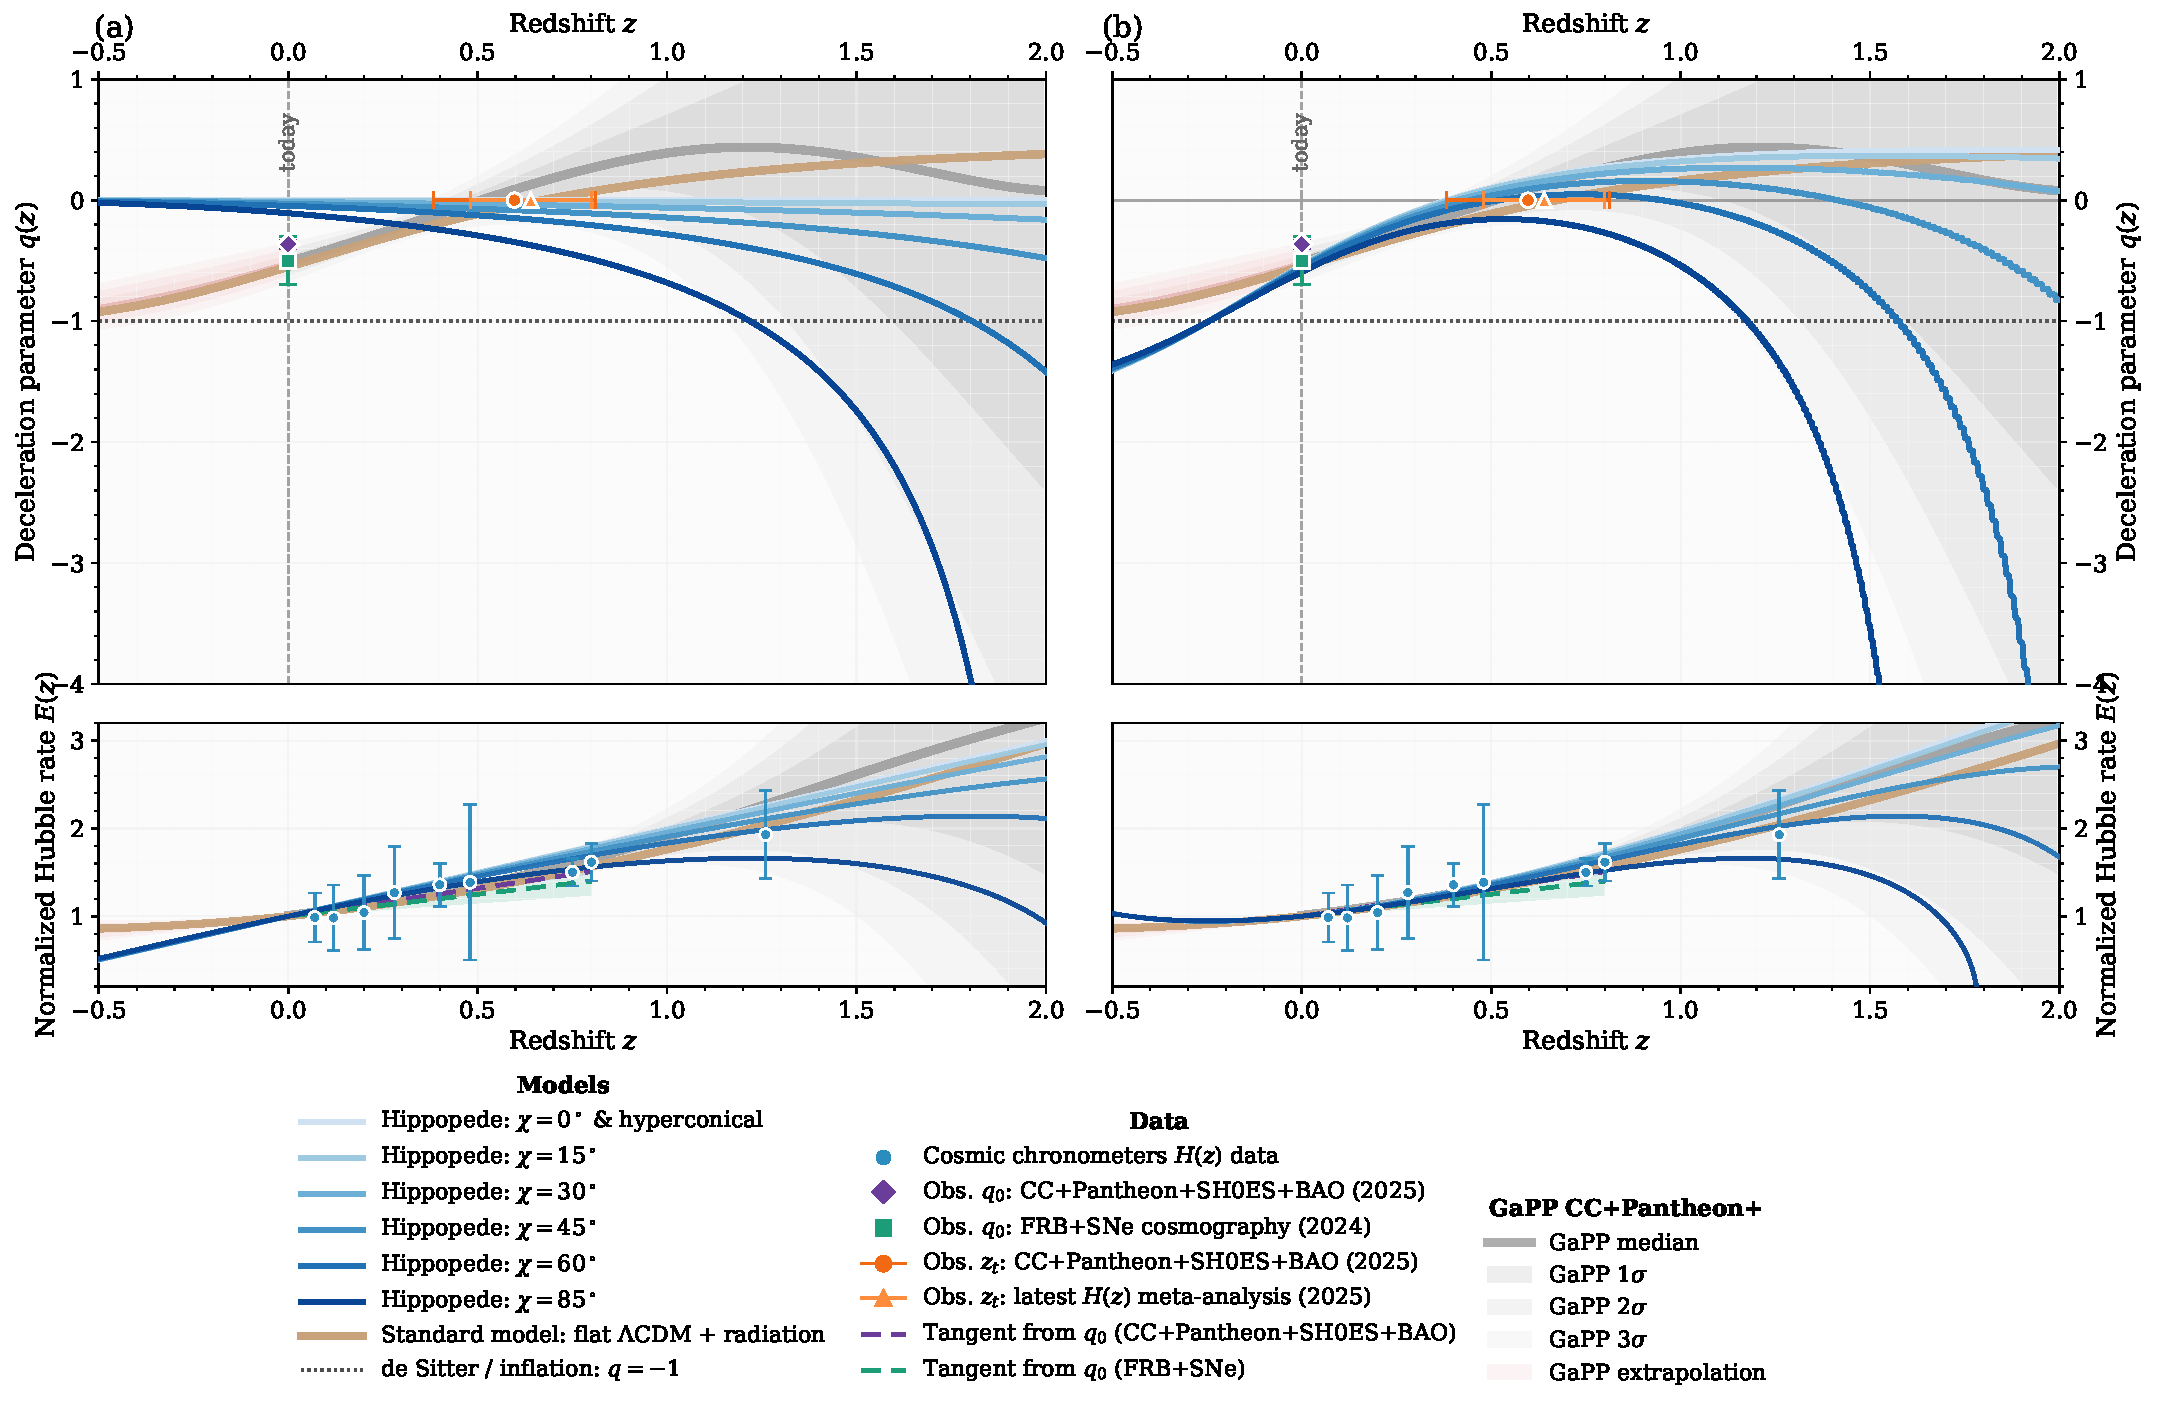
\includegraphics[width=\textwidth]{figures/hippopede_qz_centered_t0_3p0_double_panel_with_gapp}
\caption{
Comparison of the deceleration parameter $q(z)$ (top panels) and normalized expansion rate $E(z)=H(z)/H_0$ (bottom panels) for the centered-scale hippopede simulations (left block) and for the same centered histories after Monjo-type stereographic remapping (right block), both at fixed present time $t_0=3$. The colored curves correspond to the angular sectors $\chi=0^\circ,15^\circ,30^\circ,45^\circ,60^\circ,85^\circ$, while the thick light-brown curve shows the standard flat $\Lambda$CDM$+$radiation background. The upper panels include two present-day estimates of the deceleration parameter, $q_0=-0.364\pm0.032$ from CC+Pantheon+SH0ES+BAO and $q_0=-0.50\pm0.20$ from FRB+SNe cosmography, together with two transition-redshift determinations, $z_t=0.597\pm0.214$ and $z_t=0.64\pm0.16$ \cite{myrzakulov2025q0, gao2024frb, hu2025transition}. The lower panels include normalized cosmic-chronometer data and the GaPP reconstruction band obtained from CC+Pantheon$+$ data with the original Gaussian-process pipeline \cite{seikel2012gapp}. In the projected block the plotted value is $\alpha\simeq0.283$, following the preferred low-redshift implementation of \cite{monjo2018projected}; the Appendix explains why the same family also contains the asymptotic value $\alpha=1/2$ singled out by the radiation-like scaling requirement $H_{\mathrm{perc}}(T)\propto T^2$.}
\label{fig:qz_final}
\end{figure}

\subsection{Observational constraints on the projected model}

Applying the likelihood analysis described above to the DES-SN5YR supernova sample gives $\alpha_{\mathrm{eff}} = 0.323_{-0.012}^{+0.011}\;(1\sigma)$ with the result remaining stable across two independent \texttt{emcee} runs with different stretch-scale choices. Applying the same projected model to the DESI DR1 compressed BAO data gives $\alpha_{\mathrm{eff}} = 0.375_{-0.017}^{+0.016}\; (1\sigma)$, together with best-fit nuisance parameter $\beta = 28.85$ and $\chi^2_{\mathrm{best}}=12.39$ for 10 data points and 2 free parameters. For comparison, a flat $\Lambda$CDM fit with free $\Omega_m$ on the same BAO vector gives $\Omega_m = 0.289$ and $\chi^2_{\mathrm{best}}=11.72$, corresponding to $\Delta \mathrm{AIC}=0.68$. The two models are therefore statistically indistinguishable on the present DESI DR1 compressed BAO compilation.

\purple{Taken together, the supernova and BAO constraints probe distinct effective redshift ranges and remain consistent with a slow increase of the effective projection index relative to the low-redshift reference value $\alpha\simeq0.283$ discussed in \cite{monjo2018projected}.}

\begin{table}[h]
\centering
\color{purple}
\small
\caption{Summary of effective projected-hippopede constraints on $\alpha$.}
\label{tab:alpha_summary}
\begin{tabular}{lll}
\hline
Constraint & Redshift range & $\alpha_{\mathrm{eff}}$ \\
\hline
Low-$z$ projected reference \cite{monjo2018projected} & $z \rightarrow 0$ & 0.283 \\
DES-SN5YR \cite{abbott2024dark} & $0.025$--$1.3$ & $0.323_{-0.012}^{+0.011}$ \\
DESI DR1 BAO \cite{adame2025desi} & $0.295$--$1.491$ & $0.375_{-0.017}^{+0.016}$ \\
\hline
\end{tabular}
\end{table}



%The centered scale factor is defined on the $+u$ branch as $a_c^2=r^2+(u-t)^2$, and the corresponding directional redshift is given by $1+z_\chi=a_{c,\chi}(t_0)/a_{c,\chi}(t)$.

%The limit $\chi=0^\circ$ coincides with the hyperconical reference. The thick light-brown curve shows the standard flat $\Lambda$CDM background with radiation, while the dotted horizontal line marks the de Sitter reference $q=-1$.


At the same time, one should not overstate the analytical control of the projected model. The second-order analytic expansion used in the hyperconical literature is only a local approximation around $z=0$. In practice, the analytic approximation is useful only in a limited neighborhood of the present epoch; for the full displayed interval shown in the figure, the numerical prescription is the relevant one.

A second limitation concerns the interpretation of the projection parameter itself. The value $\alpha\simeq0.283$ gives the best low-redshift phenomenological agreement in the present implementation, but the projected family also contains the asymptotic value $\alpha=1/2$, which is selected by the high-redshift condition that the perceived thermal history satisfies $H_{\mathrm{perc}}(T)\propto T^2$. The two values need not be contradictory: the former can be understood as an effective late-time observational parameter, whereas the latter plays the role of a local/asymptotic physical limit in the sense discussed by Monjo and Campoamor-Stursberg \cite{monjo2020lagrangian, monjo2023hubble}.

\purple{At the purely geometric level, the same appendix also clarifies how the quartic hippopede can be read as a bilobulated deformation of the hyperconical picture, with axial branches that recover the hyperconical $3$-sphere limit and with a possible negative-curvature bilobulated extension described there as a separate geometric generalization rather than as part of the fitted late-time model.}

\blue{The same projected construction also suggests an effective observational isotropization toward high redshift. The anisotropy is clearly visible in the low-redshift dipole-like modulation, but the oblique sectors have a much shorter projected redshift reach than the nearly axial branch, so the observable window is expected to become progressively dominated by the preferred direction at sufficiently early apparent times. Since this point is directly relevant to the BBN-oriented interpretation, we discuss it in more detail in the Appendix.}

\subsubsection{\blue{Interpretation and limitations}}

Centered scale factor provides a cleaner phenomenological bridge between the quartic hypersurface and the asymptotic tangent-sphere picture than the origin-based scale factor. 

\blue{A separate numerical diagnostic indicates that the projected centered histories are indeed close to a dipole-like angular modulation over the low-redshift interval relevant to current background data. Fitting the projected $E(\chi,z)$ curves to the form $E_0(z)[1+D_1(z)\cos\chi]$ over the sectors $\chi=0^\circ$--$85^\circ$ yields $R^2\simeq0.98$--$0.99$ for $0.1\le z\le1$, with fitted amplitudes $D_1\simeq0.006$, $0.024$, $0.055$ and $0.231$ at $z=0.1$, $0.3$, $0.5$ and $1$, respectively. This does not yet constitute a fit to a sky dipole anomaly, because no mapping to an observed celestial direction has been imposed, but it does show that the anisotropy generated by the model is numerically very close to a true dipolar modulation over the late-time window where the observational comparison is performed.}

The present comparison remains exploratory. It is based on a selected set of chronometer and kinematic summary points, not on a full statistical fit, and it depends on a numerical pipeline that includes interpolation, differentiation, branch selection after the first minimum of $a_{c,\chi}(t)$, and, in the projected case, a specific implementation of the Monjo-type remapping. These limitations do not invalidate the qualitative comparison, but they do indicate that any stronger observational claim should be postponed to a dedicated fitting analysis.


\section{Discussion and conclusions}

The hippopede universe is not obtained from a constant-curvature hyperboloid but from a null quadratic relation in an auxiliary ambient (2,4)-spacetime as for an AdS${}_5$ manifold, and the quartic nature of the physical hypersurface arises because the embedding variables depend nonlinearly on the coordinates. In this sense the model should be viewed neither as a standard dS/AdS spacetime nor as a pure hyperconical cone, but rather as an intermediate toy geometry in which the ambient-space quadratic structure survives while the induced 4-dimensional hypersurface acquires a richer anisotropic dynamics.

To avoid a possible misunderstanding, one should emphasize that the toy universe is not identified with the full null hypersurface of the $(2,4)$ ambient space. The latter would be five-dimensional. What is physically relevant here is a four-dimensional submanifold satisfying both the null relation and the angular compatibility condition $u = \rho\cos\chi$, or equivalently the immersed image of the physical variables inside that null hypercone with $u$-axis constraint.

The cleanest way to compare the constructions is to separate three layers. First, the hippopede is recovered from a quartic constraint in Euclidean variables. Second, the toy universe lifts that quartic relation to a $t$-dependent hypersurface in $\mathbb{R}^{1,4}$ whose asymptotic radius is hyperconical-like. Third, after introducing auxiliary coordinates such as $p=(2t\cos\chi,\sin\chi, \vec{\rho}) \in \mathbb{R}^{2,4}$, the same quartic relation is rewritten by constraining the $u$-axis of the null quadratic condition $\|p\|_{\scriptscriptstyle{(2,4)}}^2=0$ in a $(2,4)$-signature ambient space, the same as for an AdS${}_5$ universe. The quartic character of our 4D hippopede universe is therefore not lost; it is encoded in the nonlinear way in which the physical coordinates enter the auxiliary null cone.

In this sense, the dS/AdS hyperboloids, their degenerate null-cone limits, and the hippopede null condition all belong to the same ambient-space family of quadratic loci, although they correspond to different geometric realizations. The relation among them is therefore one of shared embedding structure rather than dynamical equivalence. In fact, the same quartic relation defines a toy expanding geometry whose large-$t$ limit reproduces the linear law associated with hyperconical models, but whose subleading term produces an early-time regularization and a direction-dependent acceleration. The model is best understood as a controlled anisotropic toy universe: simple enough to admit closed analytic expressions, yet nontrivial enough to test how far one can deform exact hyperconical coasting while preserving its large-time behaviour.


%The geometric and cosmological lessons of the construction can be summarized in a compact way. Geometrically, the hippopede furnishes an explicit bridge between a classical quartic curve and the null quadratic constraints familiar from ambient-space relativity. Cosmologically, its four-dimensional extension shows that an asymptotically linear late expansion can coexist with a very different early-time acceleration pattern. 

\section*{\blue{Data Availability}}

\blue{The numerical scripts used to generate the figures are included in the project folder together with the local data files required for the final four-panel comparison figure. In particular, Fig.~\ref{fig:hippopede_growth_3d} is produced by \texttt{plot\_hippopede\_growth\_3d.py}, whereas Fig.~\ref{fig:qz_final} is produced by \texttt{plot\_hippopede\_qz\_double\_panel\_with\_gapp.py}. The supplementary diagnostic script \texttt{analyze\_hippopede\_dipole\_bbn.py} reproduces the late-time dipole-like fit and the constant-$\alpha$ BBN-oriented thermal checks reported in the main text and Appendix, while \texttt{analyze\_hippopede\_variable\_alpha.py} reproduces the running-$\alpha$ scans discussed in the Appendix. The dedicated thermal-history comparison against the standard radiation curve and the observationally inferred BBN corridor is generated by \texttt{plot\_hippopede\_projected\_thermal\_history\_bbn.py}. The bundled data directory contains the curated CC/BAO compilation, the local binned Pantheon$+$ input used by the GaPP reconstruction, and the local copy of the GaPP code needed to reproduce the figure.}

\bibliographystyle{unsrt}
\bibliography{main-hippopede}


\section*{Appendix}

\subsubsection*{Late-epoch linear expansion} 

The description of the hyppopede universe produces an anisotropic acceleration. If one now reads $t$ as a cosmic parameter for the origin-prescription approach and keeps the angular sector $\chi$ fixed, the directional scale factor of this toy model is
\begin{equation}
a_\chi(t):=\rho(t,\chi)=\sqrt{\sin^2\chi+4t^2\cos^2\chi}.
\end{equation}
In this origin-prescription focus, its directional Hubble, acceleration and deceleration functions are then
\begin{equation}
H_\chi(t)=\frac{\dot a_\chi}{a_\chi}=\frac{4t\cos^2\chi}{\sin^2\chi+4t^2\cos^2\chi},
\end{equation}
\begin{equation}
\ddot a_\chi(t)=\frac{4\cos^2\chi\,\sin^2\chi}{\left(\sin^2\chi+4t^2\cos^2\chi\right)^{3/2}},
\end{equation}
\begin{equation}
q_\chi(t):=-\frac{a_\chi\ddot a_\chi}{\dot a_\chi^2}=-\frac{\tan^2\chi}{4t^2}.
\end{equation}
Therefore the model is mildly accelerated for every oblique direction $0<|\chi|<\pi/2$, but the acceleration decays rapidly and
\begin{equation}
H_\chi(t)=\frac{1}{t}+O(t^{-3}),\qquad \ddot a_\chi(t)=\frac{\sin^2\chi}{2|{\cos\chi}|\,t^3}+O(t^{-5}),\qquad q_\chi(t)\to0^-.
\end{equation}
This is the precise sense in which the hippopede universe approaches linear expansion at late times: the asymptotic law is coasting, $a_\chi(t)\sim 2|{\cos\chi}|\,t$, even though the early epoch can display a nonzero positive acceleration. The limiting cases are also transparent: $\chi=0$ gives $a_0(t)=2t$ and hence exact linear expansion for all $t$, while $\chi=\pi/2$ gives $a_{\pi/2}(t)=1$, i.e. no expansion in the purely transverse direction. Numerically, for $\chi=\pi/4$ one finds $q_{\pi/4}(1)=-0.25$, $q_{\pi/4}(2)=-0.0625$, and $q_{\pi/4}(10)=-0.0025$, so the deviation from the linear regime dies off quickly.

\subsubsection*{Early-epoch accelerated universe}



The opposite limit is also informative. For any fixed oblique direction with $\sin\chi\neq0$,
\begin{equation}
a_\chi(0)=|\sin\chi|,\qquad \dot a_\chi(0)=0,\qquad \ddot a_\chi(0)=\frac{4\cos^2\chi}{|\sin\chi|}.
\end{equation}
Since $q_\chi(t)=-\tan^2\chi/(4t^2)$, the deceleration parameter is not merely large near $t=0$; it diverges to $-\infty$ for every fixed oblique direction with $\chi\neq0$. Numerically, for $\chi=\pi/6$ one finds $q_\chi(1)=-0.0833$, $q_\chi(0.5)=-0.333$, and $q_\chi(0.1)=-8.33$, while for $\chi=\pi/4$ the corresponding values are $-0.25$, $-1$, and $-25$. Thus the model becomes extremely accelerated at early times unless one approaches the privileged axis $\chi=0$. If one wishes to compare the toy model with observationally inferred $q(z)$, the next step would be to introduce an effective isotropized scale factor $a_{\mathrm{eff}}(t)$ and then use $1+z=a_{\mathrm{eff}}(t_0)/a_{\mathrm{eff}}(t)$ to map the directional dynamics into redshift space. A dedicated fit is therefore possible, but it requires an additional averaging prescription and should probably be presented separately as a numerical extension rather than as part of the conceptual derivation given here.
Hence the toy universe does not shrink to a point uniformly as $t\to0$: most angular sectors retain a finite initial radius and start with vanishing expansion rate but positive acceleration. The axis $\chi=0$ is singular in this limit, since $a_0(t)=2t$ collapses linearly to zero while the oblique sectors remain finite. This nonuniform behaviour is another sign that the model should be read as a biaxial toy geometry rather than as a realistic isotropic cosmology.


\subsubsection*{Bilobulated interpretation, axial hyperconical limit, and a possible $K=-1$ extension}

The large-$t$ geometry of the quartic model is best interpreted in two complementary ways. In the origin-based description one has
\begin{equation}
\rho(t,\chi)=\sqrt{\sin^2\chi+4t^2\cos^2\chi}
=2|{\cos\chi}|\,t+\frac{\sin^2\chi}{4|{\cos\chi}|\,t}+O(t^{-3}),
\end{equation}
so the leading term reproduces the dipolar law of the two tangent $3$-spheres discussed in the main text. Since the hyperconical universe of Monjo is foliated by spatial $3$-spheres of radius proportional to $t$, this is the precise sense in which each axial branch of the hippopede approaches a hyperconical branch at late times. Along the preferred directions $\chi\approx0$ and $\chi\approx\pi$, the quartic model therefore recovers the same linear coasting behaviour as the hyperconical construction, while the oblique sectors retain the anisotropic correction encoded in the subleading term.

The centered description clarifies the geometry of each individual lobe. On the $+u$ branch we defined
\begin{equation}
a_{c,\chi}(t):=\sqrt{r^2+(u-t)^2}
=\sqrt{\rho(t,\chi)^2+t^2-2t\,\rho(t,\chi)\cos\chi}.
\end{equation}
Using the same large-$t$ expansion for $\rho(t,\chi)$ one finds
\begin{equation}
a_{c,\chi}(t)^2
=t^2+\frac{\sin^2\chi}{2}+O(t^{-2}),
\qquad
a_{c,\chi}(t)
=t+\frac{\sin^2\chi}{4t}+O(t^{-3}).
\end{equation}
Thus, when each branch is viewed from the center of curvature of its own asymptotic tangent sphere, the lobe tends to a linearly expanding spatial $3$-sphere. This is again compatible with the hyperconical picture, because the constant-time spatial sections of the latter are themselves $3$-spheres. The difference is therefore mainly one of viewpoint: the origin-based picture emphasizes the dipolar two-branch structure, whereas the centered picture emphasizes the local recovery of a single hyperconical lobe.

This also shows why the bilobulated interpretation is close to, but not identical with, the quartic hippopede. The neck joining the two asymptotic lobes is certainly the most visible new geometric feature, but it is not the only one. Away from the strict large-$t$ limit the quartic relation leaves a residual angular deformation throughout the profile, and this is precisely what produces the anisotropic correction
\begin{equation}
\rho(t,\chi)-2|{\cos\chi}|\,t
=\frac{\sin^2\chi}{4|{\cos\chi}|\,t}+O(t^{-3}).
\end{equation}
In that sense, the hippopede should be viewed as a bilobulated hyperconical deformation: the neck expresses the global two-lobe topology, while the quartic angular term controls how the geometry departs from a pair of exact hyperconical branches at finite $t$.

The same intuition suggests a natural negative-curvature extension, although this goes beyond the exact quartic model studied in the main text. One may consider a compact hyperbolic $3$-manifold $N$ with totally geodesic boundary $\partial N\cong\Sigma_g$, where $\Sigma_g$ is a closed surface of genus $g\ge2$, and form the double
\begin{equation}
M_g=N\cup_{\phi}\bar N,
\end{equation}
with $\phi:\Sigma_g\to\Sigma_g$ an orientation-reversing boundary isometry. The resulting closed manifold carries a smooth metric of constant sectional curvature $K=-1$ and provides a mathematically natural bilobulated space with a geodesic neck. A cosmological line element of the form
\begin{equation}
ds^2=-dt^2+a(t)^2 h_{ij}dx^i dx^j,
\end{equation}
with $h_{ij}$ the hyperbolic metric on $M_g$, then defines a negatively curved FRW-type extension of the same bilobulated intuition.

However, this $K=-1$ construction should be interpreted carefully. The standard geodesic-polar expression
\begin{equation}
d\ell^2=d\rho^2+\sinh^2\rho\,d\Omega_2^2
\end{equation}
describes the simply connected space $H^3$ around a chosen point, not the full global geometry of a compact double $M_g$. Likewise, the quartic hippopede relation is not literally recovered as a global section of an arbitrary hyperbolic double. The connection is therefore structural rather than exact: the quartic model provides the explicit anisotropic toy geometry studied in this paper, whereas the doubled hyperbolic manifolds furnish a natural family of bilobulated negative-curvature analogues in which the neck is global and the asymptotic hyperconical intuition is replaced by hyperbolic ends or local axial neighbourhoods. The present work establishes the former rigorously and leaves the latter as a plausible geometric extension for future study.


\subsubsection*{Projected thermal asymptotics and the BBN-motivated limit $\alpha=1/2$}

To discuss primordial nucleosynthesis in the projected picture, one must distinguish between the intrinsic geometric time and the perceived thermal history of the projected radiation sector. The latter is the relevant quantity for BBN. Assuming the minimal adiabatic identification $T_{\mathrm{perc}}\propto 1+z$ (up to the usual slowly varying entropy factor $g_{*S}$), the high-redshift behaviour of the projected Hubble function follows directly from the asymptotics of the Monjo-type projection.

For $k=1$ one has $x_{\max}=\sqrt{3}/2$ and $b(x)=\sqrt{1-x^2}$, with $b(x_{\max})=1/2$. Writing $x=x_{\max}-\delta$ with $\delta\downarrow0$, one finds
\begin{equation}
2b-1\;=\;2\sqrt{1-x^2}-1\;=\;-2\sqrt{3}\,\delta+O(\delta^2),
\end{equation}
while
\begin{equation}
\sqrt{1-(1-b)^2}=\sqrt{2b-b^2}=\frac{\sqrt{3}}{2}+O(\delta).
\end{equation}
Therefore the line-of-sight integrand behaves as
\begin{equation}
\frac{\sqrt{1-(1-b)^2}}{b[2(b-1)+1]}
\;=\; -\frac{1}{2\delta}+O(1),
\end{equation}
so that
\begin{equation}
\xi_1(x)= -\frac12\ln\delta + O(1).
\end{equation}
Since $\xi_1(x)=\ln(1+z)$, this implies the boundary relation
\begin{equation}
\delta=x_{\max}-x(z)\propto (1+z)^{-2}.
\end{equation}

Now define $\eta:=\gamma_0-\gamma(x)$. Because $\gamma'(x)=1/\sqrt{1-x^2}$ is finite at $x=x_{\max}$, one has $\eta\propto\delta$. Near the boundary, the Monjo-type projection
\begin{equation}
f_{\hat r}^{\alpha}(x)=2\arctan\!\left[\frac{\gamma(x)/2}{(1-\gamma(x)/\gamma_U)^\alpha}\right]
\end{equation}
obeys
\begin{equation}
\frac{df_{\hat r}^{\alpha}}{dx}\propto \eta^{\alpha-1}\propto \delta^{\alpha-1}.
\end{equation}
Combining this with $dx/dz\propto (1+z)^{-3}$ gives
\begin{equation}
\frac{d\hat r}{dz}\propto (1+z)^{-(1+2\alpha)},
\qquad
\hat H(z)=\left(\frac{d\hat r}{dz}\right)^{-1}\propto (1+z)^{1+2\alpha}.
\end{equation}
Hence the projected family satisfies the asymptotic law
\begin{equation}
E_{\mathrm{hyp}}^{\mathrm{proj}}(z)\propto (1+z)^n,
\qquad n=1+2\alpha.
\end{equation}
Under the perceived thermal identification $T_{\mathrm{perc}}\propto 1+z$, this becomes
\begin{equation}
H_{\mathrm{perc}}(T)\propto T^{1+2\alpha}.
\end{equation}
The radiation-dominated standard law $H(T)\propto T^2$ is therefore recovered precisely when
\begin{equation}
\alpha=\frac12.
\end{equation}

\blue{The asymptotic exponent, however, is only part of the BBN requirement. A direct numerical calibration of the same projected prescription, performed with the extended lookup implemented in \texttt{analyze\_hippopede\_dipole\_bbn.py}, gives $n_{\mathrm{eff}}=1.999999$ over the interval $10^3\lesssim z\lesssim10^6$, as expected for $\alpha=1/2$, but the corresponding physical normalization obtained from $H_{\mathrm{perc}}(T)=H_0E_{\mathrm{hyp}}^{\mathrm{proj}}(T/T_0-1)$ is still too large by an approximately constant factor $H_{\mathrm{perc}}/H_{\mathrm{rad}}\simeq10.2$ in the representative BBN temperature range $T\simeq0.07$--$1\,\mathrm{MeV}$ when compared with the standard radiation-era law. Thus the constant-$\alpha$ branch with $\alpha=1/2$ reproduces the correct $T^2$ scaling but not yet the standard normalization.}

\blue{This observation motivates a second, more flexible numerical test within the same projected family: instead of identifying a single constant projection index, one may allow a smooth perceived-history interpolation}
\begin{equation}
\blue{
\alpha(z)=\alpha_{\mathrm{low}}+\frac{\alpha_{\mathrm{high}}-\alpha_{\mathrm{low}}}{2}
\left[
1+\tanh\!\left(
\frac{\ln(1+z)-\ln(1+z_c)}{2}
\right)
\right],
}
\end{equation}
\blue{with $\alpha_{\mathrm{low}}=0.283$ fixed by the successful low-redshift phenomenology of Fig.~\ref{fig:qz_final}, and $\alpha_{\mathrm{high}}=1/2$ fixed by the radiation-like asymptotic requirement. Exploratory scans with the supplementary script \texttt{analyze\_hippopede\_variable\_alpha.py}, checked directly against the literal projected-map relation $H_{\mathrm{perc}}(T)=H_0E_{\mathrm{hyp}}^{\mathrm{proj}}(T/T_0-1)$, show that the most promising BBN-like window is obtained for an earlier and narrower transition, approximately around}
\begin{equation}
\blue{
z_c\sim 1.6\times10^4
}
\end{equation}
\blue{This choice preserves the low-redshift sector almost unchanged, since $\alpha(1)\simeq0.28302$ and $\alpha(2)\simeq0.28303$, while driving the projected thermal history very close to the standard radiation-era normalization across the BBN window. In the updated diagnostic we compare it directly with the observationally inferred BBN corridor obtained from the 2024 primordial-abundance fit $\Delta N_{\mathrm{eff}}=-0.10\pm0.21$ of \cite{schoneberg2024bbn}. A representative near-optimal case is}
\begin{equation}
\blue{
z_c=1.616\times10^4
}
\end{equation}
\blue{for which the geometric-mean normalization with respect to the standard radiation curve over the interval $T\simeq0.07$--$1\,\mathrm{MeV}$ is}
\begin{equation}
\blue{
\left\langle \frac{H_{\mathrm{perc}}}{H_{\mathrm{rad}}}\right\rangle_{\mathrm{geom}}
\simeq 0.9915,
}
\end{equation}
\blue{with pointwise values}
\begin{equation}
\blue{
\frac{H_{\mathrm{perc}}}{H_{\mathrm{rad}}}\approx
0.991,\ 0.992,\ 0.993,\ 0.991,\ 0.991
}
\end{equation}
\blue{at $T=0.07,\ 0.10,\ 0.20,\ 0.50,\ 1.0\,\mathrm{MeV}$, respectively. Relative to the BBN-inferred central history of \cite{schoneberg2024bbn}, the corresponding residuals are only $-1.2\times10^{-3},\ 4.0\times10^{-4},\ 1.0\times10^{-3},\ -1.2\times10^{-3},\ -6.3\times10^{-4}$ over the same five temperatures. In the plotted diagnostic these values are read from the same literal projected-map evaluation after the mild log-space smoothing mentioned above, which removes small non-physical spikes produced by numerical differentiation of the dense lookup table without changing the BBN-window normalization in any material way. In other words, the same projected family admits a smooth perceived thermal history for which the whole BBN window is brought extremely close not only to the standard radiation background, but also to the currently inferred observational BBN corridor, rather than remaining strongly suppressed in the low-redshift constant-$\alpha$ branch or enhanced by more than one order of magnitude in the pure $\alpha=1/2$ branch.}

\blue{This does not yet amount to a full light-element calculation, and we therefore do not claim in this paper that the primordial abundances are already reproduced in detail. Nevertheless, the numerical result is strong enough to support a more focused statement: within the projected-hyperconical interpretation, the apparent thermal history can be made quantitatively compatible with both the normalization and the asymptotic $T^2$ scaling expected for a BBN-like radiation era, provided one allows a smooth transition from the low-redshift phenomenological value $\alpha\simeq0.283$ to the asymptotic physical value $\alpha=1/2$. A complete BBN claim would then require the next layer of analysis, namely a consistent treatment of $g_{*S}(T)$, the weak-interaction freeze-out, and the light-element reaction network.}

\blue{The same numerical exploration clarifies how the inherited anisotropy enters the projected early-time discussion. If one tries to construct a genuinely sector-dependent quantity}
\begin{equation}
\blue{
R_\chi(T):=\frac{H_{\chi,\mathrm{perc}}(T)}{H_{\mathrm{rad}}(T)},
}
\end{equation}
\blue{using the projected centered histories themselves, one finds that each fixed angle $\chi$ has only a finite internal redshift support. For the centered branches adopted in this work, the maximum unprojected redshifts are approximately}
\begin{equation}
\blue{
z^*_{\max}\simeq 3.0\times10^4,\ 12.36,\ 5.87,\ 3.78,\ 2.80,\ 2.13
}
\end{equation}
\blue{for $\chi=0^\circ$, $15^\circ$, $30^\circ$, $45^\circ$, $60^\circ$ and $85^\circ$, respectively. When these endpoints are translated back through the common projected-hyperconical map with $\alpha=1/2$, they correspond only to}
\begin{equation}
\blue{
z_{\mathrm{obs},\max}\simeq 422,\ 7.64,\ 5.01,\ 3.87,\ 3.23,\ 2.74,
}
\end{equation}
\blue{or, equivalently, to perceived temperatures of order}
\begin{equation}
\blue{
T_{\max}\simeq 9.9\times10^{-8},\ 2.0\times10^{-9},\ 1.4\times10^{-9},\ 1.1\times10^{-9},\ 1.0\times10^{-9},\ 8.8\times10^{-10}\ \mathrm{MeV}.
}
\end{equation}
\blue{These scales lie far below the standard BBN window $T\sim0.07$--$1\,\mathrm{MeV}$. Therefore the present centered branch does not yet provide a full anisotropic BBN calculation sector by sector: the oblique projected histories simply terminate long before one reaches the redshifts relevant to primordial nucleosynthesis.}

\blue{This is nevertheless physically informative. It means that the stereographic remapping does not erase the underlying anisotropy, but it does strongly filter its observational visibility. The oblique sectors dominate the low-redshift phenomenology and are responsible for the dipole-like modulation discussed in the main text, whereas at sufficiently high apparent redshift the observer progressively loses access to those sectors and is left mainly with the nearly axial branch. In that sense the projected model suggests an effective observational isotropization toward high redshift: the background remains intrinsically anisotropic, yet the observable radiation history becomes increasingly dominated by the preferred direction. The running-$\alpha$ BBN-like result obtained above should therefore be interpreted as an effective perceived thermal history of the projected radiation sector, not as a complete primordial-nucleosynthesis solution on the anisotropic centered background itself.}

\end{document}




===== REMOTE OVERLEAF VERSION =====
\documentclass[11pt]{article}

\usepackage{amsmath,amssymb,amsfonts}
\usepackage{xcolor}
\usepackage{authblk}
\usepackage{geometry}
\usepackage{graphicx}
\usepackage{hyperref}
\usepackage{chngcntr}
\geometry{margin=1in}
\graphicspath{{figures/}}
\DeclareGraphicsExtensions{.pdf,.png,.jpg}
\renewcommand{\vec}[1]{\boldsymbol{#1}}
\newcommand{\blue}[1]{{\color{blue}#1}}
\newcommand{\purple}[1]{\textcolor{purple}{#1}} 
\newcommand{\red}[1]{{\color{red}#1}}
\renewcommand\Authfont{\normalsize}
\renewcommand\Affilfont{\small}
\counterwithout{table}{section}
\renewcommand{\thetable}{\arabic{table}}

\title{Hippopede Universe as a toy model of late-linear expansion}
\author[1,2]{Robert Monjo}
\author[3]{Manel Romero}
\author[4]{Ardra E. Sasi}
\affil[1]{Department of Mathematics, CUNEF University, Calle Almansa 101, Madrid 28040, Spain}
\affil[2]{Centro de Estudios Cosmologicos ``Prof. Jaime Roessler Bonzi'', Facultad de Ciencias, Universidad de Chile, Las Palmeras 3425, \~Nunoa, Santiago 7750000, Chile}
\affil[3]{Area of Chemistry, University of Barcelona, Campus Diagonal: Av. Joan XXIII, 27-31, 08028 Barcelona, Spain}
\affil[4]{School of Pure and Applied Physics
Mahatma Gandhi University, Priyadarsini Hills P.O. Athirampuzha, Kottayam, Kerala 686560, India}
\date{}

\begin{document}

\maketitle

\begin{abstract}

The hippopede is a classical quartic curve with a long history in geometry, yet it also offers a suggestive reinterpretation in modern embedding approaches. In this work we show that its defining relation can be recast as a null quadratic constraint in an auxiliary pseudo-Euclidean space, thereby placing the extended hippopede hypersurface in direct analogy with the ambient-space constructions commonly used for de Sitter and anti de Sitter geometries. We then apply the same quartic structure to a four-dimensional toy universe whose large-$t$ limit consists of two tangent $3$-spheres, so that the model becomes a simple laboratory for asking whether a hyperconical late-time coasting law can emerge together with a distinct early-time acceleration.

\end{abstract}

\section{Introduction}

\subsection{Motivation}

Model-dependent probes such as BAO and CMB fits, and more direct determinations based on cosmic chronometers (CC) and Type Ia supernovae (SNe Ia), do not always favour the same late-time expansion history. This discrepancy is visible both in the local Hubble tension and in the broader discussion of how background expansion should be inferred from intrinsic versus projection-dependent observables. In hyperconical approaches this distinction is especially relevant, because an apparently accelerated phenomenology can arise from the projection map even when the underlying ambient-space expansion remains asymptotically linear \cite{monjo2018projected, monjo2023hubble}.

A natural starting point for the present work is the long-standing interest in coasting cosmologies, namely models for which the late-time scale factor behaves approximately as $a(t)\propto t$. Such scenarios were studied early on by John et al. \cite{john2000coasting, John2019} as viable alternatives to standard decelerating or accelerated backgrounds, and more recently they have reappeared in hyperconical modified-gravity constructions where the linear law is tied to an ambient-space geometric constraint \cite{monjo2017hyperconical, Monjo_2024, Monjo_2025}. Within that framework, recent astrophysical tests indicate that the model can remain phenomenologically competitive beyond galactic rotation curves: hydrostatic-equilibrium analyses of X-COP clusters show good agreement in hot-gas-dominated regions beyond $\sim1\,\mathrm{Mpc}$, while galaxy--galaxy weak-lensing reconstructions yield flat circular velocities on megaparsec scales that compare favorably with MOND in the same regime \cite{monjo2025clusters, monjo2025lensing}.

The main cosmological motivation for relaxing exact coasting at all epochs comes from primordial nucleosynthesis. In a strictly linear expansion, $H(t)=1/t$, the Universe remains older at a fixed temperature than in the standard radiation-dominated scenario, so weak interactions stay effective for longer and the neutron-to-proton ratio freezes out under different conditions. This alters the synthesis window for light nuclei: in particular, it tends to overproduce helium and strongly affects deuterium survival unless additional assumptions are introduced \cite{sethi1999coasting, dev2002coasting}. For that reason, even if a late coasting regime is phenomenologically attractive, one is naturally led to explore toy geometries in which the large-$t$ behaviour remains asymptotically linear while the early-time acceleration differs from zero. The hippopede universe proposed below is meant precisely in that spirit: it is not offered as a realistic cosmology, but as a controllable biaxial toy model interpolating between a regular quartic geometry and a hyperconical-like late regime.

\subsection{Hippopede curve}
Algebraic curves of low degree have long played a role not only in classical geometry but also in astronomical modelling and, more recently, in modern theoretical physics. Among these curves, the \emph{hippopede} occupies a historically interesting position. The curve was already known in Greek geometry and is traditionally associated with the work of Eudoxus and later commentators such as Proclus, appearing in discussions of planetary motion and spherical constructions \cite{Gregory_2011, Taub2020, BotteriCasazza2023}. In modern mathematical terminology, the hippopede is a quartic plane curve that can be written in implicit form as the set of points $(x,y) \in \mathbb{R}^2$ satisfying:
\begin{equation}
    k x^2 + y^2 - (x^2+y^2)^2 = 0
\end{equation}
where $(x,y)$ are the Cartesian coordinates and $k > 0$ is a positive real constant.


The geometry of this curve and related quartic curves has been discussed in classical works on plane algebraic curves and in modern mathematical treatments of special curves. Standard references include the classical monograph of Lawrence \cite{lawrence1972catalogue} and more recent surveys of plane quartics such as those by Gibson \cite{gibson2001elementary}. From the viewpoint of differential geometry, the curve can also be viewed as a deformation of the circle controlled by the parameter $k$. Writing $k=4t^2$ and introducing polar coordinates $(r,\theta)$ defined by $x=r\cos\theta$ and $y=r\sin\theta$, the defining equation becomes $r^2 = 4t^2\cos^2\theta + \sin^2\theta$. This representation shows that the curve can be regarded as a deformation of the circle in which the radial coordinate depends on the polar angle. When $t=\tfrac12$ (equivalently $k=1$) the curve reduces to the unit circle. For $t >\tfrac12$ the curve develops the characteristic shape of the hippopede, elongated along the horizontal axis.

From the algebraic viewpoint the curve is a quartic plane curve symmetric under reflections across both coordinate axes. Its intersection with the coordinate axes is easily determined: the curve passes through $(0,\pm1)$ independently of the value of $k$, while its intersection with the horizontal axis occurs at $(\pm 2t,0)$. These properties make the hippopede a particularly simple example of a quartic curve whose geometry is controlled by a single parameter.

\subsection{Hyperconical, \textit{de Sitter} and \textit{anti de Sitter} geometries}

The hyperconical universe $\mathcal{H}^4$ is mathematically defined as the null hypersurface embedded in a pseudo-Euclidean manifold (flat ambient space) of signature $s=(1,4)$ or $s=(4,1)$, which is usually referred to as 5-dimensional Minkowskian spacetime $\mathbb{R}^s$ \cite{monjo2017hyperconical, Monjo_2024}. For instance, the $(4,1)$ convention can be written as follows:
\begin{equation}
\mathcal{H}^4:=\left\{q=(t,\vec{\rho})\in\mathbb{R}^{4,1}\;:\;-t^2+\|\vec{\rho}\|_{\scriptscriptstyle{(4,0)}}^2=0\right\},
\end{equation}where $\|\vec{\rho}\|_{\scriptscriptstyle{(4,0)}} ^2$ represents the quadratic form of $\vec{\rho} = (x,y,z,u)$ in $\mathbb{R}^4$, that is, $\|\vec{\rho}\|_{\scriptscriptstyle{(4,0)}} ^2 = x^2+y^2+z^2+u^2$. Equivalently, on each constant-$t$ slice one has $\|\vec{\rho}\|_{\scriptscriptstyle{(4,0)}} =t$, so the spatial section is a 3-sphere of radius $t$ and the resulting background expands linearly. By contrast, the 4-dimensional de Sitter (dS${}_4$) spacetime is described by the hyperboloid $-X_0^2+X_1^2+X_2^2+X_3^2+X_4^2=\alpha^2$ in the same ambient-space $\mathbb{R}^{4,1} \ni (X_0, \dots X_4) = X$, but with nonzero curvature radius $\alpha = \|X\|_{\scriptscriptstyle{(4,1)}}$. Within this embedding picture, the hyperconical universe may be regarded as the degenerate limit $\alpha\to0$ of the dS${}_4$ family, for which the regular hyperboloid collapses to the null cone. It is therefore better described as a singular limit of dS geometry than as an ordinary dS spacetime. 

Finally, a $4$-dimensional \textit{anti de Sitter} (AdS${}_4$) spacetime is a pseudo-Riemannian manifold embedded by increasing up to two time coordinates $(t_1, t_2)$, which satisfy $-t_1^2-t_2^2+X_1^2+X_2^2+X_3^2 = - \alpha$ in a pseudo-Euclidean space $\mathbb{R}^{3,2}$ with signature $(3,2)$.  Thse constructions provide a powerful geometric representation of constant curvature cosmological spacetimes and is standard in the literature on relativistic cosmology and quantum field theory in curved spacetime \cite{hawking1973large, spradlin2001les}.

What these constructions share is the quadratic embedding language, and this is exactly the bridge on which the present toy model is built. The hippopede extension sits between both pictures: like the hyperconical case, it has an asymptotically linear radius; like the dS/AdS constructions, it is most naturally understood through a higher-dimensional quadratic relation. Hyperconical models have been proposed precisely because they realize a linear late expansion law in a natural embedding setting \cite{monjo2017hyperconical}. It is therefore natural to ask whether nearby toy models can preserve the asymptotic coasting behaviour $a(t)\propto t$ while allowing a different acceleration pattern during early epochs. The higher--dimensional hippopede provides a minimal laboratory for that question: it keeps the same large-$t$ linear scaling along the expanding directions, but it regularizes the exact hyperconical behaviour by a finite angular term that modifies the early dynamics.


The logic of the paper is therefore fourfold: first, we identify the correct high--dimensional extension of the quartic relation; second, we extract its large-$t$ limit as two tangent hyperspheres, with the intention of a hyperconical toy universe; third, we compute the corresponding directional Hubble and acceleration functions; and fourth, we relate the resulting quartic toy model to the ambient-space construction used for dS/AdS geometries.


\section{Data and Methods}

\subsection{Data}

We used observed estimates of the deceleration parameter collected from: i) the present deceleration estimates $q_0=-0.364\pm0.032$ together with the transition redshift estimate $z_t=0.597\pm0.214$ from the combined CC+Pantheon+SH0ES+BAO analysis \cite{myrzakulov2025q0}; ii) the cosmographic estimate $q_0=-0.50\pm0.20$ obtained from fast radio bursts (FRB) combined with supernovae (SNe) in \cite{gao2024frb}; iii) the screened meta-analytic transition estimate $z_t=0.64\pm0.16$ from the latest $H(z)$ compilation analysis of \cite{hu2025transition}. Moreover, observed estimates of normalized Hubble factor $E_{\mathrm{obs}}(z)=H(z)/H_0$ were computed from the CC measurements, with $H_0=70~\mathrm{km\,s^{-1}\,Mpc^{-1}}$ (Table \ref{tab:cc_data_figures}).

For the dedicated low-to-intermediate redshift constraints on the projected model, we additionally use two complementary datasets. The DES-SN5YR Type Ia supernova sample \cite{abbott2024dark} contains 1829 supernovae over the interval $0.025 \le z \le 1.3$. The compressed DESI DR1 baryon acoustic oscillation catalogue \cite{adame2025desi} provides measurements of $D_M/r_s$, $D_H/r_s$, and $D_V/r_s$ in six galaxy and quasar tracer bins centered at $z_{\rm eff}=0.295$, $0.510$, $0.706$, $0.930$, $1.317$, and $1.491$. In this first geometric analysis we exclude the Ly$\alpha$ forest point near $z_{\rm eff}\simeq2.33$, so that the fit remains restricted to the lower-redshift window most directly comparable with the supernova sector.

\begin{table}[h]
\centering
\small
\caption{Observational inputs used in this work.}
\label{tab:dataset_summary}
\begin{tabular}{lll}
\hline
Dataset & Observable(s) & Redshift range  \\
\hline
Cosmographic constraint \cite{myrzakulov2025q0,gao2024frb,hu2025transition} & $q_0$, $z_t$ & local to intermediate \\
Cosmic chronometers & $H(z)$, hence $E(z)=H/H_0$ & $0.07$--$1.26$ \\
CC+Pantheon$+$ GaPP \cite{seikel2012gapp} & reconstructed $q(z)$ and $E(z)$ & low to intermediate \\
*DES-SN5YR \cite{abbott2024dark} & SN distance moduli & $0.025$--$1.3$  \\
*DESI DR1 BAO \cite{adame2025desi} & $D_M/r_s$, $D_H/r_s$, $D_V/r_s$ & $0.295$--$1.491$ \\
\hline
\end{tabular}
\end{table}

Note:  *Likelihood constraint on $\alpha_{\mathrm{eff}}$

\begin{table}[h]
\label{tab:cc_data_figures}
\centering
\small

\caption{Observed values of the Hubble parameter according to the cosmic chronometers considered.}

\begin{tabular}{lll}
\hline
$z$ & $H(z)$ [km s$^{-1}$ Mpc$^{-1}$] & Source \\
\hline
0.07, 0.12, 0.20, 0.28 & 69.0$\pm$19.6,\;68.6$\pm$26.2,\;72.9$\pm$29.6,\;88.8$\pm$36.6 & Zhang et al. \cite{zhang2014hubble} \\
0.40, 0.48 & 95.0$\pm$17.0,\;97.0$\pm$62.0 & Stern et al. \cite{stern2010chronometers} \\
0.75 & 105.0$\pm$7.9(stat)$\pm$7.3(sys) & Jimenez et al. \cite{jimenez2023photometry} \\
0.80 & 113.1$\pm$15.1(stat)$^{+29.1}_{-11.3}$(sys) & Jiao et al. \cite{jiao2023legac} \\
1.26 & 135.0$\pm$35.0 & Tomasetti et al. \cite{tomasetti2023vandels} \\
\hline
\end{tabular}


\end{table}

Finally, Gaussian-process reconstructions obtained with the original GaPP logic are included in order to compare the centered hippopede histories with model-independent reconstructions of both $q(z)$ and $E(z)$ based on CC+Pantheon$+$ data \cite{seikel2012gapp}.



\subsection{Model}

\subsubsection{The coasting hippopede universe}

Let $(t, \vec \rho) = (t,x,y,z,u)\in\mathbb{R}^{1,4}$, and consider the hypersurface
\begin{equation}
\label{eq:hippopede_univ}
 x^2 + y^2 + z^2 + 4t^2 u^2 = (x^2 + y^2 + z^2 + u^2)^2 .
\end{equation}
defined as an upper-dimensional extension of the hippopede curve.

 Let $\rho^2 := \|\vec \rho\|_{\scriptscriptstyle{(4,0)}}^2$ with $\|\vec \rho\|_{\scriptscriptstyle{(4,0)}}^2=x^2 + y^2+z^2 + u^2 =: r^2 + u^2$ and introduce spherical coordinates around the distinguished $u$-axis,
\begin{equation}\label{eq:angle-constraint}
u=\rho\cos\chi,\qquad r=\rho\sin\chi.
\end{equation}
Then Eq.~\eqref{eq:hippopede_univ} becomes
\begin{equation}
\label{eq:hippopede_univ2}
\rho^2=\sin^2\chi+4t^2\cos^2\chi.
\end{equation}
Introducing the auxiliary coordinates
$t_1:=2t\cos\chi,\; t_2:=\sin\chi$,
the same relation is exactly equivalent to the null condition $\vec{\rho}^2-t_1^2-t_2^2=0$,
in a 6D ambient space with pseudo-Euclidean metric of signature $(2,4)$ or $(4,2)$. According to Eq. \ref{eq:angle-constraint}, the 4D hippopede hypersurface is therefore given by the dipolar-angle constraint $u^2-{\vec \rho}^2(1-t_2^2) = 0$ of the 6D null hypercone in the ambient space, where $u$ is the fourth coordinate of $\vec \rho$. This is the minimal consistent immersion formulation of the toy model, which is equivalent to encode the quartic hypersurface through a nonlinear map from the physical variables $(t,\chi)$ into an auxiliary null cone (Eq. \ref{eq:hippopede_univ2}). This exact expression already displays two key points: i) it contrasts with the \textit{light cone} $\{p = (t,\vec{\rho}) \in \mathbb{R}^{1,4}\;:\; \|p\|^2 = 0\}$ defined in the $(1,4)$-signature hyperconical universe; ii) along every direction with $\cos\chi\neq0$, the size of the configuration grows linearly with $t$ for large times, as in the $\mathbb{R}^{1,4}$ case. More precisely,
\begin{equation}
\rho(t,\chi)=2|{\cos\chi}|\,t+\frac{\sin^2\chi}{4|{\cos\chi}|\,t}+O(t^{-3})\qquad (t\to\infty).
\end{equation}
The leading term
\begin{equation}
\rho_{\infty}(t,\chi)=2|{\cos\chi}|\,t
\end{equation}
is exactly the dipolar equation of the union of the two tangent $3$-spheres
\begin{equation}
x^2+y^2+z^2+(u-t)^2=t^2,\qquad x^2+y^2+z^2+(u+t)^2=t^2.
\end{equation}
Indeed, each sphere of radius $t$ centered at $u=\pm t$ satisfies $\rho=2t|\cos\chi|$. In this sense the quartic hypersurface interpolates between a smooth finite-$t$ geometry and a double-sphere large-$t$ limit, which is the natural place to import the hyperconical-universe intuition into the hippopede setting.

At the purely geometric level, the most immediate ``origin-based'' reading of the quartic hypersurface is simply $a_{\chi}(t):=\rho(t,\chi)$.  If one now reads $t$ as a cosmic parameter and keeps the angular sector $\chi$ fixed, the directional scale factor of this toy model is
\begin{equation}
a_\chi(t):=\rho(t,\chi)=\sqrt{\sin^2\chi+4t^2\cos^2\chi}.
\end{equation}
Its directional Hubble $H_\chi(t)= \dot a_\chi / a_\chi$ and acceleration $\ddot a_\chi(t)$ determine its deceleration function as $q_\chi(t):= - a_\chi\ddot a_\chi / \dot a_\chi^2 = - a_\chi a_\chi\ddot / H_\chi(t)^2$. We remark on that prescription because it yields closed analytic expressions and provides a useful first contrast with the hyperconical case with pure linear expansion (see Appendix). However, the numerical results eventually adopted for the two definitive comparison figures are based instead on a centered effective scale factor measured with respect to the center of curvature of one asymptotic tangent branch.

\begin{figure}[t]
\centering

\includegraphics[width=0.78\textwidth]{hippopede_growth_3d}
\caption{Three-dimensional visualization of the nested hippopede hypersurfaces associated with increasing values (0.5, 1, 2 and 3.0) of the parameter $t$. The distinguished axis is $u$, while the orthogonal directions are represented through $(\sqrt{x^2+y^2},z)$. As $t$ grows, the quartic hypersurface approaches the large-time limit formed by two tangent 3-spheres centered at $u=\pm t$, making explicit the emergence of an asymptotically hyperconical coasting regime.}
\label{fig:hippopede_growth_3d}
\end{figure}


\subsection{\blue{Centered prescription}}

\blue{The analytic scale factor $a_\chi(t)=\rho(t,\chi)$ introduced above is the most direct reading of the quartic hypersurface, but the large-$t$ tangent-sphere limit also suggests a second effective radius measured from the center of curvature of one asymptotic branch. In the numerical figures we therefore define, on the $+u$ branch, the centered effective scale factor}
\begin{equation}
\blue{
a_{c,\chi}(t):=\sqrt{r^2+(u-t)^2}
=\sqrt{\rho(t,\chi)^2+t^2-2t\,\rho(t,\chi)\cos\chi}.
}
\end{equation}
\blue{This prescription is not meant to replace the intrinsic quartic relation; it is introduced only as a figure-level effective radius motivated by the double-sphere asymptotic geometry. The corresponding centered redshift, Hubble and deceleration functions used in the simulations are}
\begin{equation}
\blue{
1+z_\chi(t)=\frac{a_{c,\chi}(t_0)}{a_{c,\chi}(t)},\qquad
H_{c,\chi}(t)=\frac{\dot a_{c,\chi}(t)}{a_{c,\chi}(t)},\qquad
E_\chi(z)=\frac{H_{c,\chi}(t)}{H_{c,\chi}(t_0)},
}
\end{equation}
\begin{equation}
\blue{
q_\chi(z)=-\frac{a_{c,\chi}(t)\,\ddot a_{c,\chi}(t)}{\dot a_{c,\chi}(t)^2},
}
\end{equation}
\blue{with the derivatives evaluated numerically along each centered history. In the final comparison figures we fix $t_0=3$ and show the angular sectors $\chi=0^\circ,15^\circ,30^\circ,45^\circ,60^\circ,85^\circ$. The case $\chi=0^\circ$ is then identical to the unprojected hyperconical/coasting reference of the same centered prescription.}

\subsection{\blue{Projected prescription}}

\blue{To generate the projected simulations, we keep the same centered histories but remap them through the projected-hyperconical construction used by Monjo in the inhomogeneous hyperconical programme \cite{monjo2017hyperconical, monjo2018projected, monjo2020lagrangian, monjo2023hubble, Monjo_2024}. In the notation of \cite{monjo2018projected}, let}
\begin{equation}
\blue{
\xi_1(x):=\int_{0}^{x}\frac{\sqrt{1-(1-b)^2}}{b\left[2(b-1)+1\right]}\,d\tilde x,
\qquad
b=b(\tilde x):=\sqrt{1-\tilde x^2},
}
\end{equation}
\blue{be the dimensionless line-of-sight function of the $k=1$ hyperconical model, and define}
\begin{equation}
\blue{
x(z):=\xi_1^{-1}(\ln(1+z)).
}
\end{equation}
\blue{The preferred $\gamma$-projection is then written as}
\begin{equation}
\label{eq:projection_map}
\blue{
f_{\hat r}^{\alpha}(x):=
2\arctan\!\left[
\frac{\gamma(x)/2}{\left(1-\gamma(x)/\gamma_U\right)^\alpha}
\right],
}
\end{equation}
\blue{where}
\begin{equation}
\blue{
\gamma(x):=\arctan\!\left(\frac{x}{\sqrt{1-x^2}}\right)
,
\qquad \gamma_U:=\gamma(x_{\max}).
}
\end{equation}
\blue{For the $k=1$ hyperconical domain one has $x_{\max}=\sqrt{3}/2$, hence}
\begin{equation}
\blue{
\gamma_U=\arctan\!\left(\frac{\sqrt{3}/2}{1/2}\right)=\arctan(\sqrt{3})=\frac{\pi}{3}.
}
\end{equation}
\blue{The projected hyperconical proper distance is therefore}
\begin{equation}
\blue{
\hat r(z)= f_{\hat r}^{\alpha}\!\left(x(z)\right)
= f_{\hat r}^{\alpha}\!\left(\xi_1^{-1}(\ln(1+z))\right),
}
\end{equation}
\blue{and the associated projected reference Hubble function is defined by}
\begin{equation}
\blue{
\hat H(z):=\left(\frac{d\hat r}{dz}\right)^{-1},
\qquad
E_{\mathrm{hyp}}^{\mathrm{proj}}(z)=\frac{\hat H(z)}{\hat H(0)}.
}
\end{equation}
\blue{Each centered hippopede simulation is then projected through the common redshift remapping}
\begin{equation}
\blue{
z^*=E_{\mathrm{hyp}}^{\mathrm{proj}}(z)-1,
\qquad
E^{\mathrm{proj}}_\chi(z)=E_\chi(z^*),
}
\end{equation}
\begin{equation}
\blue{
q^{\mathrm{proj}}_\chi(z)=-1+(1+z)\frac{d\ln E^{\mathrm{proj}}_\chi(z)}{dz}.
}
\end{equation}
\blue{In the low-redshift phenomenological implementation used for Fig.~\ref{fig:qz_final}, we adopt the preferred observationally calibrated value $\alpha\simeq0.283$ discussed in \cite{monjo2018projected}. However, the local projected-hyperconical analysis of Monjo and Campoamor-Stursberg motivates a distinct asymptotic value, $\alpha=1/2$, when one asks for the projected early-time scaling to behave like a standard radiation-dominated thermal history \cite{monjo2020lagrangian, monjo2023hubble}. The two values should therefore be read as characterizing two different regimes of the same projected family: $\alpha\simeq0.283$ as an effective low-redshift phenomenological value, and $\alpha=1/2$ as the physically motivated asymptotic limit singled out by the high-redshift thermal argument developed below.}

\blue{If the projected redshift is interpreted as the perceived redshift of the radiation sector, a minimal adiabatic prescription gives}
\begin{equation}
\blue{
g_{*S}(T_{\mathrm{perc}})\,T_{\mathrm{perc}}^3 a_{\mathrm{perc}}^3=
\mathrm{const},
\qquad
T_{\mathrm{perc}}(z)\simeq T_0(1+z)
\left(\frac{g_{*S}(T_0)}{g_{*S}(T_{\mathrm{perc}})}\right)^{1/3}.
}
\end{equation}
\blue{Neglecting for the moment the slow variation of $g_{*S}$, one may simply write $T_{\mathrm{perc}}\propto 1+z$ and hence}
\begin{equation}
\blue{
H_{\mathrm{perc}}(T)=H_0 E_{\mathrm{hyp}}^{\mathrm{proj}}\!\left(\frac{T}{T_0}-1\right).
}
\end{equation}
\blue{This is the quantity relevant to the primordial-nucleosynthesis discussion, because BBN constrains the thermal relation $H(T)$ rather than the late-time deceleration function alone. In the Appendix we show that the Monjo-type family implies the asymptotic scaling $E_{\mathrm{hyp}}^{\mathrm{proj}}(z)\propto (1+z)^{1+2\alpha}$, so that the special value $\alpha=1/2$ yields the radiation-like law $H_{\mathrm{perc}}(T)\propto T^2$.}

\blue{The numerical implementation was carried out in Python (see scripts in the Data Availability statement). For the centered histories, derivatives were evaluated numerically on dense $t$-grids and the branch after the first minimum of $a_{c,\chi}(t)$ was retained whenever needed to avoid multivalued redshift histories. For the projected case, the Monjo-type redshift map was implemented numerically from the preferred $\mathrm{inv.ll}$ prescription and then used as a common remapping of the centered simulations. This should be kept in mind when interpreting the projected curves: they are numerically stable over the displayed interval, but they still depend on the chosen projection prescription and on the numerical differentiation/interpolation strategy. In the dedicated thermal-history diagnostic, the running-$\alpha$ branch is displayed after a very mild moving-average smoothing in $\log H$, introduced only to suppress small derivative artefacts generated by the dense boundary lookup of the literal projected map; the quoted BBN-window ratios change only at the percent level under this cosmetic filtering. The comparison corridor shown in that diagnostic is no longer a purely heuristic $\Delta N_{\mathrm{eff}}$ band, but an observationally inferred one based on the 2024 primordial-abundance analysis of \cite{schoneberg2024bbn}. The anchor points shown on that diagnostic are therefore not direct measurements of $H(T)$, but representative BBN-inferred sampling points placed on the central inferred expansion curve of \cite{schoneberg2024bbn}; correspondingly, the lower panel is plotted in terms of residuals with respect to that inferred central history, so that the main competition between the standard radiation branch and the projected hyperconical branch is visually explicit. For comparison we also plot a flat $\Lambda$CDM$+$radiation background with $\Omega_r=9\times10^{-5}$, $\Omega_m=0.3$, and $\Omega_\Lambda=0.69991$.}

\subsection{\purple{Likelihood analysis for the projected model}}

\purple{The normalized expansion rate $E(z)$ of the geometric projection is then used to define the angular diameter distance
\begin{equation}
    D_A(z) = \frac{1}{1 + z} \int_{0}^{z} \frac{dz'}{E^{\mathrm{proj}}(z')}
\end{equation}
Here $D_A$ is dimensionless and the overall $c/H_0$ is absorbed by the nuisance parameters analytically eliminated in each likelihood. The central quantity of interest is the parameter $\alpha$, as it controls the degree of stereographic distortion in mapping from the hyperconical geometry to the observable distance-redshift relation. In the isotropic limit $(\chi = 0^\circ)$, $\alpha$ is the single free parameter of the model. Rather than a strict constant, $\alpha$ is predicted to run slowly with redshift \cite{monjo2018projected}, increasing from $\alpha \approx 0.283$ at $z \rightarrow 0$ toward higher values at intermediate and high redshifts. When a single constant $\alpha$ is fitted over a finite redshift window, the recovered value reflects the effective mean of $\alpha(z)$ over that window.}

\purple{In both analyses the likelihood is kept purely geometric, with nuisance parameters eliminated analytically rather than sampled. For the supernova analysis, the absolute magnitude $M_B$ - fully degenerate with $H_0$ - is analytically marginalized. For the BAO analysis, the sound horizon $r_s$ is not independently defined within the projected hyperconical framework, since the model describes only late-time expansion history and does not commit to the early-universe physics that sets $r_s$. The combined nuisance $\beta = c/(H_0r_s)$ is therefore marginalized in the same spirit. This avoids importing $\Lambda$CDM assumptions for the pre-recombination era. This places both analyses on equal footing --- each reduces to fitting the shape of $E(z)$ with $\alpha$ as the single parameter and one analytically eliminated nuisance.}

\purple{For a given $\alpha$, the expansion rate $E(z)$ is computed on a dense internal grid, with the derivative $d\hat{r}/dz$ evaluated by finite differences on this uniform grid to ensure numerical stability.}

\purple{For the supernova analysis, dimensionless angular diameter distance is evaluated in a CosmoSIS plugin integrated with the Dovekie likelihood code, which then compares the model distance modulus}
\begin{equation}
    \purple{\mu(z) = 5\log_{10}[(1 + z_{CMB})(1 + z_{HEL})D_A(z)] + 25}
\end{equation}
\purple{to the observed values: here $M_B$ is analytically eliminated. The parameter $\alpha$ is sampled with the emcee sampler using a flat prior $\alpha \in [0.1,0.9]$, and convergence is verified by an independent rerun.}

\purple{For the BAO analysis, the model predictions}
\begin{equation}
\purple{
\frac{D_M}{r_s} = \beta \chi(z),
\qquad
\frac{D_H}{r_s} = \frac{\beta}{E(z)},
\qquad
\frac{D_V}{r_s} = \beta \left(\frac{z\chi^2}{E(z)}\right)^{1/3}
}
\end{equation}
\purple{are compared to the DESI DR1 measurements through a Gaussian $\chi^2$. The nuisance $\beta = c/(H_0 r_s)$ is minimized analytically at each $\alpha$, giving $\chi^2(\alpha)$ that is minimized by grid search. The $1\sigma$ uncertainty is determined from the $\Delta \chi^2 = 1$ interval. For model comparison, flat $\Lambda$CDM with free $\Omega_m$ and the same $\beta$ marginalization is fitted to the same data, with the Akaike Information Criterion (AIC) used to assess the relative quality of fit.}


\section{Results}

\subsection{Unprojected and projected expansion}

The centered prescription (at $u=\pm t$) naturally preserves the intended geometric reading of the late-time double-sphere limit. This reference generates expansion histories that can be inspected on the same observational plane as the chronometer data and the two local tangent constraints derived from observed $q_0$ values.  The most immediate result is that they spans a broad range of behaviors between the hyperconical-like branch at $\chi=0^\circ$ and the strongly oblique sectors. The unprojected $q(z)$ curves show that the different angular sectors can interpolate between near-coasting behaviour and more strongly accelerated histories, while still remaining comparable with the observationally inferred present values and transition redshifts showed in the same panel (Fig.~\ref{fig:qz_final}). On the other hand, the common stereographic projection reparametrized the same centered histories, mapping the redshift dependence of both $q(z)$ and $E(z)$ and tends to bring the accelerating curves closer to the observations. In addition, two local tangent constraints derived from the observed deceleration values at $z=0$ was included in the comparison. Since $q(z)=-1+(1+z)\,E'(z)/E(z)$, one has $E'(0)=1+q_0$ and therefore the two dashed tangents are represented as $E(z)\approx1+(1+q_0)z$, with the shaded band obtained from the quoted uncertainty of each $q_0$ estimate.

\begin{figure}[h]
\centering
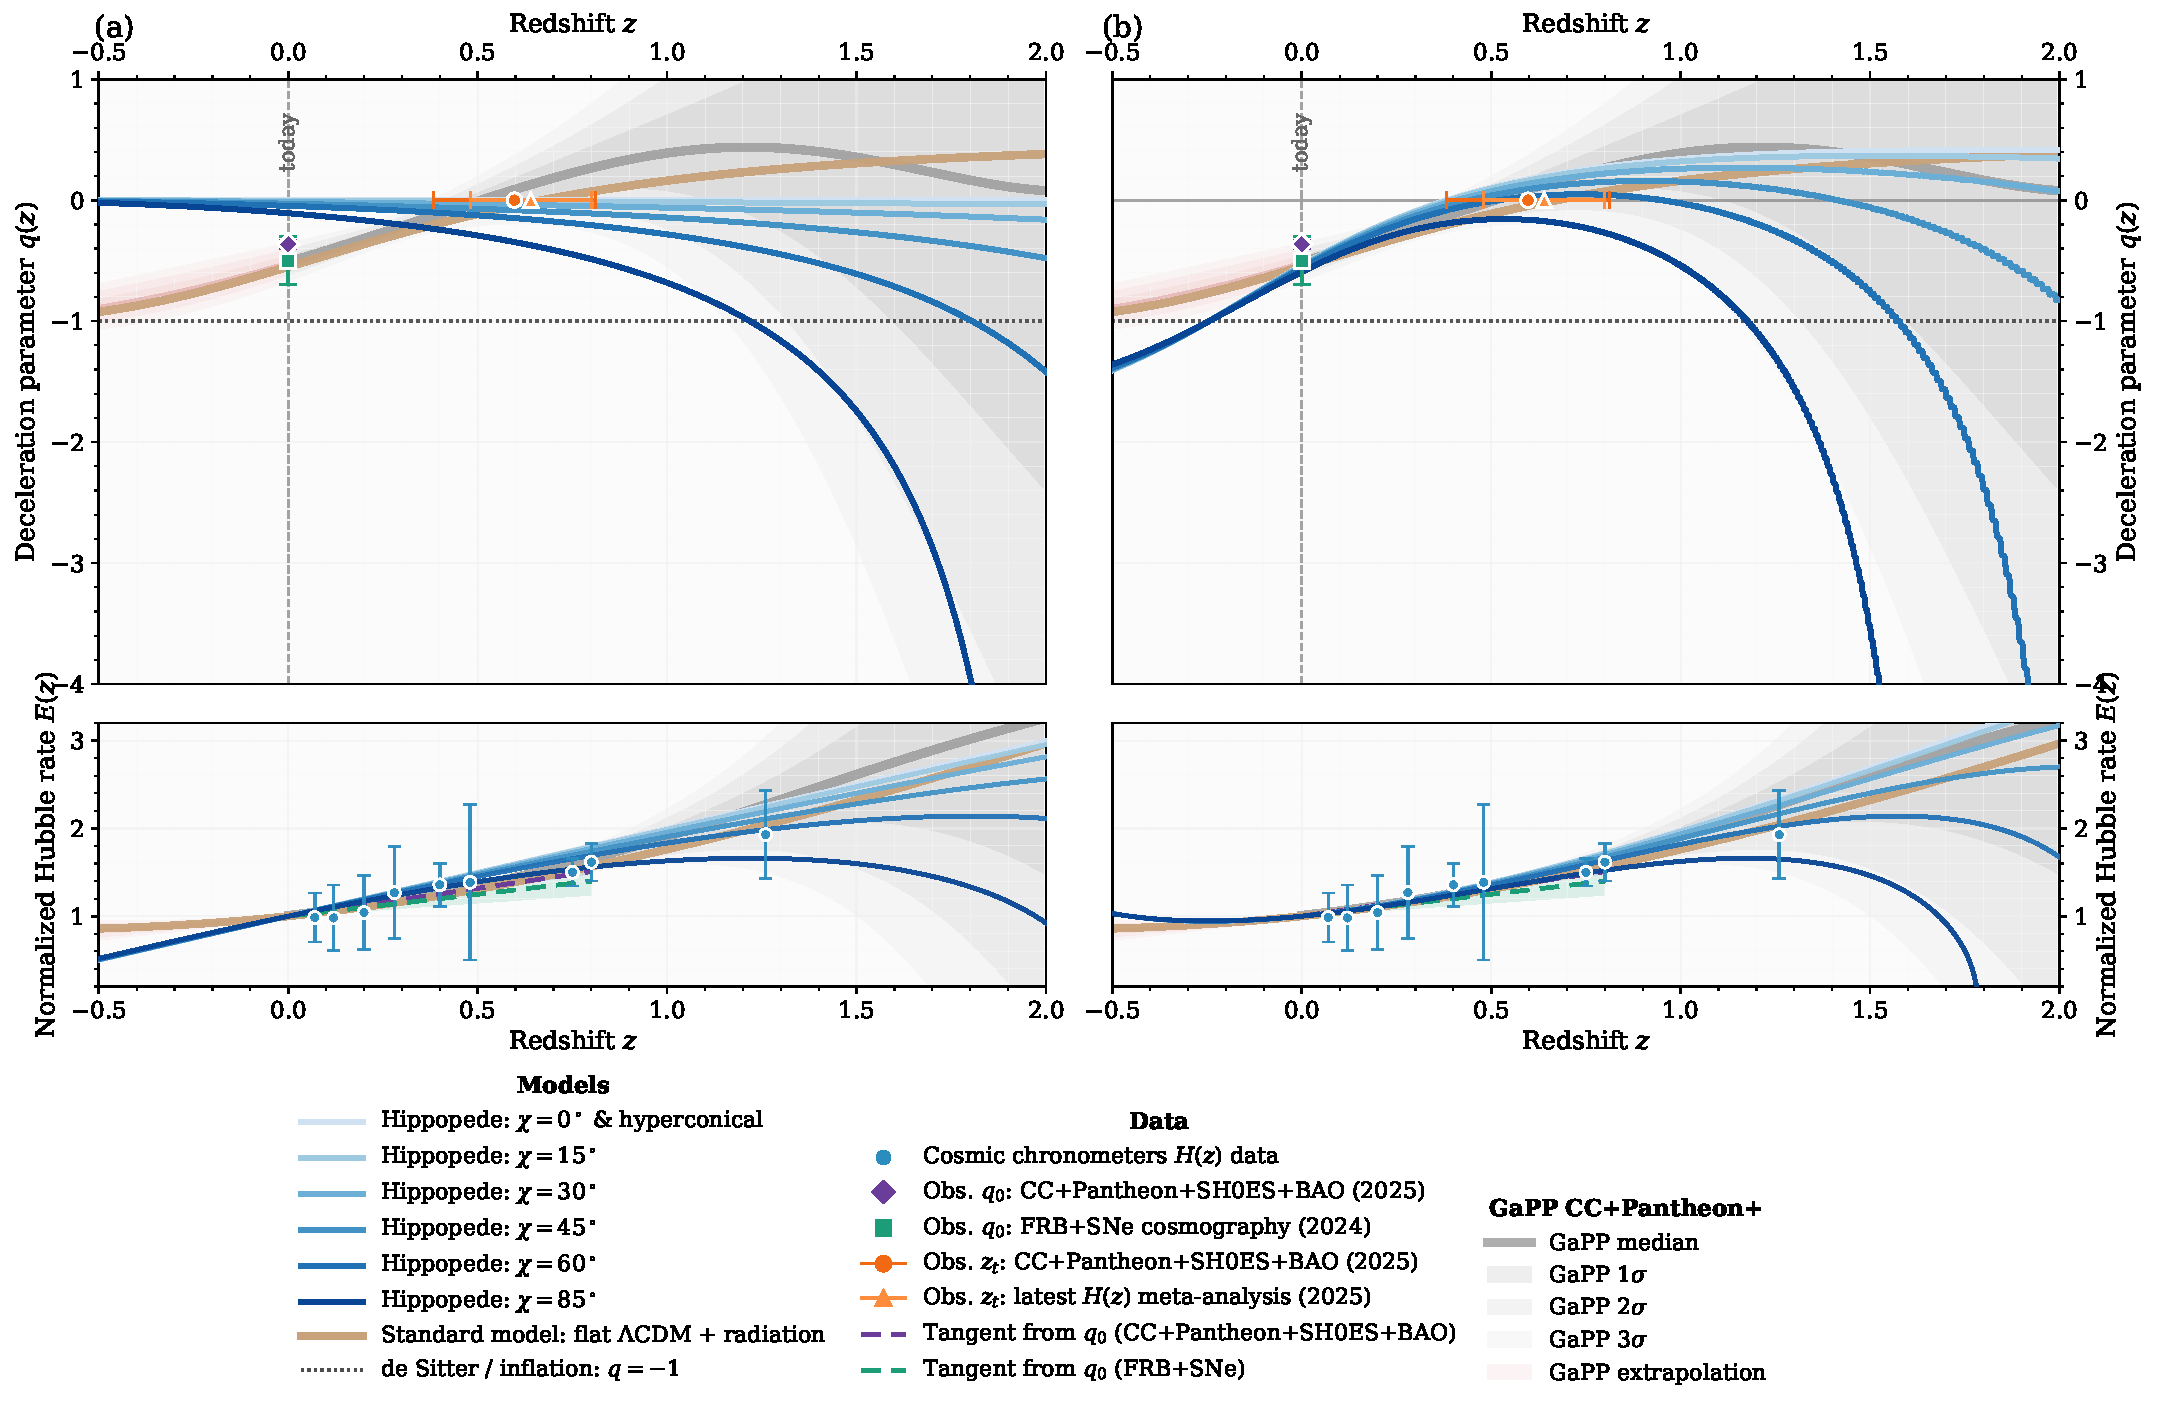
\includegraphics[width=\textwidth]{figures/hippopede_qz_centered_t0_3p0_double_panel_with_gapp}
\caption{
Comparison of the deceleration parameter $q(z)$ (top panels) and normalized expansion rate $E(z)=H(z)/H_0$ (bottom panels) for the centered-scale hippopede simulations (left block) and for the same centered histories after Monjo-type stereographic remapping (right block), both at fixed present time $t_0=3$. The colored curves correspond to the angular sectors $\chi=0^\circ,15^\circ,30^\circ,45^\circ,60^\circ,85^\circ$, while the thick light-brown curve shows the standard flat $\Lambda$CDM$+$radiation background. The upper panels include two present-day estimates of the deceleration parameter, $q_0=-0.364\pm0.032$ from CC+Pantheon+SH0ES+BAO and $q_0=-0.50\pm0.20$ from FRB+SNe cosmography, together with two transition-redshift determinations, $z_t=0.597\pm0.214$ and $z_t=0.64\pm0.16$ \cite{myrzakulov2025q0, gao2024frb, hu2025transition}. The lower panels include normalized cosmic-chronometer data and the GaPP reconstruction band obtained from CC+Pantheon$+$ data with the original Gaussian-process pipeline \cite{seikel2012gapp}. In the projected block the plotted value is $\alpha\simeq0.283$, following the preferred low-redshift implementation of \cite{monjo2018projected}; the Appendix explains why the same family also contains the asymptotic value $\alpha=1/2$ singled out by the radiation-like scaling requirement $H_{\mathrm{perc}}(T)\propto T^2$.}
\label{fig:qz_final}
\end{figure}

\subsection{Observational constraints on the projected model}

Applying the likelihood analysis described above to the DES-SN5YR supernova sample gives $\alpha_{\mathrm{eff}} = 0.323_{-0.012}^{+0.011}\;(1\sigma)$ with the result remaining stable across two independent \texttt{emcee} runs with different stretch-scale choices. Applying the same projected model to the DESI DR1 compressed BAO data gives $\alpha_{\mathrm{eff}} = 0.375_{-0.017}^{+0.016}\; (1\sigma)$, together with best-fit nuisance parameter $\beta = 28.85$ and $\chi^2_{\mathrm{best}}=12.39$ for 10 data points and 2 free parameters. For comparison, a flat $\Lambda$CDM fit with free $\Omega_m$ on the same BAO vector gives $\Omega_m = 0.289$ and $\chi^2_{\mathrm{best}}=11.72$, corresponding to $\Delta \mathrm{AIC}=0.68$. The two models are therefore statistically indistinguishable on the present DESI DR1 compressed BAO compilation.

\purple{Taken together, the supernova and BAO constraints probe distinct effective redshift ranges and remain consistent with a slow increase of the effective projection index relative to the low-redshift reference value $\alpha\simeq0.283$ discussed in \cite{monjo2018projected}.}

\begin{table}[h]
\centering
\color{purple}
\small
\caption{Summary of effective projected-hippopede constraints on $\alpha$.}
\label{tab:alpha_summary}
\begin{tabular}{lll}
\hline
Constraint & Redshift range & $\alpha_{\mathrm{eff}}$ \\
\hline
Low-$z$ projected reference \cite{monjo2018projected} & $z \rightarrow 0$ & 0.283 \\
DES-SN5YR \cite{abbott2024dark} & $0.025$--$1.3$ & $0.323_{-0.012}^{+0.011}$ \\
DESI DR1 BAO \cite{adame2025desi} & $0.295$--$1.491$ & $0.375_{-0.017}^{+0.016}$ \\
\hline
\end{tabular}
\end{table}



%The centered scale factor is defined on the $+u$ branch as $a_c^2=r^2+(u-t)^2$, and the corresponding directional redshift is given by $1+z_\chi=a_{c,\chi}(t_0)/a_{c,\chi}(t)$.

%The limit $\chi=0^\circ$ coincides with the hyperconical reference. The thick light-brown curve shows the standard flat $\Lambda$CDM background with radiation, while the dotted horizontal line marks the de Sitter reference $q=-1$.


At the same time, one should not overstate the analytical control of the projected model. The second-order analytic expansion used in the hyperconical literature is only a local approximation around $z=0$. In practice, the analytic approximation is useful only in a limited neighborhood of the present epoch; for the full displayed interval shown in the figure, the numerical prescription is the relevant one.

A second limitation concerns the interpretation of the projection parameter itself. The value $\alpha\simeq0.283$ gives the best low-redshift phenomenological agreement in the present implementation, but the projected family also contains the asymptotic value $\alpha=1/2$, which is selected by the high-redshift condition that the perceived thermal history satisfies $H_{\mathrm{perc}}(T)\propto T^2$. The two values need not be contradictory: the former can be understood as an effective late-time observational parameter, whereas the latter plays the role of a local/asymptotic physical limit in the sense discussed by Monjo and Campoamor-Stursberg \cite{monjo2020lagrangian, monjo2023hubble}.

\purple{At the purely geometric level, the same appendix also clarifies how the quartic hippopede can be read as a bilobulated deformation of the hyperconical picture, with axial branches that recover the hyperconical $3$-sphere limit and with a possible negative-curvature bilobulated extension described there as a separate geometric generalization rather than as part of the fitted late-time model.}

\blue{The same projected construction also suggests an effective observational isotropization toward high redshift. The anisotropy is clearly visible in the low-redshift dipole-like modulation, but the oblique sectors have a much shorter projected redshift reach than the nearly axial branch, so the observable window is expected to become progressively dominated by the preferred direction at sufficiently early apparent times. Since this point is directly relevant to the BBN-oriented interpretation, we discuss it in more detail in the Appendix.}

\subsubsection{\blue{Interpretation and limitations}}

Centered scale factor provides a cleaner phenomenological bridge between the quartic hypersurface and the asymptotic tangent-sphere picture than the origin-based scale factor. 

\blue{A separate numerical diagnostic indicates that the projected centered histories are indeed close to a dipole-like angular modulation over the low-redshift interval relevant to current background data. Fitting the projected $E(\chi,z)$ curves to the form $E_0(z)[1+D_1(z)\cos\chi]$ over the sectors $\chi=0^\circ$--$85^\circ$ yields $R^2\simeq0.98$--$0.99$ for $0.1\le z\le1$, with fitted amplitudes $D_1\simeq0.006$, $0.024$, $0.055$ and $0.231$ at $z=0.1$, $0.3$, $0.5$ and $1$, respectively. This does not yet constitute a fit to a sky dipole anomaly, because no mapping to an observed celestial direction has been imposed, but it does show that the anisotropy generated by the model is numerically very close to a true dipolar modulation over the late-time window where the observational comparison is performed.}

The present comparison remains exploratory. It is based on a selected set of chronometer and kinematic summary points, not on a full statistical fit, and it depends on a numerical pipeline that includes interpolation, differentiation, branch selection after the first minimum of $a_{c,\chi}(t)$, and, in the projected case, a specific implementation of the Monjo-type remapping. These limitations do not invalidate the qualitative comparison, but they do indicate that any stronger observational claim should be postponed to a dedicated fitting analysis.


\section{Discussion and conclusions}

The hippopede universe is not obtained from a constant-curvature hyperboloid but from a null quadratic relation in an auxiliary ambient (2,4)-spacetime as for an AdS${}_5$ manifold, and the quartic nature of the physical hypersurface arises because the embedding variables depend nonlinearly on the coordinates. In this sense the model should be viewed neither as a standard dS/AdS spacetime nor as a pure hyperconical cone, but rather as an intermediate toy geometry in which the ambient-space quadratic structure survives while the induced 4-dimensional hypersurface acquires a richer anisotropic dynamics.

To avoid a possible misunderstanding, one should emphasize that the toy universe is not identified with the full null hypersurface of the $(2,4)$ ambient space. The latter would be five-dimensional. What is physically relevant here is a four-dimensional submanifold satisfying both the null relation and the angular compatibility condition $u = \rho\cos\chi$, or equivalently the immersed image of the physical variables inside that null hypercone with $u$-axis constraint.

The cleanest way to compare the constructions is to separate three layers. First, the hippopede is recovered from a quartic constraint in Euclidean variables. Second, the toy universe lifts that quartic relation to a $t$-dependent hypersurface in $\mathbb{R}^{1,4}$ whose asymptotic radius is hyperconical-like. Third, after introducing auxiliary coordinates such as $p=(2t\cos\chi,\sin\chi, \vec{\rho}) \in \mathbb{R}^{2,4}$, the same quartic relation is rewritten by constraining the $u$-axis of the null quadratic condition $\|p\|_{\scriptscriptstyle{(2,4)}}^2=0$ in a $(2,4)$-signature ambient space, the same as for an AdS${}_5$ universe. The quartic character of our 4D hippopede universe is therefore not lost; it is encoded in the nonlinear way in which the physical coordinates enter the auxiliary null cone.

In this sense, the dS/AdS hyperboloids, their degenerate null-cone limits, and the hippopede null condition all belong to the same ambient-space family of quadratic loci, although they correspond to different geometric realizations. The relation among them is therefore one of shared embedding structure rather than dynamical equivalence. In fact, the same quartic relation defines a toy expanding geometry whose large-$t$ limit reproduces the linear law associated with hyperconical models, but whose subleading term produces an early-time regularization and a direction-dependent acceleration. The model is best understood as a controlled anisotropic toy universe: simple enough to admit closed analytic expressions, yet nontrivial enough to test how far one can deform exact hyperconical coasting while preserving its large-time behaviour.


%The geometric and cosmological lessons of the construction can be summarized in a compact way. Geometrically, the hippopede furnishes an explicit bridge between a classical quartic curve and the null quadratic constraints familiar from ambient-space relativity. Cosmologically, its four-dimensional extension shows that an asymptotically linear late expansion can coexist with a very different early-time acceleration pattern. 

\section*{\blue{Data Availability}}

\blue{The numerical scripts used to generate the figures are included in the project folder together with the local data files required for the final four-panel comparison figure. In particular, Fig.~\ref{fig:hippopede_growth_3d} is produced by \texttt{plot\_hippopede\_growth\_3d.py}, whereas Fig.~\ref{fig:qz_final} is produced by \texttt{plot\_hippopede\_qz\_double\_panel\_with\_gapp.py}. The supplementary diagnostic script \texttt{analyze\_hippopede\_dipole\_bbn.py} reproduces the late-time dipole-like fit and the constant-$\alpha$ BBN-oriented thermal checks reported in the main text and Appendix, while \texttt{analyze\_hippopede\_variable\_alpha.py} reproduces the running-$\alpha$ scans discussed in the Appendix. The dedicated thermal-history comparison against the standard radiation curve and the observationally inferred BBN corridor is generated by \texttt{plot\_hippopede\_projected\_thermal\_history\_bbn.py}. The bundled data directory contains the curated CC/BAO compilation, the local binned Pantheon$+$ input used by the GaPP reconstruction, and the local copy of the GaPP code needed to reproduce the figure.}

\bibliographystyle{unsrt}
\bibliography{main-hippopede}


\section*{Appendix}

\subsubsection*{Late-epoch linear expansion} 

The description of the hyppopede universe produces an anisotropic acceleration. If one now reads $t$ as a cosmic parameter for the origin-prescription approach and keeps the angular sector $\chi$ fixed, the directional scale factor of this toy model is
\begin{equation}
a_\chi(t):=\rho(t,\chi)=\sqrt{\sin^2\chi+4t^2\cos^2\chi}.
\end{equation}
In this origin-prescription focus, its directional Hubble, acceleration and deceleration functions are then
\begin{equation}
H_\chi(t)=\frac{\dot a_\chi}{a_\chi}=\frac{4t\cos^2\chi}{\sin^2\chi+4t^2\cos^2\chi},
\end{equation}
\begin{equation}
\ddot a_\chi(t)=\frac{4\cos^2\chi\,\sin^2\chi}{\left(\sin^2\chi+4t^2\cos^2\chi\right)^{3/2}},
\end{equation}
\begin{equation}
q_\chi(t):=-\frac{a_\chi\ddot a_\chi}{\dot a_\chi^2}=-\frac{\tan^2\chi}{4t^2}.
\end{equation}
Therefore the model is mildly accelerated for every oblique direction $0<|\chi|<\pi/2$, but the acceleration decays rapidly and
\begin{equation}
H_\chi(t)=\frac{1}{t}+O(t^{-3}),\qquad \ddot a_\chi(t)=\frac{\sin^2\chi}{2|{\cos\chi}|\,t^3}+O(t^{-5}),\qquad q_\chi(t)\to0^-.
\end{equation}
This is the precise sense in which the hippopede universe approaches linear expansion at late times: the asymptotic law is coasting, $a_\chi(t)\sim 2|{\cos\chi}|\,t$, even though the early epoch can display a nonzero positive acceleration. The limiting cases are also transparent: $\chi=0$ gives $a_0(t)=2t$ and hence exact linear expansion for all $t$, while $\chi=\pi/2$ gives $a_{\pi/2}(t)=1$, i.e. no expansion in the purely transverse direction. Numerically, for $\chi=\pi/4$ one finds $q_{\pi/4}(1)=-0.25$, $q_{\pi/4}(2)=-0.0625$, and $q_{\pi/4}(10)=-0.0025$, so the deviation from the linear regime dies off quickly.

\subsubsection*{Early-epoch accelerated universe}



The opposite limit is also informative. For any fixed oblique direction with $\sin\chi\neq0$,
\begin{equation}
a_\chi(0)=|\sin\chi|,\qquad \dot a_\chi(0)=0,\qquad \ddot a_\chi(0)=\frac{4\cos^2\chi}{|\sin\chi|}.
\end{equation}
Since $q_\chi(t)=-\tan^2\chi/(4t^2)$, the deceleration parameter is not merely large near $t=0$; it diverges to $-\infty$ for every fixed oblique direction with $\chi\neq0$. Numerically, for $\chi=\pi/6$ one finds $q_\chi(1)=-0.0833$, $q_\chi(0.5)=-0.333$, and $q_\chi(0.1)=-8.33$, while for $\chi=\pi/4$ the corresponding values are $-0.25$, $-1$, and $-25$. Thus the model becomes extremely accelerated at early times unless one approaches the privileged axis $\chi=0$. If one wishes to compare the toy model with observationally inferred $q(z)$, the next step would be to introduce an effective isotropized scale factor $a_{\mathrm{eff}}(t)$ and then use $1+z=a_{\mathrm{eff}}(t_0)/a_{\mathrm{eff}}(t)$ to map the directional dynamics into redshift space. A dedicated fit is therefore possible, but it requires an additional averaging prescription and should probably be presented separately as a numerical extension rather than as part of the conceptual derivation given here.
Hence the toy universe does not shrink to a point uniformly as $t\to0$: most angular sectors retain a finite initial radius and start with vanishing expansion rate but positive acceleration. The axis $\chi=0$ is singular in this limit, since $a_0(t)=2t$ collapses linearly to zero while the oblique sectors remain finite. This nonuniform behaviour is another sign that the model should be read as a biaxial toy geometry rather than as a realistic isotropic cosmology.


\subsubsection*{Bilobulated interpretation, axial hyperconical limit, and a possible $K=-1$ extension}

The large-$t$ geometry of the quartic model is best interpreted in two complementary ways. In the origin-based description one has
\begin{equation}
\rho(t,\chi)=\sqrt{\sin^2\chi+4t^2\cos^2\chi}
=2|{\cos\chi}|\,t+\frac{\sin^2\chi}{4|{\cos\chi}|\,t}+O(t^{-3}),
\end{equation}
so the leading term reproduces the dipolar law of the two tangent $3$-spheres discussed in the main text. Since the hyperconical universe of Monjo is foliated by spatial $3$-spheres of radius proportional to $t$, this is the precise sense in which each axial branch of the hippopede approaches a hyperconical branch at late times. Along the preferred directions $\chi\approx0$ and $\chi\approx\pi$, the quartic model therefore recovers the same linear coasting behaviour as the hyperconical construction, while the oblique sectors retain the anisotropic correction encoded in the subleading term.

The centered description clarifies the geometry of each individual lobe. On the $+u$ branch we defined
\begin{equation}
a_{c,\chi}(t):=\sqrt{r^2+(u-t)^2}
=\sqrt{\rho(t,\chi)^2+t^2-2t\,\rho(t,\chi)\cos\chi}.
\end{equation}
Using the same large-$t$ expansion for $\rho(t,\chi)$ one finds
\begin{equation}
a_{c,\chi}(t)^2
=t^2+\frac{\sin^2\chi}{2}+O(t^{-2}),
\qquad
a_{c,\chi}(t)
=t+\frac{\sin^2\chi}{4t}+O(t^{-3}).
\end{equation}
Thus, when each branch is viewed from the center of curvature of its own asymptotic tangent sphere, the lobe tends to a linearly expanding spatial $3$-sphere. This is again compatible with the hyperconical picture, because the constant-time spatial sections of the latter are themselves $3$-spheres. The difference is therefore mainly one of viewpoint: the origin-based picture emphasizes the dipolar two-branch structure, whereas the centered picture emphasizes the local recovery of a single hyperconical lobe.

This also shows why the bilobulated interpretation is close to, but not identical with, the quartic hippopede. The neck joining the two asymptotic lobes is certainly the most visible new geometric feature, but it is not the only one. Away from the strict large-$t$ limit the quartic relation leaves a residual angular deformation throughout the profile, and this is precisely what produces the anisotropic correction
\begin{equation}
\rho(t,\chi)-2|{\cos\chi}|\,t
=\frac{\sin^2\chi}{4|{\cos\chi}|\,t}+O(t^{-3}).
\end{equation}
In that sense, the hippopede should be viewed as a bilobulated hyperconical deformation: the neck expresses the global two-lobe topology, while the quartic angular term controls how the geometry departs from a pair of exact hyperconical branches at finite $t$.

The same intuition suggests a natural negative-curvature extension, although this goes beyond the exact quartic model studied in the main text. One may consider a compact hyperbolic $3$-manifold $N$ with totally geodesic boundary $\partial N\cong\Sigma_g$, where $\Sigma_g$ is a closed surface of genus $g\ge2$, and form the double
\begin{equation}
M_g=N\cup_{\phi}\bar N,
\end{equation}
with $\phi:\Sigma_g\to\Sigma_g$ an orientation-reversing boundary isometry. The resulting closed manifold carries a smooth metric of constant sectional curvature $K=-1$ and provides a mathematically natural bilobulated space with a geodesic neck. A cosmological line element of the form
\begin{equation}
ds^2=-dt^2+a(t)^2 h_{ij}dx^i dx^j,
\end{equation}
with $h_{ij}$ the hyperbolic metric on $M_g$, then defines a negatively curved FRW-type extension of the same bilobulated intuition.

However, this $K=-1$ construction should be interpreted carefully. The standard geodesic-polar expression
\begin{equation}
d\ell^2=d\rho^2+\sinh^2\rho\,d\Omega_2^2
\end{equation}
describes the simply connected space $H^3$ around a chosen point, not the full global geometry of a compact double $M_g$. Likewise, the quartic hippopede relation is not literally recovered as a global section of an arbitrary hyperbolic double. The connection is therefore structural rather than exact: the quartic model provides the explicit anisotropic toy geometry studied in this paper, whereas the doubled hyperbolic manifolds furnish a natural family of bilobulated negative-curvature analogues in which the neck is global and the asymptotic hyperconical intuition is replaced by hyperbolic ends or local axial neighbourhoods. The present work establishes the former rigorously and leaves the latter as a plausible geometric extension for future study.


\subsubsection*{Projected thermal asymptotics and the BBN-motivated limit $\alpha=1/2$}

To discuss primordial nucleosynthesis in the projected picture, one must distinguish between the intrinsic geometric time and the perceived thermal history of the projected radiation sector. The latter is the relevant quantity for BBN. Assuming the minimal adiabatic identification $T_{\mathrm{perc}}\propto 1+z$ (up to the usual slowly varying entropy factor $g_{*S}$), the high-redshift behaviour of the projected Hubble function follows directly from the asymptotics of the Monjo-type projection.

For $k=1$ one has $x_{\max}=\sqrt{3}/2$ and $b(x)=\sqrt{1-x^2}$, with $b(x_{\max})=1/2$. Writing $x=x_{\max}-\delta$ with $\delta\downarrow0$, one finds
\begin{equation}
2b-1\;=\;2\sqrt{1-x^2}-1\;=\;-2\sqrt{3}\,\delta+O(\delta^2),
\end{equation}
while
\begin{equation}
\sqrt{1-(1-b)^2}=\sqrt{2b-b^2}=\frac{\sqrt{3}}{2}+O(\delta).
\end{equation}
Therefore the line-of-sight integrand behaves as
\begin{equation}
\frac{\sqrt{1-(1-b)^2}}{b[2(b-1)+1]}
\;=\; -\frac{1}{2\delta}+O(1),
\end{equation}
so that
\begin{equation}
\xi_1(x)= -\frac12\ln\delta + O(1).
\end{equation}
Since $\xi_1(x)=\ln(1+z)$, this implies the boundary relation
\begin{equation}
\delta=x_{\max}-x(z)\propto (1+z)^{-2}.
\end{equation}

Now define $\eta:=\gamma_0-\gamma(x)$. Because $\gamma'(x)=1/\sqrt{1-x^2}$ is finite at $x=x_{\max}$, one has $\eta\propto\delta$. Near the boundary, the Monjo-type projection
\begin{equation}
f_{\hat r}^{\alpha}(x)=2\arctan\!\left[\frac{\gamma(x)/2}{(1-\gamma(x)/\gamma_U)^\alpha}\right]
\end{equation}
obeys
\begin{equation}
\frac{df_{\hat r}^{\alpha}}{dx}\propto \eta^{\alpha-1}\propto \delta^{\alpha-1}.
\end{equation}
Combining this with $dx/dz\propto (1+z)^{-3}$ gives
\begin{equation}
\frac{d\hat r}{dz}\propto (1+z)^{-(1+2\alpha)},
\qquad
\hat H(z)=\left(\frac{d\hat r}{dz}\right)^{-1}\propto (1+z)^{1+2\alpha}.
\end{equation}
Hence the projected family satisfies the asymptotic law
\begin{equation}
E_{\mathrm{hyp}}^{\mathrm{proj}}(z)\propto (1+z)^n,
\qquad n=1+2\alpha.
\end{equation}
Under the perceived thermal identification $T_{\mathrm{perc}}\propto 1+z$, this becomes
\begin{equation}
H_{\mathrm{perc}}(T)\propto T^{1+2\alpha}.
\end{equation}
The radiation-dominated standard law $H(T)\propto T^2$ is therefore recovered precisely when
\begin{equation}
\alpha=\frac12.
\end{equation}

\blue{The asymptotic exponent, however, is only part of the BBN requirement. A direct numerical calibration of the same projected prescription, performed with the extended lookup implemented in \texttt{analyze\_hippopede\_dipole\_bbn.py}, gives $n_{\mathrm{eff}}=1.999999$ over the interval $10^3\lesssim z\lesssim10^6$, as expected for $\alpha=1/2$, but the corresponding physical normalization obtained from $H_{\mathrm{perc}}(T)=H_0E_{\mathrm{hyp}}^{\mathrm{proj}}(T/T_0-1)$ is still too large by an approximately constant factor $H_{\mathrm{perc}}/H_{\mathrm{rad}}\simeq10.2$ in the representative BBN temperature range $T\simeq0.07$--$1\,\mathrm{MeV}$ when compared with the standard radiation-era law. Thus the constant-$\alpha$ branch with $\alpha=1/2$ reproduces the correct $T^2$ scaling but not yet the standard normalization.}

\blue{This observation motivates a second, more flexible numerical test within the same projected family: instead of identifying a single constant projection index, one may allow a smooth perceived-history interpolation}
\begin{equation}
\blue{
\alpha(z)=\alpha_{\mathrm{low}}+\frac{\alpha_{\mathrm{high}}-\alpha_{\mathrm{low}}}{2}
\left[
1+\tanh\!\left(
\frac{\ln(1+z)-\ln(1+z_c)}{2}
\right)
\right],
}
\end{equation}
\blue{with $\alpha_{\mathrm{low}}=0.283$ fixed by the successful low-redshift phenomenology of Fig.~\ref{fig:qz_final}, and $\alpha_{\mathrm{high}}=1/2$ fixed by the radiation-like asymptotic requirement. Exploratory scans with the supplementary script \texttt{analyze\_hippopede\_variable\_alpha.py}, checked directly against the literal projected-map relation $H_{\mathrm{perc}}(T)=H_0E_{\mathrm{hyp}}^{\mathrm{proj}}(T/T_0-1)$, show that the most promising BBN-like window is obtained for an earlier and narrower transition, approximately around}
\begin{equation}
\blue{
z_c\sim 1.6\times10^4
}
\end{equation}
\blue{This choice preserves the low-redshift sector almost unchanged, since $\alpha(1)\simeq0.28302$ and $\alpha(2)\simeq0.28303$, while driving the projected thermal history very close to the standard radiation-era normalization across the BBN window. In the updated diagnostic we compare it directly with the observationally inferred BBN corridor obtained from the 2024 primordial-abundance fit $\Delta N_{\mathrm{eff}}=-0.10\pm0.21$ of \cite{schoneberg2024bbn}. A representative near-optimal case is}
\begin{equation}
\blue{
z_c=1.616\times10^4
}
\end{equation}
\blue{for which the geometric-mean normalization with respect to the standard radiation curve over the interval $T\simeq0.07$--$1\,\mathrm{MeV}$ is}
\begin{equation}
\blue{
\left\langle \frac{H_{\mathrm{perc}}}{H_{\mathrm{rad}}}\right\rangle_{\mathrm{geom}}
\simeq 0.9915,
}
\end{equation}
\blue{with pointwise values}
\begin{equation}
\blue{
\frac{H_{\mathrm{perc}}}{H_{\mathrm{rad}}}\approx
0.991,\ 0.992,\ 0.993,\ 0.991,\ 0.991
}
\end{equation}
\blue{at $T=0.07,\ 0.10,\ 0.20,\ 0.50,\ 1.0\,\mathrm{MeV}$, respectively. Relative to the BBN-inferred central history of \cite{schoneberg2024bbn}, the corresponding residuals are only $-1.2\times10^{-3},\ 4.0\times10^{-4},\ 1.0\times10^{-3},\ -1.2\times10^{-3},\ -6.3\times10^{-4}$ over the same five temperatures. In the plotted diagnostic these values are read from the same literal projected-map evaluation after the mild log-space smoothing mentioned above, which removes small non-physical spikes produced by numerical differentiation of the dense lookup table without changing the BBN-window normalization in any material way. In other words, the same projected family admits a smooth perceived thermal history for which the whole BBN window is brought extremely close not only to the standard radiation background, but also to the currently inferred observational BBN corridor, rather than remaining strongly suppressed in the low-redshift constant-$\alpha$ branch or enhanced by more than one order of magnitude in the pure $\alpha=1/2$ branch.}

\blue{This does not yet amount to a full light-element calculation, and we therefore do not claim in this paper that the primordial abundances are already reproduced in detail. Nevertheless, the numerical result is strong enough to support a more focused statement: within the projected-hyperconical interpretation, the apparent thermal history can be made quantitatively compatible with both the normalization and the asymptotic $T^2$ scaling expected for a BBN-like radiation era, provided one allows a smooth transition from the low-redshift phenomenological value $\alpha\simeq0.283$ to the asymptotic physical value $\alpha=1/2$. A complete BBN claim would then require the next layer of analysis, namely a consistent treatment of $g_{*S}(T)$, the weak-interaction freeze-out, and the light-element reaction network.}

\blue{The same numerical exploration clarifies how the inherited anisotropy enters the projected early-time discussion. If one tries to construct a genuinely sector-dependent quantity}
\begin{equation}
\blue{
R_\chi(T):=\frac{H_{\chi,\mathrm{perc}}(T)}{H_{\mathrm{rad}}(T)},
}
\end{equation}
\blue{using the projected centered histories themselves, one finds that each fixed angle $\chi$ has only a finite internal redshift support. For the centered branches adopted in this work, the maximum unprojected redshifts are approximately}
\begin{equation}
\blue{
z^*_{\max}\simeq 3.0\times10^4,\ 12.36,\ 5.87,\ 3.78,\ 2.80,\ 2.13
}
\end{equation}
\blue{for $\chi=0^\circ$, $15^\circ$, $30^\circ$, $45^\circ$, $60^\circ$ and $85^\circ$, respectively. When these endpoints are translated back through the common projected-hyperconical map with $\alpha=1/2$, they correspond only to}
\begin{equation}
\blue{
z_{\mathrm{obs},\max}\simeq 422,\ 7.64,\ 5.01,\ 3.87,\ 3.23,\ 2.74,
}
\end{equation}
\blue{or, equivalently, to perceived temperatures of order}
\begin{equation}
\blue{
T_{\max}\simeq 9.9\times10^{-8},\ 2.0\times10^{-9},\ 1.4\times10^{-9},\ 1.1\times10^{-9},\ 1.0\times10^{-9},\ 8.8\times10^{-10}\ \mathrm{MeV}.
}
\end{equation}
\blue{These scales lie far below the standard BBN window $T\sim0.07$--$1\,\mathrm{MeV}$. Therefore the present centered branch does not yet provide a full anisotropic BBN calculation sector by sector: the oblique projected histories simply terminate long before one reaches the redshifts relevant to primordial nucleosynthesis.}

\blue{This is nevertheless physically informative. It means that the stereographic remapping does not erase the underlying anisotropy, but it does strongly filter its observational visibility. The oblique sectors dominate the low-redshift phenomenology and are responsible for the dipole-like modulation discussed in the main text, whereas at sufficiently high apparent redshift the observer progressively loses access to those sectors and is left mainly with the nearly axial branch. In that sense the projected model suggests an effective observational isotropization toward high redshift: the background remains intrinsically anisotropic, yet the observable radiation history becomes increasingly dominated by the preferred direction. The running-$\alpha$ BBN-like result obtained above should therefore be interpreted as an effective perceived thermal history of the projected radiation sector, not as a complete primordial-nucleosynthesis solution on the anisotropic centered background itself.}

\end{document}


